\documentclass[a4paper,11pt,twoside]{article}

\usepackage{my-thesis-template}


%----------------------------------------------------------------------------------------
%	METADATA
%----------------------------------------------------------------------------------------
\newcommand{\thesistitle}{Robotic surgical tool manipulator - Recognition, control and manipulation of laparoscopic tools}
\newcommand{\division}{Division}
\newcommand{\me}{Karadimos Alexios of Loukas}
\newcommand{\nomme}{Karadimos Alexios of Loukas}
\newcommand{\studnum}{1046820}
\newcommand{\monthyear}{Month 2021}
\newcommand{\supname}{Evangelos Dermatas}
\newcommand{\suptitle}{Associate Professor Dr.}
\newcommand{\cosupname}{Anthony Tzes}
\newcommand{\cosuptitle}{Professor Dr.}
\newcommand{\headofdivision}{Kazakos Demosthenes}
\newcommand{\headofdivisiontitle}{Assistant Professor Dr.}
\newcommand{\keywords}{surgery, robotics, control, laparoscopy}
\title{\thesistitle}
\author{Karadimos Alexios}
\date{2020}

% PDF metadata
\hypersetup
{
    pdfauthor={Alexios Karadimos},
    pdftitle={thesis},
    pdfsubject={\thesistitle},
    pdfkeywords={\keywords},
    pdfproducer={PdfLaTex},
    pdfcreator={Alexios Karadimos}
}


\begin{document}

\selectlanguage{greek}
\selectlanguage{english}


%----------------------------------------------------------------------------------------
%	FRONT PAGE & CERTIFICATION
%----------------------------------------------------------------------------------------
\begin{titlepage}
\begin{center}
% Upper part of the page
\textsc{\textbf{\large UNIVERSITY OF PATRAS - SCHOOL OF ENGINEERING}\\
\large DEPARTMENT OF ELECTRICAL AND COMPUTER ENGINEERING}\\


\includegraphics[width= 0.5\textwidth]{up_2017_logo_gr.png}\\  

\textsc{Division: \large Systems and Automatic Control}\\[1cm]

\textsc{\textbf{\LARGE{Thesis}}}\\ [0.5cm]
of the student of the Department of Electrical and Computer Engineering of the School of Engineering of the University of Patras\\[0.5cm]

\textsc{\Large \me }\\[0.5cm]
\textsc{\large Student Number: 1046820}\\[1cm]

\underline{\large Subject}\\
\HRule \\[0.4cm]
{\huge \bfseries \thesistitle }\\[0.4cm] % Title of your document
\HRule \\[1.5cm]

\underline{\large Supervisor}\\[0.5cm]
\large \suptitle \, \supname \\[1cm]
\textbf{Thesis Number:}
%\large 1046820/2020
\vfill
% Bottom of the page
\large{Patras, 2020}
\end{center}
\end{titlepage}

% \begin{titlepage}

% %----------------------------------------------------------------------------------------
% %	HEADING SECTIONS
% %----------------------------------------------------------------------------------------

% \Large UNIVERSITY OF PATRAS - SCHOOL OF ENGINEERING\\[0.5cm] % Name of your university/college
% \textsc{\Large DEPARTMENT OF ELECTRICAL AND COMPUTER ENGINEERING}\\[0.5cm] % Major heading such as course name
% \textsc{\large \textlatin{ECE}ΔΚ803}\\[0.5cm] % Minor heading such as course title

% %----------------------------------------------------------------------------------------
% %	TITLE SECTION
% %----------------------------------------------------------------------------------------


% %----------------------------------------------------------------------------------------
% %	AUTHOR SECTION
% %----------------------------------------------------------------------------------------


% % If you don't want a supervisor, uncomment the two lines below and remove the section above
% %\Large \emph{Author:}\\
% \emph{Αλέξιος Καραδήμος}\\ % Your name
% Τμήμα Ηλεκτρολόγων Μηχανικών \& Τεχνολογίας Υπολογιστών\\[2cm]

% %----------------------------------------------------------------------------------------
% %	DATE SECTION
% %----------------------------------------------------------------------------------------

% {\large 2020}\\[1cm] % Date, change the \today to a set date if you want to be precise

% %----------------------------------------------------------------------------------------
% %	LOGO SECTION
% %----------------------------------------------------------------------------------------

% \begin{center}
% 
\includegraphics[width=5cm]{images/up_2017_logo_gr.png}\\[1cm] % Include a department/university logo - this will require the graphicx package
% \end{center}

% %----------------------------------------------------------------------------------------

% \vfill % Fill the rest of the page with whitespace

% \end{titlepage}

\pagestyle{empty}
\begin{center}
{\LARGE \textbf{ΠΙΣΤΟΠΟΙΗΣΗ}\\[1cm]}
\large Πιστοποιείται ότι η διπλωματική εργασία με θέμα\\[1cm]
\textbf{\large \thesistitle }\\[1cm]
του φοιτητή του Τμήματος Ηλεκτρολόγων Μηχανικών και Τεχνολογίας Υπολογιστών\\[1.5cm]
\me \\[0.5cm]
(Α.Μ.: \studnum )\\[1.5cm]
παρουσιάστηκε δημόσια και εξετάστηκε στο τμήμα  Ηλεκτρολόγων Μηχανικών και Τεχνολογίας Υπολογιστών στις\\[1cm]
\Large{\_\_/\_\_/\_\_\_}\\[1.5cm]
\end{center}
\begin{minipage}{0.5\textwidth}
\begin{flushleft} \large
Ο Επιβλέπων\\[4cm]
\supname \\
\emph{\suptitle}
\end{flushleft}
\end{minipage}
\begin{minipage}{0.5\textwidth}
\begin{flushright} \large
Ο Διευθυντής του Τομέα\\[4cm]
\headofdivision\\
\emph{\headofdivisiontitle}
\end{flushright}
\end{minipage}

\newpage{\pagestyle{empty}\cleardoublepage}
\newpage
\pagestyle{empty}
\begin{center}
{\LARGE \textbf{CERTIFICATION}\\[1cm]}
\large It is certified that the Thesis with Subject\\[1cm]
\textbf{\large \thesistitle }\\[1cm]
of the student of the Department of Electrical and Computer Engineering\\[1.5cm]
\me \\[0.5cm]
(R.N.: \studnum )\\[1.5cm]
Was presented publicly and defended at the Department of Electrical and Computer Engineering at\\[1cm]
\Large{\_\_/\_\_/\_\_\_}\\[1.5cm]
\end{center}
\begin{minipage}{0.5\textwidth}
\begin{flushleft} \large
The supervisor\\[4cm]
\supname \\
\emph{\suptitle}
\end{flushleft}
\end{minipage}
\begin{minipage}{0.5\textwidth}
\begin{flushright} \large
The Director of the Division\\[4cm]
\headofdivision\\
\emph{\headofdivisiontitle}
\end{flushright}
\end{minipage}

\pagestyle{empty}
\begin{center}

{\large \textbf{Thesis details}\\[1cm]}

\textbf{\large \thesistitle }\\[1cm]

\pagestyle{empty}
{\textbf{Abstract}\\[1cm]}

This thesis studies all the stages involved in the perception, control and manipulation of robotic laparoscopic tools with emphasis given to the pivot trajectories and the RCM constrained motion planning. The forward and inverse kinematics of the 7 DoF KUKA iiwa14 industrial robot arm was studied  followed by kinematics of the attached Barrett hand gripper for grasping purposes. Minimal Invasive Surgery (MIS) necessitates the study of Remote Center-of-Motion (RCM)  constraint for the pivot motions, the elbow-up constraint to avoid collisions as well as the workspace constraints and singularities. The transformation of the surgical task space into the robot’s taskspace and the joint space is subsequently analyzed along with the robot's manipulability. Emphasis was given in calculating various geometric paths for the robot to follow inside the surgical task. The equations for circular, circular arc, line segment, helical, cubic spline, b-spline, higher-order polynomial and trapezoid and s-curve velocity profile trajectories are studied in detail in order to generate pivot motions with a wide variety. Simulations were conducted using the ROS framework and libraries like Gazebo, RViz and MoveIt using the RRTConnect path planning algorithm. The simulations were evaluated with measurements of time, position accuracy and RCM distance deviation. This thesis also briefly 
studies a simple recognition of a laparoscopic tool and the estimation of its position and orientation using computer vision as well as the calculation of three points on the surgical tool where the gripper’s fingers will be 
placed in order to grasp the object with a satisfactory force closure. Finally this thesis studies some control system schemes like for example the RCM tracking and pivot motion control.

\newpage{\pagestyle{empty}\cleardoublepage}

\newpage
\pagestyle{empty}
{\textbf{Περίληψη}\\[1cm]}

Η παρούσα διπλωματική εξετάζει όλα τα στάδια που εμπλέκονται στην αναγνώριση, τον έλεγχο και τον χειρισμό των λαπαροσκοπικών εργαλείων με μια ολιστική προσέγγιση αλλά με μεγαλύτερη έμφαση να δίνεται στις τροχιές περιστροφής 
γύρω από σημείο και στον προγραμματισμό περιορισμένης κίνησης RCM. Το πρώτο βήμα ήταν να μελετηθεί το ευθύ και αντίστροφο κινηματικό πρόβλημα του βιομηχανικού ρομποτικού βραχίονα KUKA iiwa14 (με την τεχνική αποσύνδεσης θέσης-
προσανατολισμού για ρομπότ 6 βαθμών ελευθερίας, αφήνοντας τον επιπλέον βαθμό ελευθερίας να καθοριστεί από άλλους περιορισμούς) καθώς και η κινηματική της αρπάγης Barrett ώστε να υπολογιστούν λαβές του χειρουργικού εργαλείου. 
Δεδομένου ότι η ρομποτική MIS επιβάλλει πολλούς περιορισμούς, το επόμενο βήμα ήταν να μελετηθεί ο περιορισμός RCM για τις κινήσεις περιστροφής (pivot), o περιορισμός στον οποίο ο αγκώνας του ρομπότ πρέπει να είναι προς τα πάνω 
για την αποφυγή συγκρούσεων καθώς και οι περιορισμοί και τα σημεία ενικότητας του χώρου εργασίας. Κατά το σχεδιασμό εφαρμογών ρομπότ είναι σημαντικό να μελετηθεί ο χώρος εργασίας του ρομπότ και για το λόγο αυτό, αυτή στη 
διπλωματική αυτή μελετάται επιπλέον ο χώρος χειρουργικών εργασιών και πώς αυτός μετατρέπεται στον χώρο εργασιών του ρομπότ και στον χώρο αρθρώσεών του. Μελετήθηκε επίσης ο δείκτης επιδεξιότητας του ρομπότ και η κατάλληλη 
διάταξη του ρομπότ σε σχεση με το περιβάλλον του έτσι ώστε όλες οι τροχιές να είναι καλά προσβάσιμες και να μπορουν να εκτελεστούν με ευκολία. Δόθηκε μεγάλη έμφαση στον υπολογισμό διαφόρων γεωμετρικών μονοπατιών που έπρεπε να 
ακολουθήσει το ρομπότ μέσα στο χώρο χειρουργικής εργασίας. Οι εξισώσεις για τροχιές κύκλου, κυκλικού τόξου, ευθύγραμμου τμήματος, έλικα, κυβικού spline, b-spline, πολυωνύμων υψηλότερης τάξης και τροχιές με προφίλ ταχύτητας 
τραπεζοειδές και καμπύλης-s, μελετώνται λεπτομερώς, προκειμένου να δημιουργηθούν χειρουργικές ρομποτικές κινήσεις με μεγάλη ποικιλία. Όλα τα πειράματα υλοποιήθηκαν χρησιμοποιώντας το περιβάλλον ROS και δημοφιλή εργαλεία και 
βιβλιοθήκες όπως τα Gazebo, RViz και MoveIt χρησιμοποιώντας τον αλγόριθμο σχεδιασμού διαδρομής RRTConnect. Τα πειράματα αξιολογήθηκαν με μετρήσεις χρόνου, ακρίβειας θέσης και απόκλισης απόστασης RCM. Στη διπλωματική αυτή 
μελετάται επίσης εν συντομία η απλή αναγνώριση ενός λαπαροσκοπικού εργαλείου και η εκτίμηση της θέσης και του προσανατολισμού του με χρήση υπολογιστικής όρασης καθώς και ο υπολογισμός 3 σημείων πάνω στο χειρουργικό εργαλείο 
όπου θα τοποθετηθούν τα δάχτυλα της αρπάγης για να πιάσει το αντικείμενο με μία ικανοποιητική λαβή. Τέλος, σε αυτή τη διπλωματική μελετώνται ορισμένα συστήματα ελέγχου όπως για παράδειγμα ενός συστήματος για την παρακολούθηση 
RCM και τον έλεγχο κίνησης περιστροφής.


\pagestyle{empty}
{\textbf{Αcknowledgements}\\[1cm]}

The subject of this thesis is a subject that I have been passionate about for many years and from the beginning of my university studies. For this reason
I would like to thank my supervisors, Evangelos Dermatas and Anthony Tzes, for their guidance and for giving me the opportunity to dive deep into this fascinating subject. I would also like to thank Nikolaos Evangeliou (PostDoctoral Associate at NYU Abu Dhabi) for giving me feedback on this thesis. Last but not least, I would like to thank my friends and family for their huge support and for pushing me during the pandemic to conquer my academic goals.




%----------------------------------------------------------------------------------------
%	TABLE OF CONTENTS
%----------------------------------------------------------------------------------------

\pagestyle{fancy}

\clearpage
\tableofcontents
\renewcommand*\contentsname{Table of Contents}

%----------------------------------------------------------------------------------------
%	MAIN SECTIONS
%----------------------------------------------------------------------------------------

\newpage
\section{Introduction}

\subsection{Surgery Robotics}

Surgery Robotics is a field of Surgery where the surgeon operaties on the patient via a computer, specialised equipment and robotic arms, 
to which the surgical tools needed for the operation are attached. According to surgical bibliography, robotics and laparoscopic procedures are used 
in general surgery, cardiothoracic surgeries, colon surgeries, gynecology, neurosurgery and orthopedics. \\

Robotic mechanisms were first introduced in Medicine, in 1987 with the first laparoscopic surgery of a cholecystectomy. Since then numerous laparoscopic 
operations have been performed and there has been a lot of improvements and innovations in this field. Such surgical operations are characterised as 
\textbf{minimally invasive}, because the surgical incisions made at the patient are very small and thus the probability of infection of the patient during 
or after the operation are very small, the hospitalization time is reduced (which means mean better and more efficient use of hospital resources) and the overall 
recovery of the patient is significantly faster and less painful. \\

However, traditional laparoscopic mechanisms have some downsides as well. First of all, the surgeon should operate in a mirrored-way, meaning that they should 
move at the opposite direction from what they saw at the screen (this effect is also known as the \textbf{fulcrum effect}), in order to reach the desired point of operation. Earlier laparoscopic tools had less 
degrees of freedom, which means less flexibility in motion control. Moreover these systems provided limited touch sensibility and feedback to the doctor they 
were very susceptible to the surgeon's micro movements and tremble. \\

The first application of robotics in Surgery appears in 1985, when Kwoh et al. \cite{Shao1985ANC} used a \textbf{PUMA 560}, a standard industrial robotic arm, to perform a neurosurgical biopsy, 
where the biopsy needle was inserted in the brain and guided with the help of Computed Tomography. This successful application was followed by the \textbf{PROBOT} surgical robot \cite{Probot1992}, 
which was developed at the Imperial College and used in a prostatectomy operation. Another example of an early surgery robot was the \textbf{ROBODOC} system \cite{Robodoc} developed by Integrated Surgical Supplies 
in Sacramento California, which was the first to be used in orthopedics for a hip replacement surgery and was also the first to be approved by the FDA (Food \& Drug Administration, organization responsible 
for medical devices, drugs etc.).

\begin{center}
\begin{figure}[H]
\centering
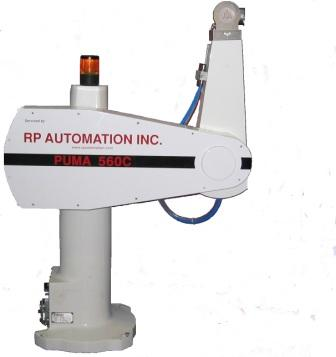
\includegraphics{images/Puma560.jpg}\\
\caption{The PUMA 560 robotic arm, which was the first to be used in surgery robotics in 1985}
\end{figure}
\end{center}

Some other important surgery robots are listed below:
\begin{itemize}
\item \textbf{AESOP\textsuperscript \textregistered Endoscope Positioner}
\item \textbf{HERMES\textsuperscript \textregistered Control Center}
\item \textbf{daVinci Surgical System\textsuperscript \textregistered}
\item \textbf{SOCRATES Robotic Telecollaboration System}
\item \textbf{Raven-II} \cite{Raven2}: An open platform for collaborative research on surgical robotics.
\end{itemize}

\begin{center}
\begin{figure}[H]
\centering
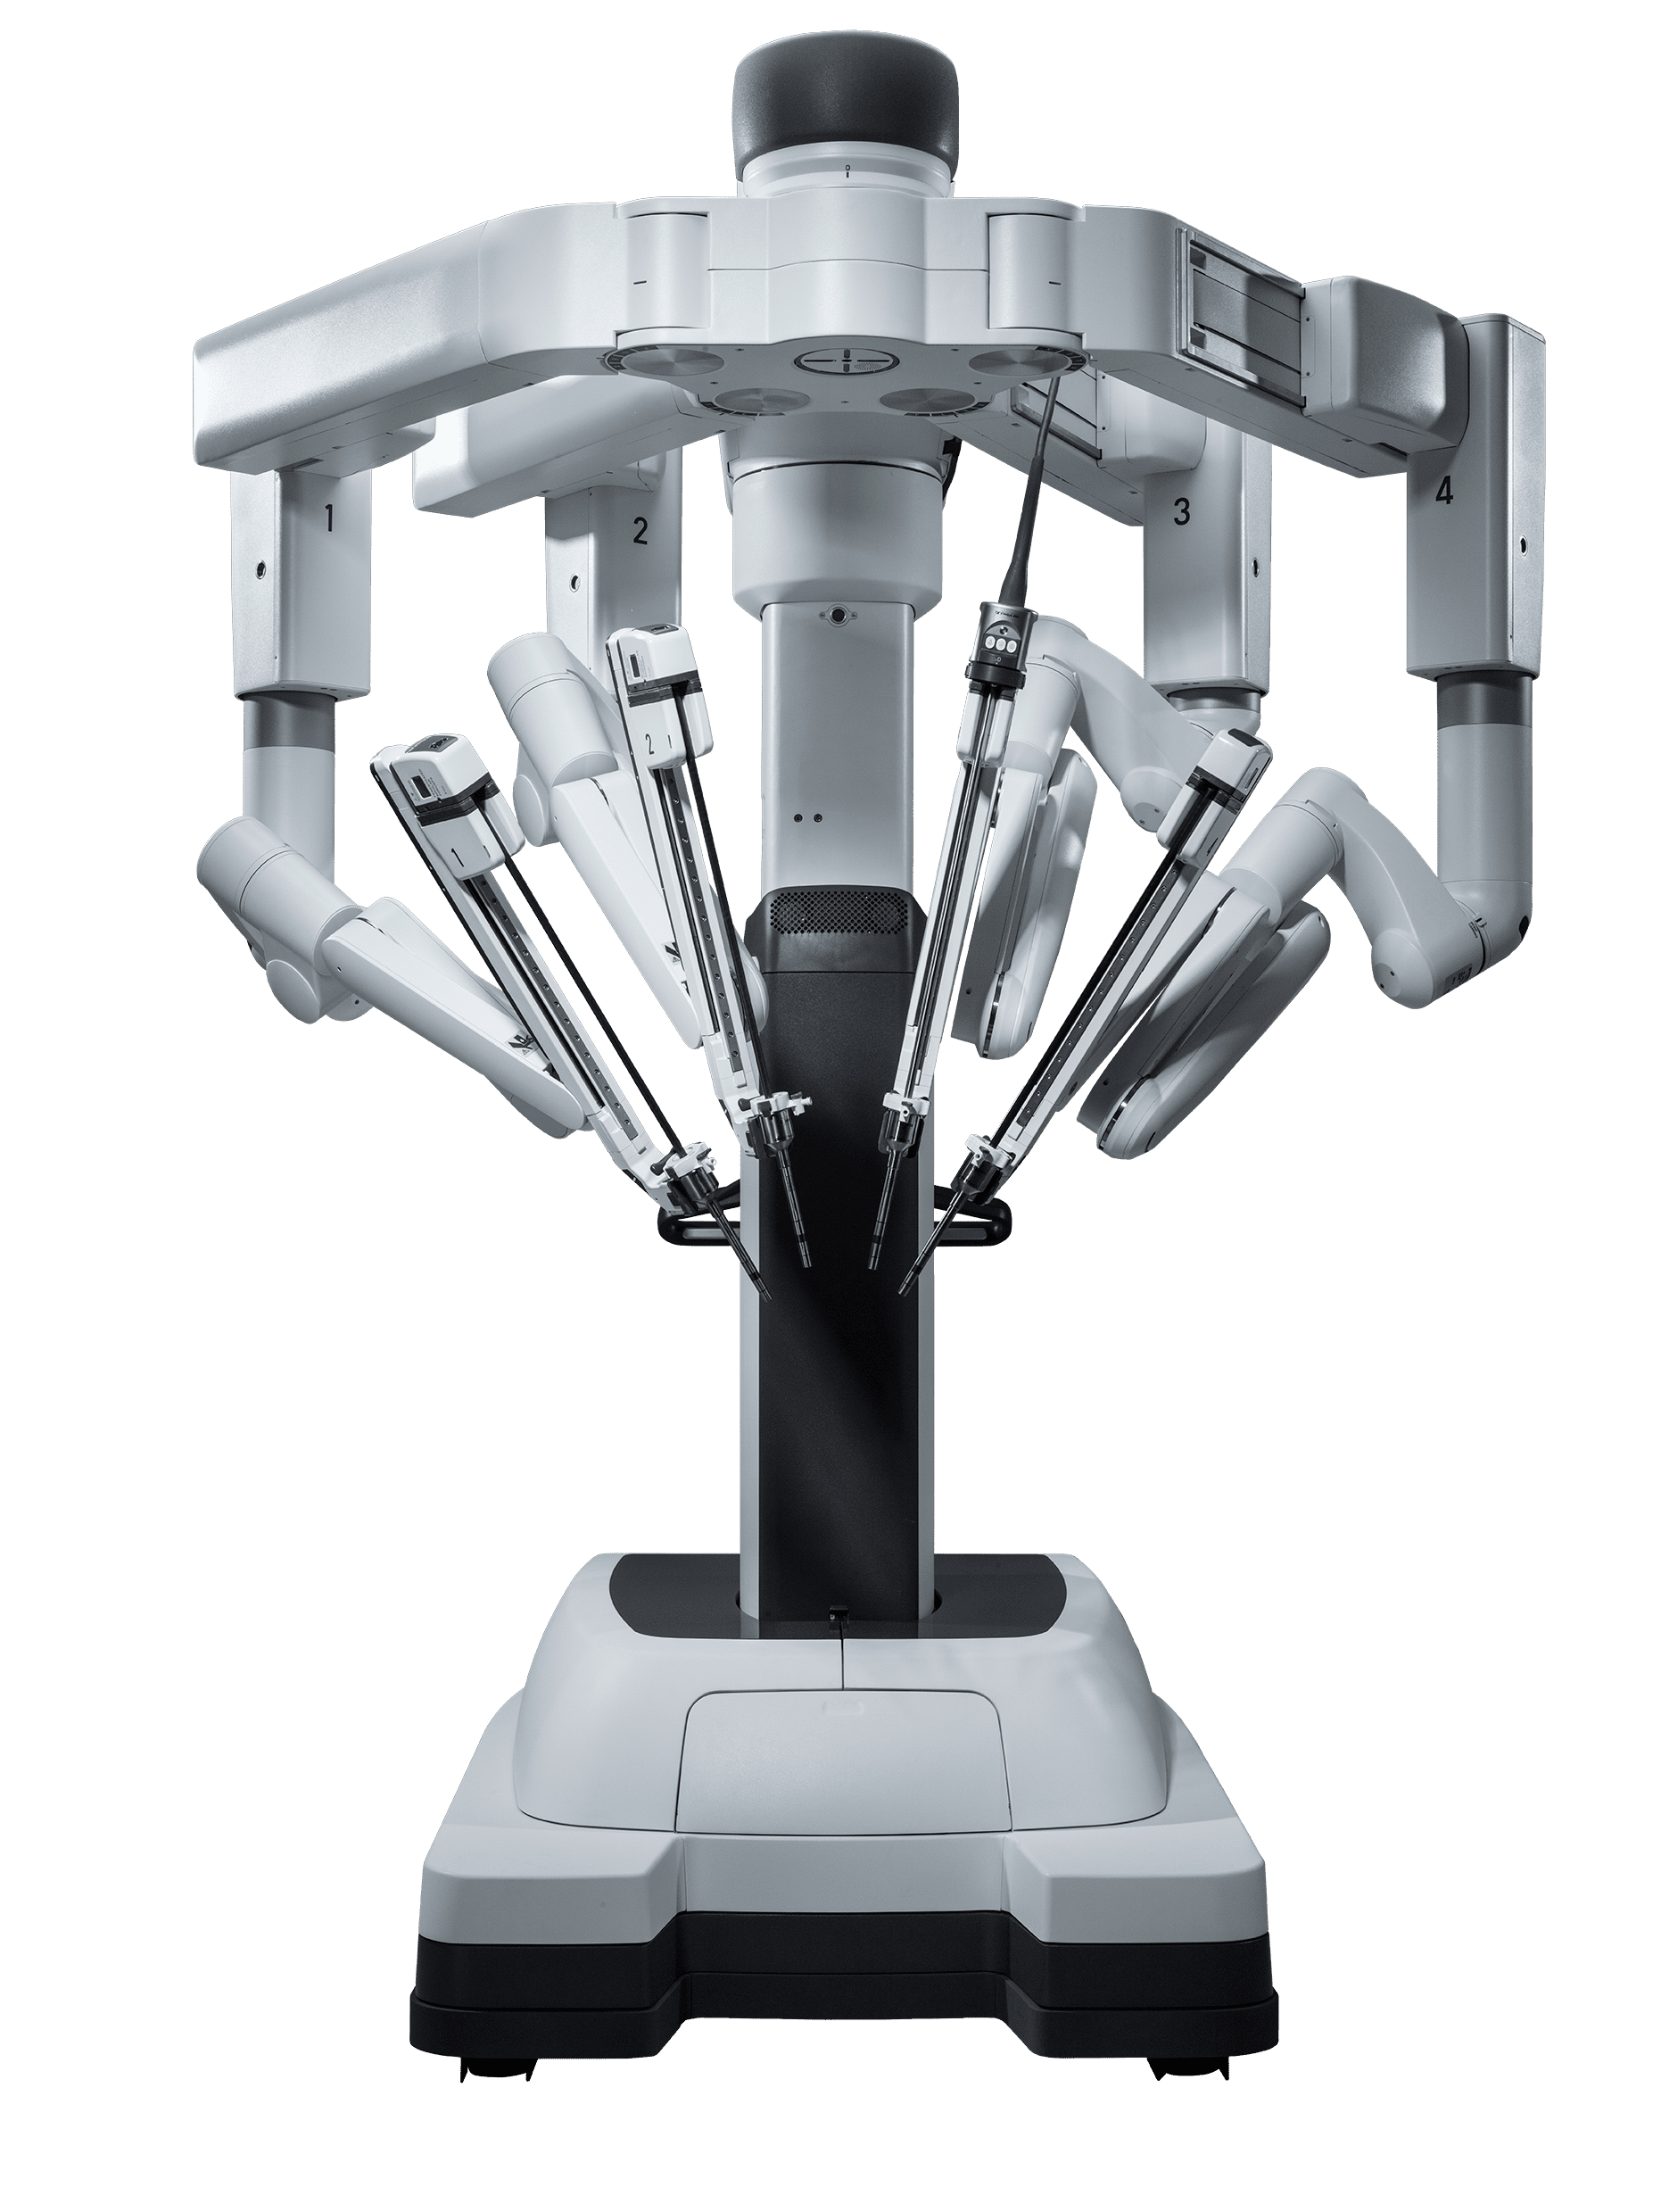
\includegraphics[width=9cm]{images/davinci-xi-patient-cart.png}\\
\caption{DaVinci Xi Patient Cart}
\end{figure}
\end{center}

Surgical robotics have a huge impact in Medicine and Healthcare in general. Some of the advantages are the following:
\begin{itemize}
\item \textbf{Minimally Invasive Procedures} which means
	\begin{itemize}
	\item Smaller incisions
	\item Less blood loss
	\item Reduced risk of inpatient infection
	\item Less pain
	\item Faster patient recovery
	\end{itemize}
\item Increased \textbf{precision} and reduced human errors
	\begin{itemize}
	\item Smooth and precise movements
	\item Detection and correction of errors caused by hand tremble
	\end{itemize}
\item \textbf{No fulcrum effect} and intuitive manipulation of surgical tools
\item \textbf{Haptic feedback}
\item \textbf{Teleoperation} (currently in the same room only): the surgeon operates while they sit on a special \textbf{ergonomic} console, which makes 
the long procedures more comfortable and efficient.
\end{itemize} 

\begin{center}
\begin{figure}[H]
\centering
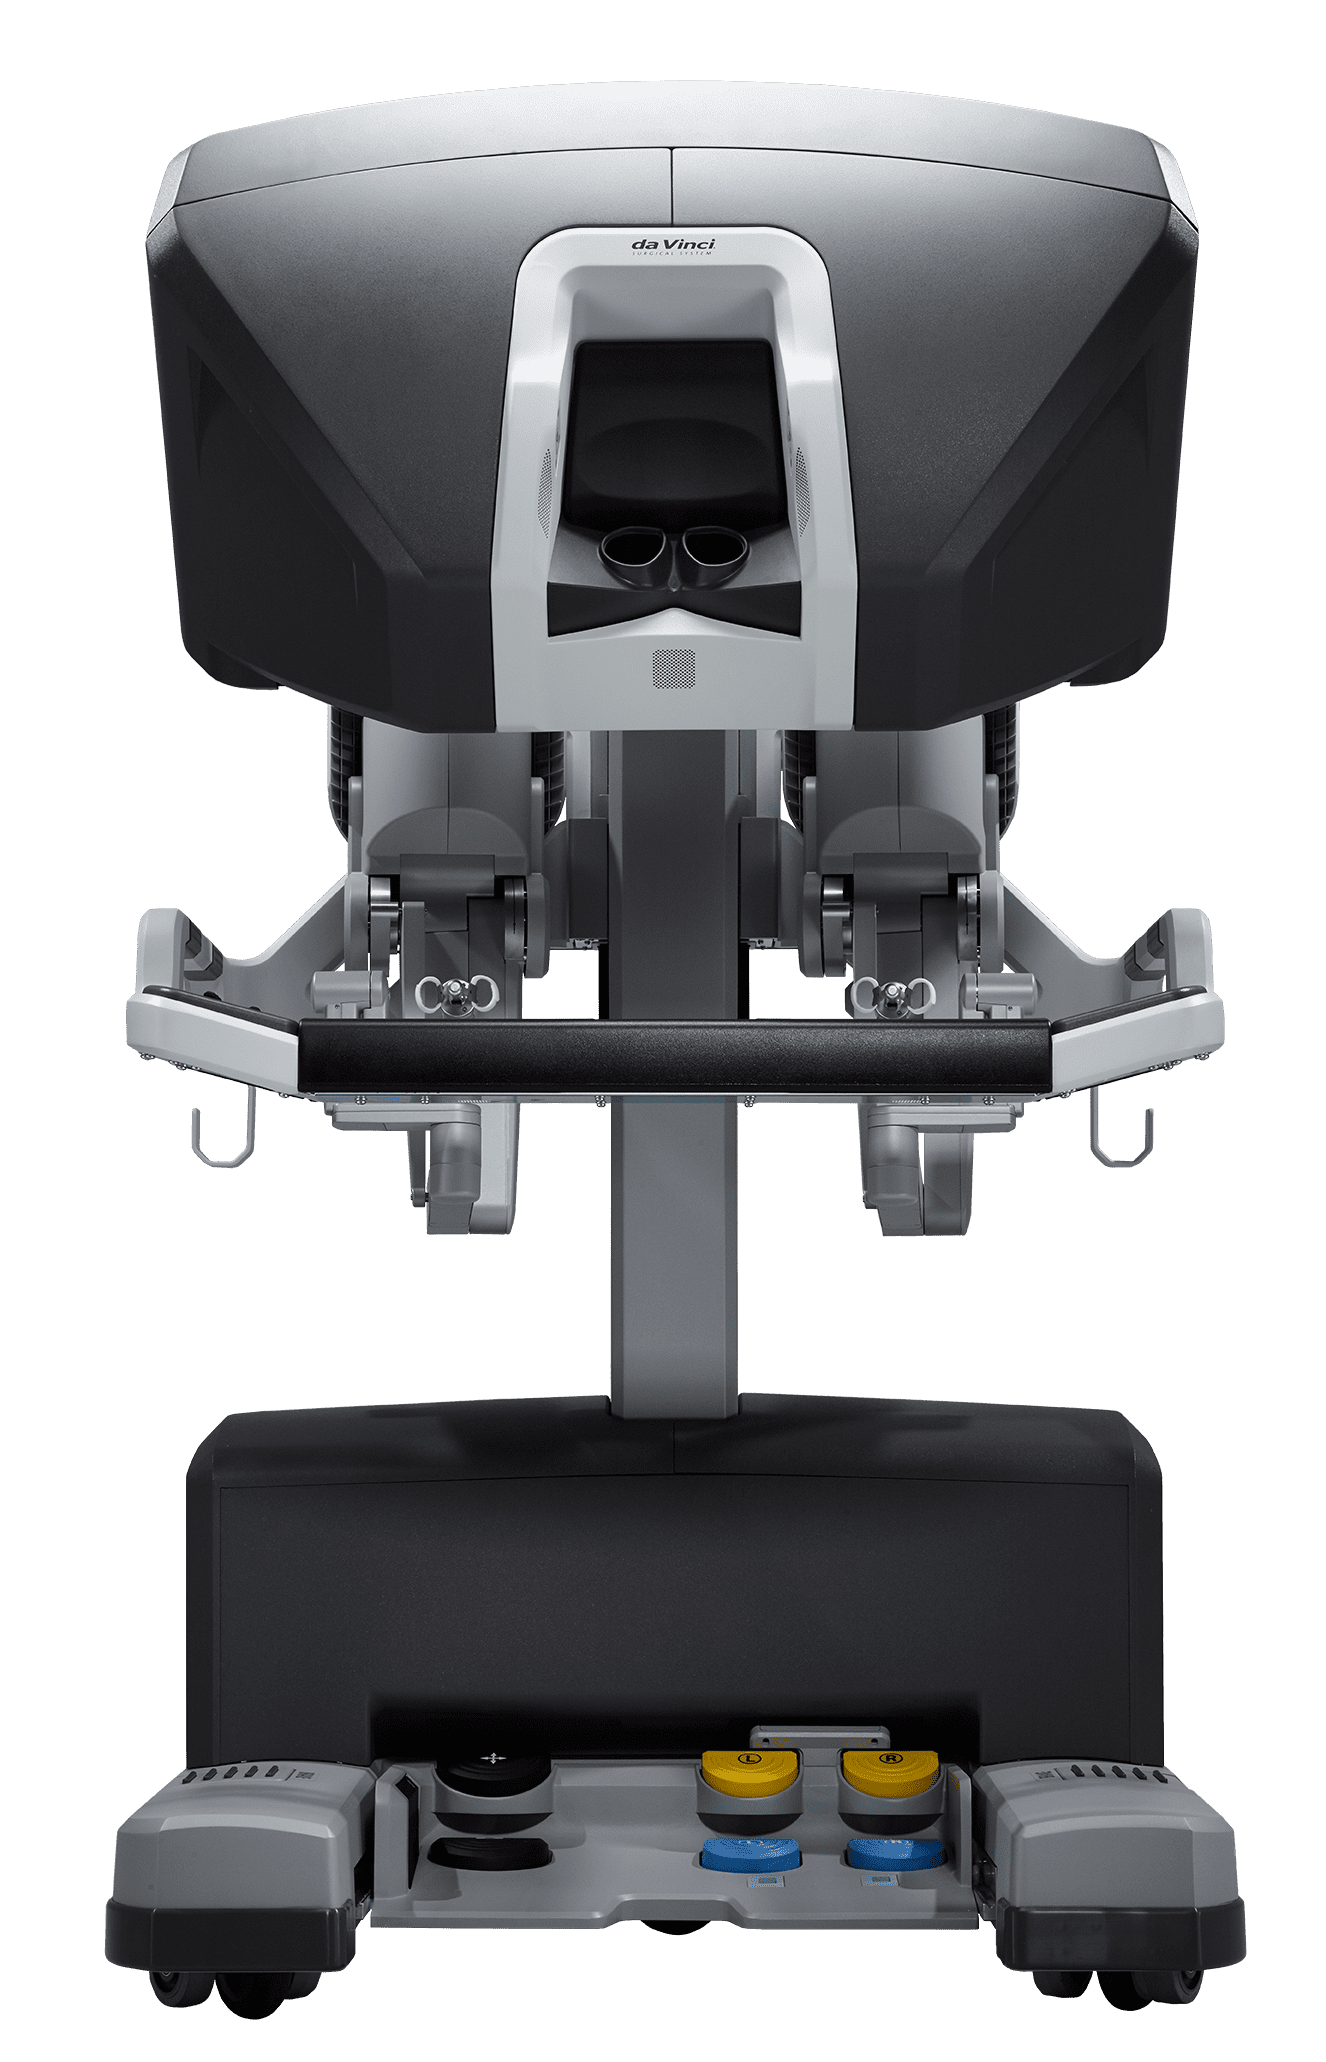
\includegraphics[width=7cm]{images/davinci-xi-surgeon-console.png}\\
\caption{DaVinci Xi Surgeon Console}
\end{figure}
\end{center}

\subsection{Bibliography Overview}

\subsection{Methodology \& Approach}

%\newpage
\section{Robotic arm Kinematic Analysis}


\subsection{Robotic arm, DH parameters \& Forward Kinematics}

\begin{center}
\begin{figure}[H]
\centering
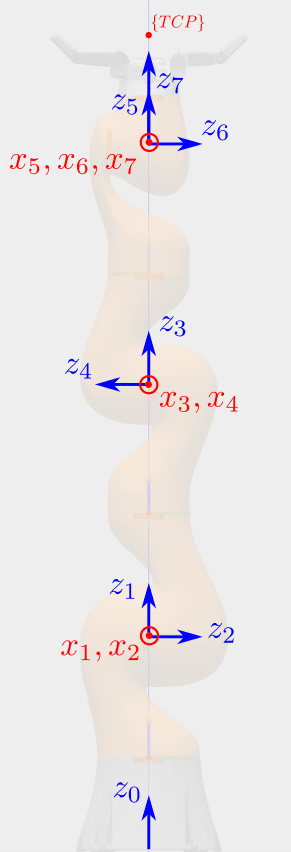
\includegraphics[height=12cm]{images/iiwa-frames.png}\\
\caption{Joint reference frames of the KUKA iiwa14 robot}
\end{figure}
\end{center}

\begin{center}
\begin{tabular}{ |c|c|c|c|c| } 
\hline
i & $θ_i$ (rad) & $L_{i-1}$ (m) & $d_i$ (m) & $α_{i-1}$ (rad) \\
\hline
1 & $θ_1$ & 0 & 0.36 & 0 \\
2 & $θ_2$ & 0 & 0 & $-π/2$ \\
3 & $θ_3$ & 0 & 0.36 & $π/2$ \\
4 & $θ_4$ & 0 & 0 & $π/2$\\
5 & $θ_5$ & 0 & 0.4 & $-π/2$ \\
6 & $θ_6$ & 0 & 0 & $-π/2$ \\
7 & $θ_7$ & 0 & 0 & $π/2$ \\
\hline
\end{tabular}
\end{center}

\[
^{i-1}T_i = 
\begin{bmatrix}
c\theta_i & -s\theta_i & 0 & L_{i-1} \\
s\theta_ica_{i-1} & c\theta_ica_{i-1} & -sa_{i-1} & -sa_{i-1}d_i \\
s\theta_isa_{i-1} & c\theta_isa_{i-1} & ca_{i-1} & ca_{i-1}d_i \\
0 & 0 & 0 & 1\\
\end{bmatrix}
\]


\subsection{Inverse Kinematics}

\subsubsection{Decoupling Technique}

In this section the inverse kinematics problem is solved for only the 6 out of the 7 total degrees of freedom. The third joint is not used in this 
analysis and it's angle is set to zero $θ_3 = 0$ . The rest of the joints form a special kind of kinematic chain that can be solved using the 
decoupling technique. In this technique the Inverse kinematics problem is split to 2 separate subproblems, one for the position and one for the 
orientation of the end-effector. This technique can be applied in this case because the axes of the 3 last joints intersect at the same point and 
they form an Euler wrist. \\

To solve for the joints' angles, the transformation matrix $^0T_7$ of the end-effector with respect to the robot's base is required. Usually the transformation ${}^UT_{tcp}$ is known, which is the pose of Tool's center point (TCP) with respect to the Universal Coordinate Frame $\lbrace U \rbrace$ from which the required $^0T_7$ can be calculated

\[
{}^UT_{tcp} = {}^UT_0  \;\;  {}^0T_7  \;\;   {}^7T_{tcp}
\]
\[
{}^0T_7 = {}^UT_0^{-1}  \;\;  {}^UT_{tcp}  \;\;  {}^7T_{tcp}^{-1}
\]
\[
{}^0T_7 = \begin{bmatrix}
R_t & \mathbf{p}_t \\
0 & 1 \\
\end{bmatrix}
\]

where ${}^UT_0,  \;\;   {}^7T_{tcp}$ are translation transformations by a constant distance and $R_t,  \;\; \mathbf{p}_t$ are the target's orientation 
and position respectively.

\[
{}^0\mathbf{p}_5 = {}^0T_4 {}^4\mathbf{p}_5 = \begin{bmatrix} p_x \\ p_y \\ p_z \\ \end{bmatrix}
\]

\begin{equation}
θ_1 = 
\begin{cases}
atan2 \left( p_y, p_x \right) \\
π - atan2 \left( p_y, p_x \right)
\end{cases}
\end{equation}

\begin{center}
\begin{figure}[H]
\centering
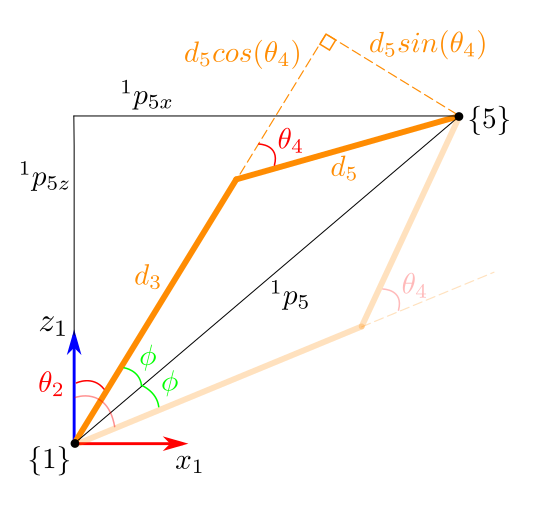
\includegraphics[width=8cm]{images/th2-4-calculation.png}\\
\caption{Calculation of angles $θ_2, θ_4$}
\end{figure}
\end{center}

\[
φ = acos \left( \frac{d_3^2 + \Vert{}^1p_{5}\Vert ^2 - d_5^2}{2d_3 \Vert{}^1p_{5}\Vert} \right)
\]
\begin{equation}
θ_2 = atan2 \left( \sqrt{p_x^2 + p_y^2}, {}^1p_{5z} \right) \pm φ
\end{equation}

\[ c_4 = \frac{ \Vert{}^1p_{5}\Vert ^2 - d_3^2 - d_5^2 }{2d_3d_5} \]
\begin{equation}
θ_4 = atan2 \left( \pm \sqrt{1 - c_4^2}, c_4 \right)
\end{equation}

Once $θ_1,θ_2,θ_3,θ_4$ are known, the orientation matrix of the wrist can be calculated as following
\[
R_{target} = 
\begin{bmatrix}
i_x & j_x & k_x\\
i_y & j_y & k_y\\
i_z & j_z & k_z\\
\end{bmatrix}
\]
\begin{equation}
θ_6 = atan2 \left( \pm \sqrt{1-k_y^2}, k_y \right)
\end{equation}
\[
θ_7 = atan2 \left( -j_y, i_y \right)
\]
\[
θ_5 = atan2 \left( - k_z, k_x \right)
\]


\subsubsection{Workspace constraints \& Singularity points}

\begin{center}
\begin{figure}[H]
\centering
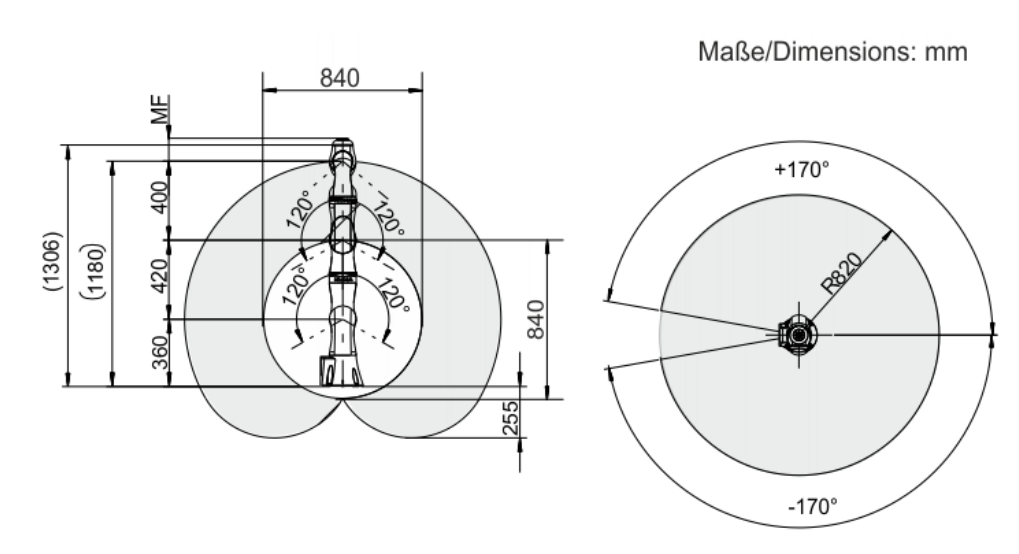
\includegraphics[width=10cm]{images/iiwa-workspace.png}\\
\caption{KUKA iiwa LBR14 workspace dimensions}
\end{figure}
\end{center}

Singularity points:
\begin{itemize}
	\item When $p_x^2 + p_y^2 = 0$ then the end-effector lies on the z-axis and $θ_1$ is not defined
	\item When $sin\left( θ_6 \right) = 0$ then the angles $θ_5, θ_7$ are not defined
\end{itemize}

\subsubsection{Solutions for 7DoF numerically}

\subsubsection{Comparison of Inverse Kinematics Techniques}


%\newpage
\section{Grasping}

\subsection{Gripper \& Forward Kinematics}

\begin{center}
\begin{figure}[H]
\centering
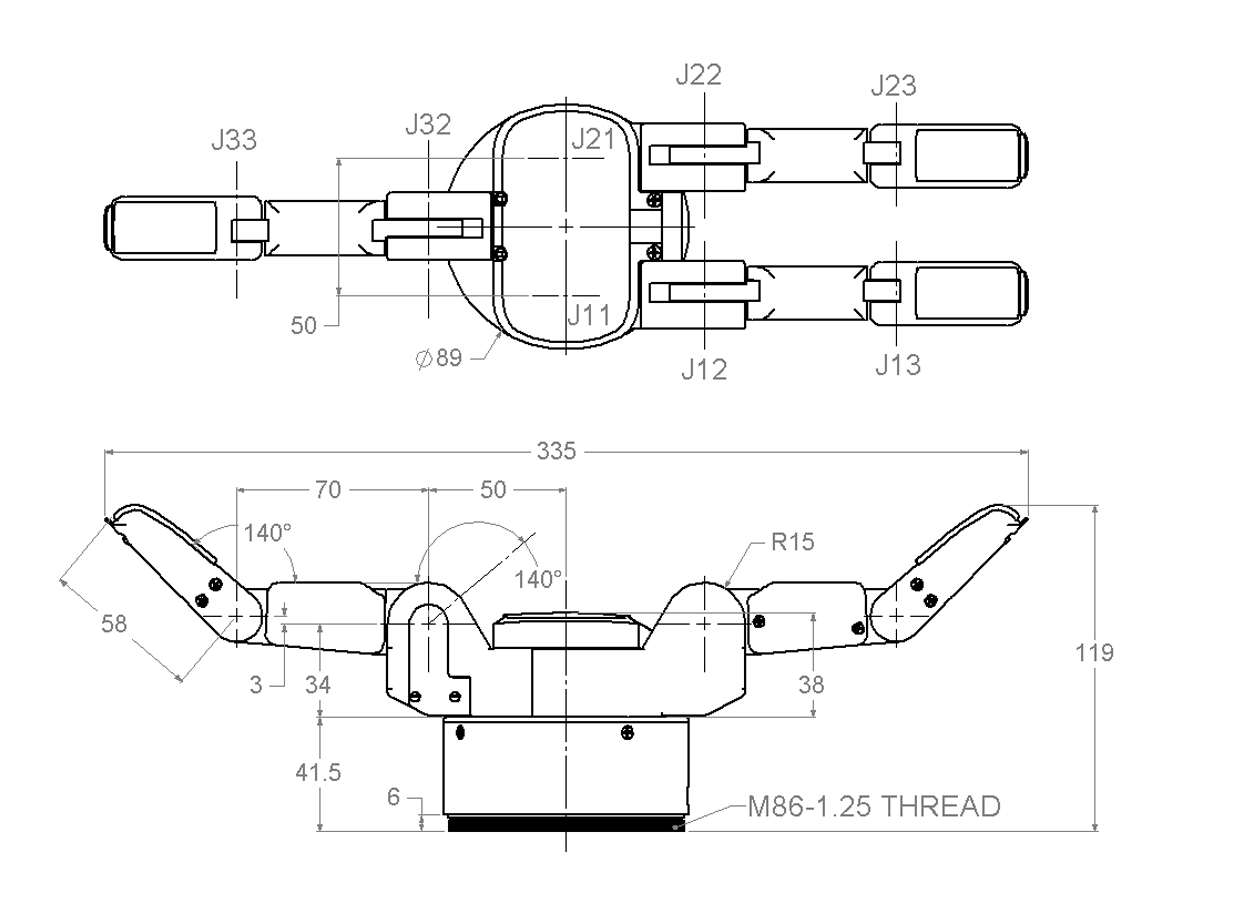
\includegraphics[width=12cm]{images/bh8-282-dimensions.png}\\
\caption{Barrett Hand gripper (model BH8-282) dimensions}
\end{figure}
\end{center}


\subsection{Gripper Inverse Kinematics}

The following Inverse Kinematics analysis referes to one finger of the Barrett Hand gripper, which has 3 revolute joints. Finger 3 has only 2 
revolute joints for which the angle solutions are the same with the solutions of the last 2 joints of the other fingers. Let

\[
\mathbf{p} = \begin{bmatrix} p_x \\ p_y \\ p_z \\ \end{bmatrix}
\]

be the position of the grasp point for one finger. The first angle can easily be calculated as

\begin{equation}
φ_1 = atan2 \left( p_y, p_x \right)
\end{equation}

Next, we calculate the third angle based on the law of cosines (see fig.)
\[
cos \left( π - φ_3 - \frac{π}{4} \right) = \frac{L_2^2 + L_3^2 - p^2}{2 L_2 L_3}
\]
\[
cos \left(φ_3 + \frac{π}{4} \right) = \frac{p^2 - L_2^2 - L_3^2}{2 L_2 L_3}
\]
\begin{equation}
φ_3 = atan2 \left[ \pm \sqrt{1 - \left( \frac{p^2 - L_2^2 - L_3^2}{2 L_2 L_3} \right)^2} , \frac{p^2 - L_2^2 - L_3^2}{2 L_2 L_3} \right] - \frac{π}{4}
\end{equation}

In a more general case, the first argument of the $atan2$ function in the expression of $φ_3$ could also be negative,
but in this case this second solution is rejected, because due to mechanical constraints, this angle can't be negative. 
After having calculated $φ_3$ we can calculate $φ_2 $

\[
tan \left( ψ + φ_2 \right) = \frac{p_z}{\sqrt{p_x^2 + p_y^2}}
\]
\[
tan \left( ψ \right) = \frac{L_3 sin \left( φ_3 + \frac{π}{4} \right) }{L_2 + L_3 cos \left( φ_3 + \frac{π}{4} \right)}
\]

\begin{equation}
φ_2 = atan2 \left( pz, \sqrt{p_x^2 + p_y^2} \right) - atan2 \left[ L_3 sin \left( φ_3 + \frac{π}{4} \right), L_2 + L_3 cos \left( φ_3 + \frac{π}{4} \right) \right]
\end{equation}

\subsection{Force closure}
The planar case, the spatial case \& convex hull test.

\lstinputlisting[frame=single,basicstyle=\ttfamily\small\color{blue},caption=Example ROS message with collision/contact information between one finger of the gripper and one surgical tool]{data/collision-contact-ros-message-example1.txt}

%\newpage
\section{Scene and object recognition with Computer Vision and Visual Servoing}

At this section we explore ways to detect and recognize the surgical tools as well as other objects of the simulation scene. To reduce the complexity of 
this thesis and focus on the more important features of this thesis, we assume in the simulation that the surgical tools are blue and the mounting dock, 
where the tools will be placed, is green. These assumptions make the scene and object recognition much easier without the need of more advanced image 
processing and/or machine learning recognition algorithms.\\

\textbf{Camera setup} used in this thesis:
\begin{itemize}
\item 2 HD RGB cameras with resolution $1280 \times 720$
\item near clipping plane: 0.02
\item far clipping plane: 300 
\item horizontal FoV (field of view): 1.396
\item update rate: 30fps
\end{itemize}

\subsection{Laparoscopic tool detection}

In order to detect the shape of the tool there are some standard steps that need to be executed. After having loaded the input image we convert it to grayscale, so that we can work on only one channel instead of
3 color channels and thus reduce the amount of calculations. Also for the purposes of extracting the shape of an object, the color doesn't have a very significant role in the algorithm. Next step is 
to remove the unwanted noise. In this thesis we only assume that the video frames have only Additive White Gaussian Noise (AWGN). To remove some of the
noise we use a moving average filter (the filter is also known as a kernel), which is convoluted around the whole image. The filter that was used is the following 3-by-3 matrix
\[
h = \frac{1}{9} \begin{bmatrix}
1 & 1 & 1 \\
1 & 1 & 1 \\
1 & 1 & 1 \\
\end{bmatrix}
\]
the output, filtered image is the result of the convolution of the image with the filter and is calculated as following
\[
g(i,j) = \sum_{k,l} f(i+k,j+l)h(k,l)
\]
where $g(\cdot, \cdot)$ is the output image and $f(\cdot, \cdot)$ is the input image.

After the noise is removed the image is getting binarized. To do that, we set a threshold, below which the pixels will be black and the rest will be white. This conversion to binary format, makes it 
easier to extract the boundaries of the black shapes, which will correspnd to the boundaries of the objects of the initial image.

\begin{center}
\begin{figure}[H]
\centering
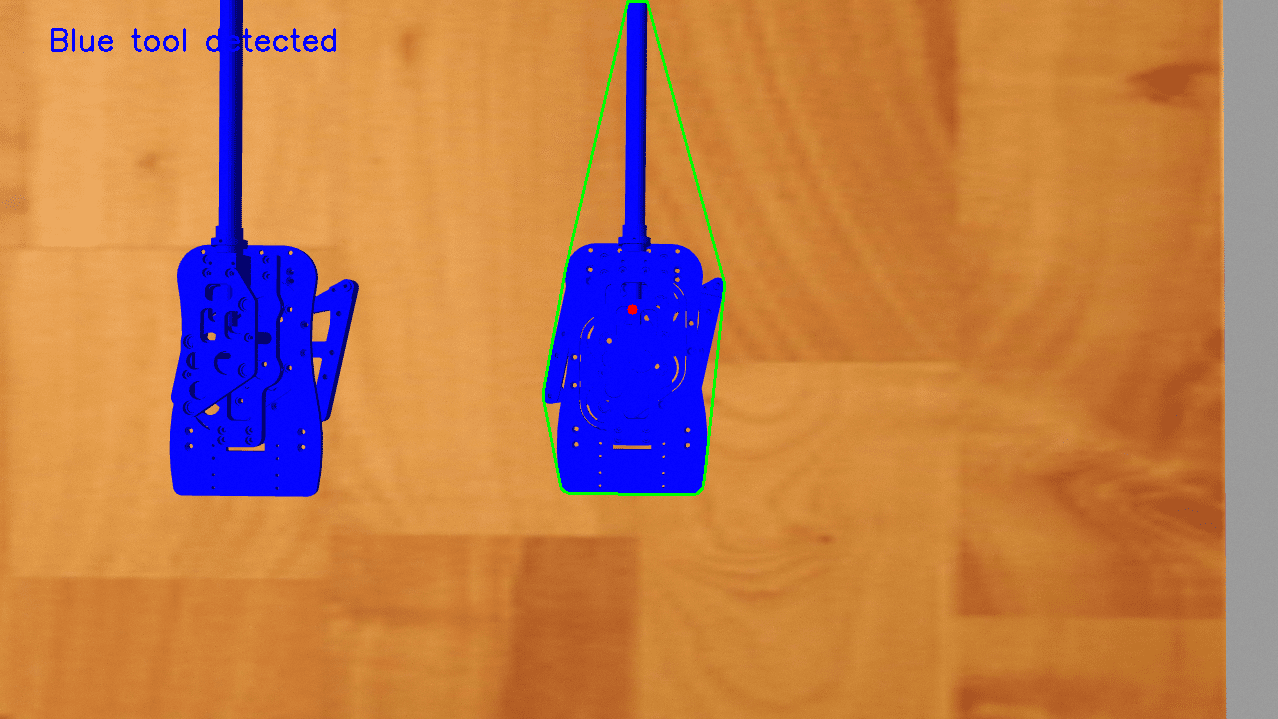
\includegraphics[width=12cm]{images/opencv-tool-convex-hull.png}\\
\caption{Simple tool detection in simulation based on color, using OpenCV. The green polygon is the convex hull, and the red point is the
estimated center of mass}
\end{figure}
\end{center}

\subsection{Stereoscopic vision}

\begin{center}
\begin{figure}[H]
\centering
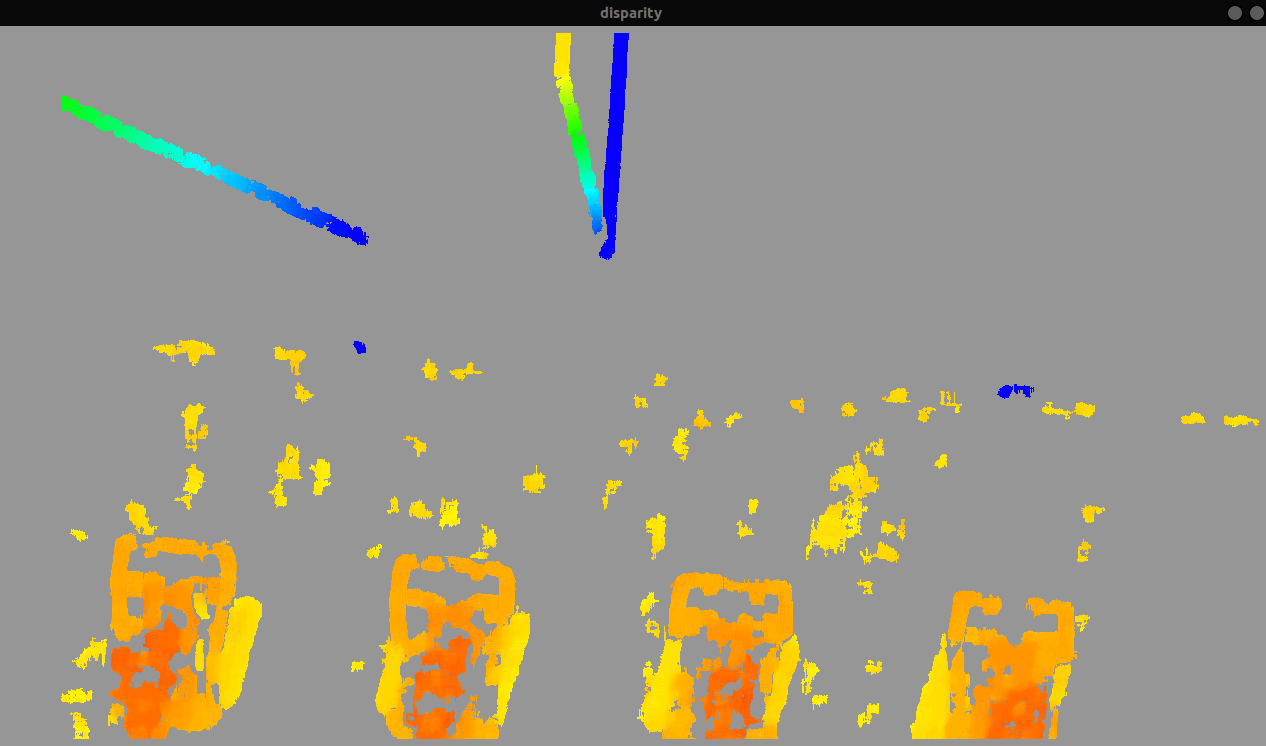
\includegraphics[width=12cm]{images/disparity.png}\\
\caption{Disparity image calculated from the 2 cameras}
\end{figure}
\end{center}

\begin{center}
\begin{figure}[H]
\centering
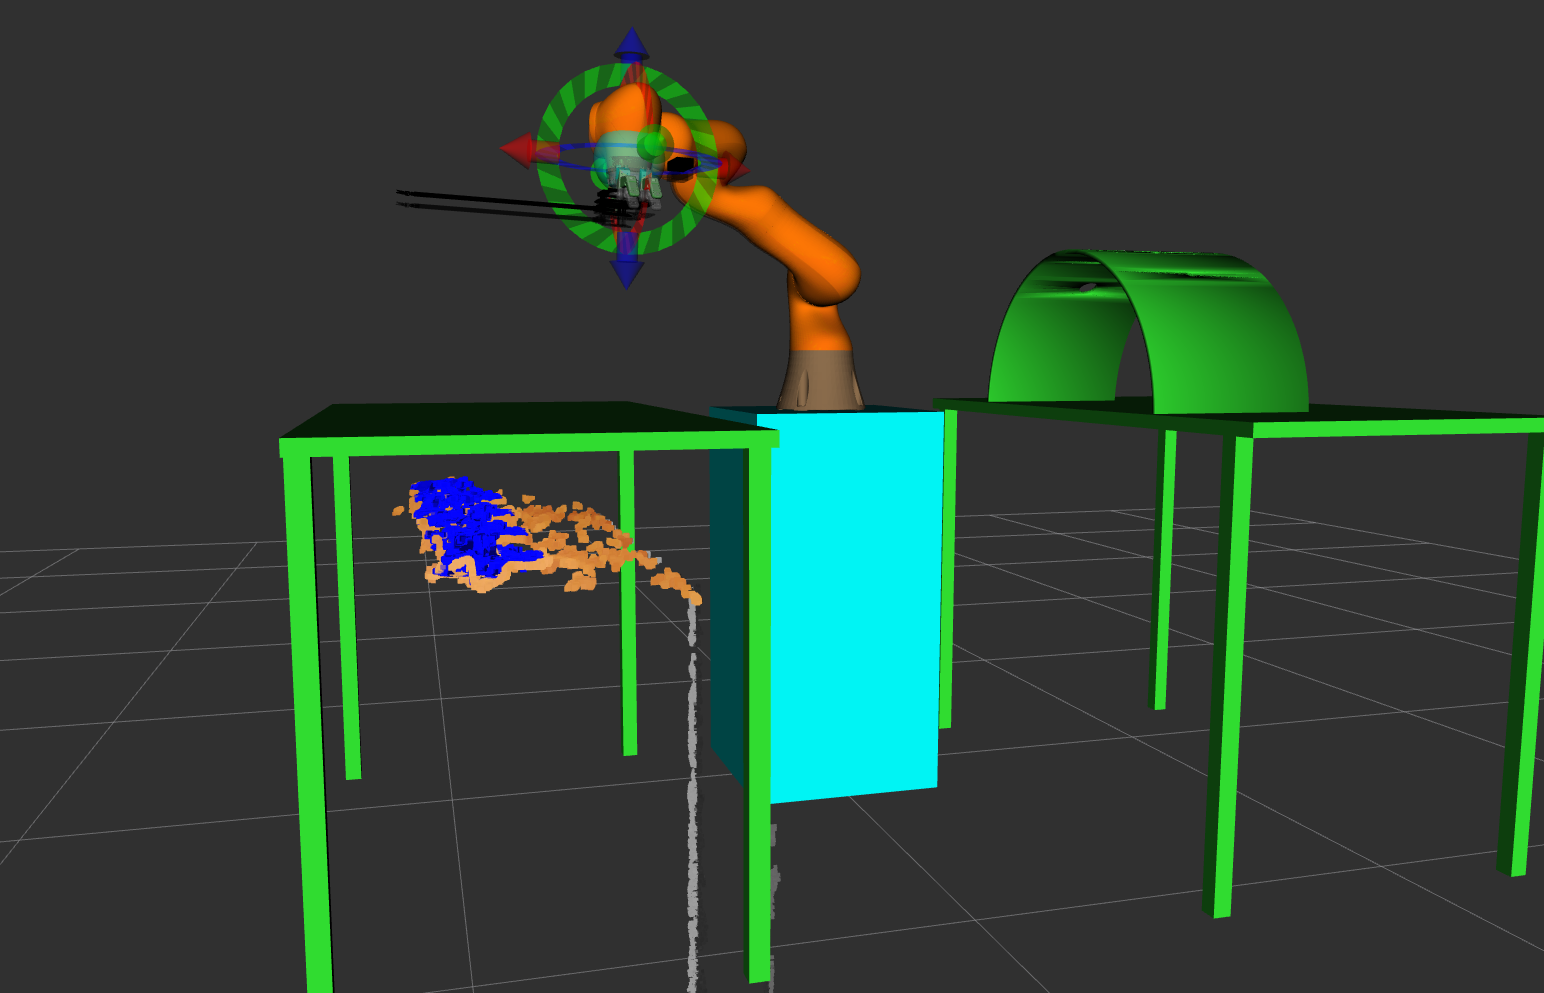
\includegraphics[width=12cm]{images/point_cloud.png}\\
\caption{Point cloud of surgical tools, generated from the 2 cameras and visualized in RViz}
\end{figure}
\end{center}

\subsection{Calculation of tool position and orientation}

In order for the gripper to grasp correctly the laparoscopic tool, it is required to calculate the tool's position and orientation in the pixel space 
which must then be converted with respect to the robot's workspace. From all the pixels that have been classified as part of the laparoscopic tool, 
one can estimate the center of mass and two perpendicular vectors 
attached to that point that define the orientation. The center of mass is simply the average of the $(x,y)$ coordinates of all the tool's pixels
\[
\left( \bar{x}, \bar{y} \right) = \left( \frac{1}{N}\sum_{i=1}^{N} x_i , \frac{1}{N}\sum_{i=1}^{N} y_i \right)
\]

The easiest way to calculate the center of mass is by calculating the average using the first moments of the contour points. However, since the contour is only using
the boundary of the object and not it's area, this method is not very accurate. To get a more accurate value for the center of mass, one must use the pixels that are inside 
the detected object's contour. The simplest way (but most expensive) to get the inside pixels of the tool is to loop over all the pixels and for each pixel check if it is inside the 
polygon (point inside polygon test). To make this method even faster, one can take a sample of the total pixels, for example check one in every 10 pixels in the x and y coordinates, 
which means reducing the time complexity to one tenth. \\

Taking this approach a step further in optimization, one can iterate not in all the video frame pixels but only those pixels 
that are inside the \textbf{Region of Interest} of the tool. The Region of Interest, also known as ROI, is a widely used structure in computer vision and is simply a bounding box (rectangle) that fits exactly 
(or is a bit bigger than) an object or part of the image frame that we want to study. Having already calculated the contour of the surgical tool and it's convex hull we can easily calculate this bounding box. 
For this calculation we prefer to use the convex hull, because it often contains much less pixels than the contour. We iterate over all the pixels of the convex hull and we get the minimum and maximum x and y 
coordinates. The combination of these four values is the desired ROI. Since we now have access to the tool's ROI, we can iterate and sample the pixels inside it (and not all pixels as we did before) to get 
some of the pixels of the tool so that we can more accurately calculate it's center of mass and orientation vectors. \\

The two orientation vectors are the eigenvectors of the covariance matrix of the above pixels. Let $\mathbf{a},\mathbf{b}$ be the orientation vectors, 
then $\mathbf{a},\mathbf{b}$ are solutions of the equation
\[
C \mathbf{v} = λ \mathbf{v}
\]
where $C$ is the covariance matrix given by
\[
C = \begin{bmatrix}
σ(x,x) & σ(x,y) \\
σ(y,x) & σ(y,y) \\
\end{bmatrix}
\]
\[
σ(x,y) = \frac{1}{n-1} \sum_{i=1}^{N} ( x_i - \bar{x} )( y_i - \bar{y} )
\]

\begin{center}
\begin{figure}[H]
\centering
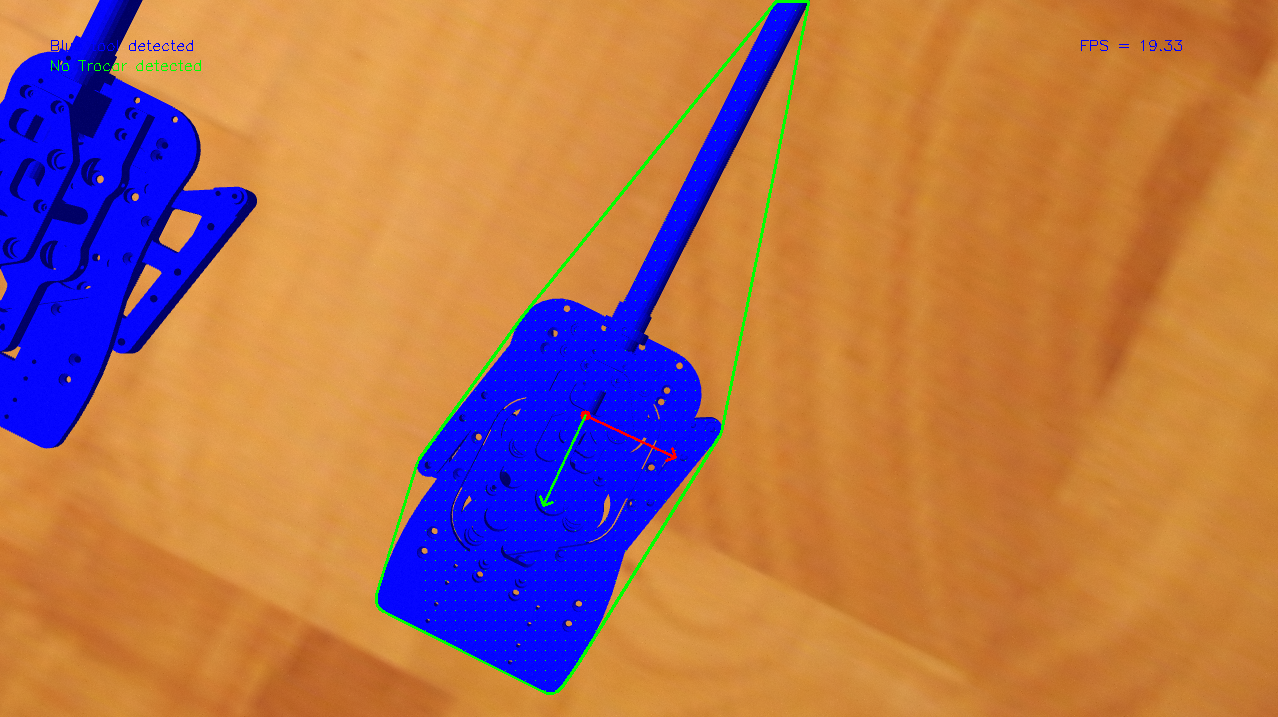
\includegraphics[width=0.8\textwidth]{images/tool-pose.png}\\
\caption{Estimation of tool's pose (position and orientation). The red dot is the center of mass and attached to that are the two orientation vectors of the tool. The green polygon is the convex hull of the tool 
and the white rectangle is it's ROI as calculated from the convex hull}
\end{figure}
\end{center}

\subsection{Calculation of grasping points}

\subsection{Trocar detection \& Estimation of fulcrum point}

\begin{center}
\begin{figure}[H]
\centering
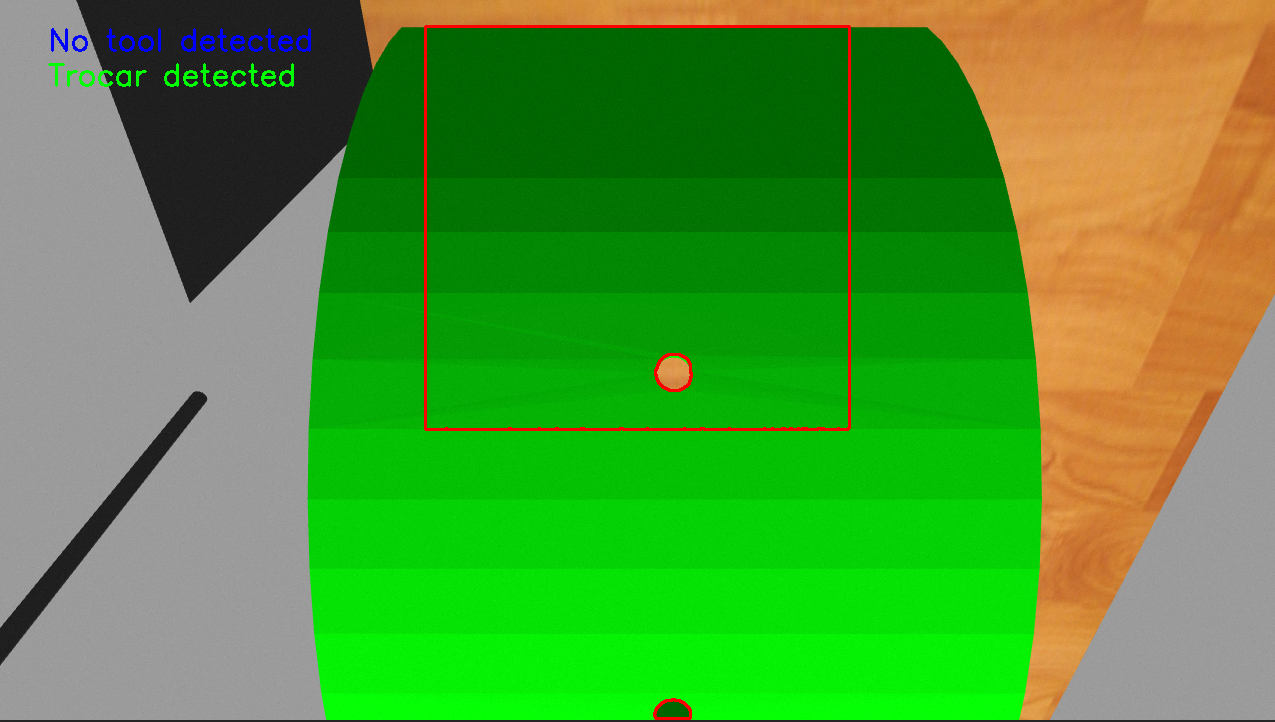
\includegraphics[width=12cm]{images/opencv-trocar-detection.png}\\
\caption{Simple trocar detection in simulation based on color, using OpenCV. In simulation, the trocar is simply considered to be a small 
cylindrical hole and it's center is the fulcrum point}
\end{figure}
\end{center}

\subsection{Visual Servoing}

At this chapter we briefly investigate how visual servoing can be applied in surgery robotics. \textbf{Visual Servoing} is the use of visual information 
to guide and control a robot. The main task of visual servoing is to control the end-effector's pose using features extracted from visual information. The 
features that are usually extracted from cameras are the position and orientation of the detected object, the distance of the object from the camera (using 
stereoscopic vision, photogrammetry or other techniques), the size and the shape of the object. The visual servoing can be executed either in the robot's space 
using position-based servoing or in the camera's space (also known as "pixel space") by using the image-based technique.

\subsubsection{Position based servoing}

\begin{center}
\begin{figure}[H]
\centering
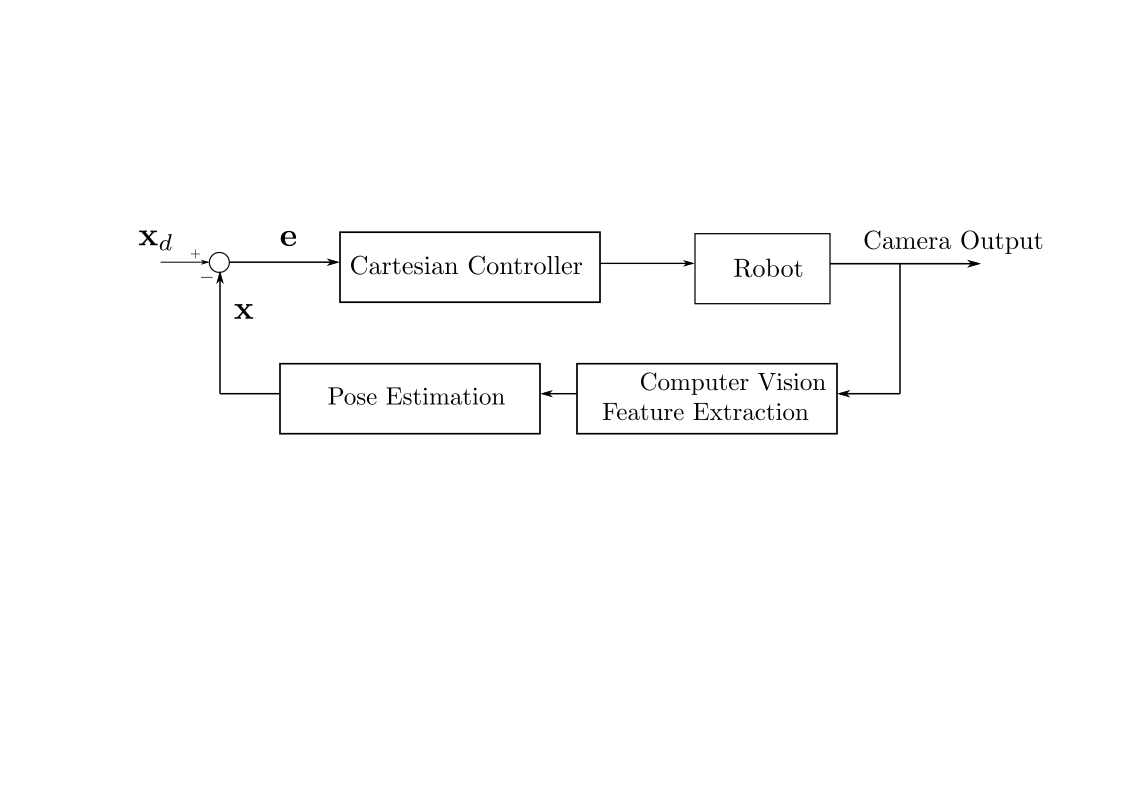
\includegraphics[width=0.8\textwidth]{images/visual-servoing-position-based.png}\\
\caption{Position based visual servoing closed loop control}
\end{figure}
\end{center}

\begin{itemize}
\item \textbf{Photogrammetric technique}
\item \textbf{Stereoscopic vision}
\item \textbf{Extracting depth from motion}
\end{itemize}

\subsubsection{Image based servoing}

\begin{center}
\begin{figure}[H]
\centering

\includegraphics[width=0.8\textwidth]{images/visual-servoing-image-based.png}\\
\caption{Image based visual servoing closed loop control}
\end{figure}
\end{center}

\begin{center}
\begin{figure}[H]
\centering
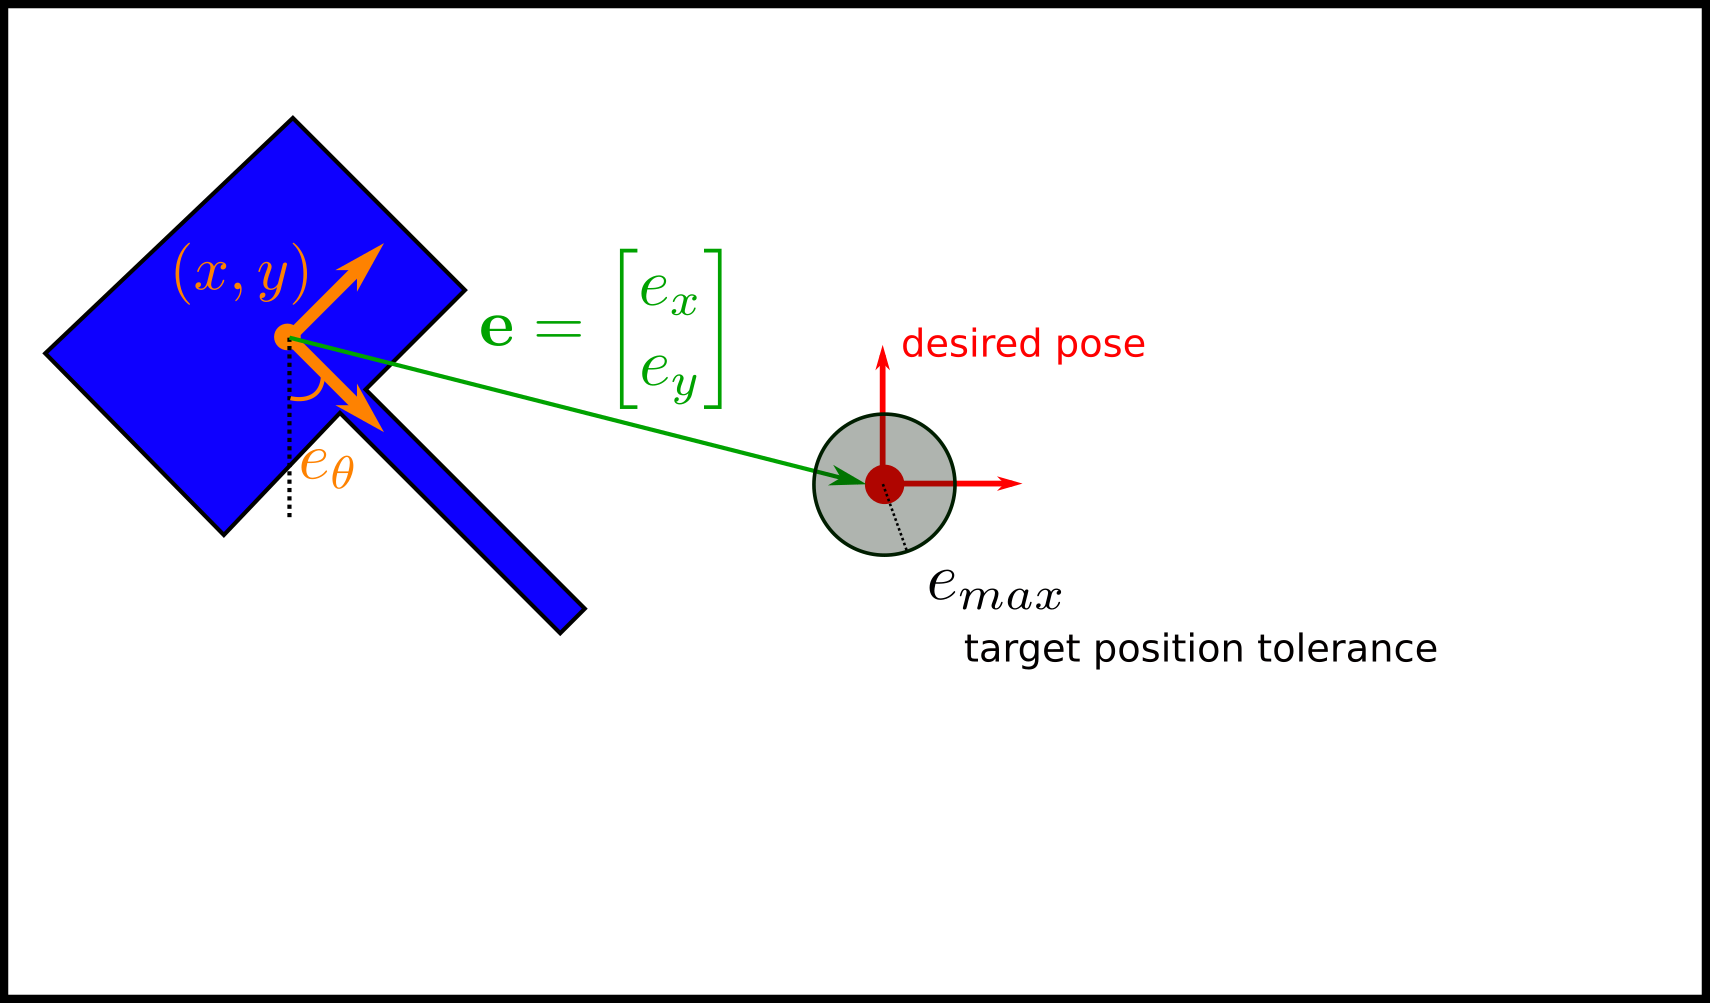
\includegraphics[width=0.45\textwidth]{images/visual_servo_start.png}
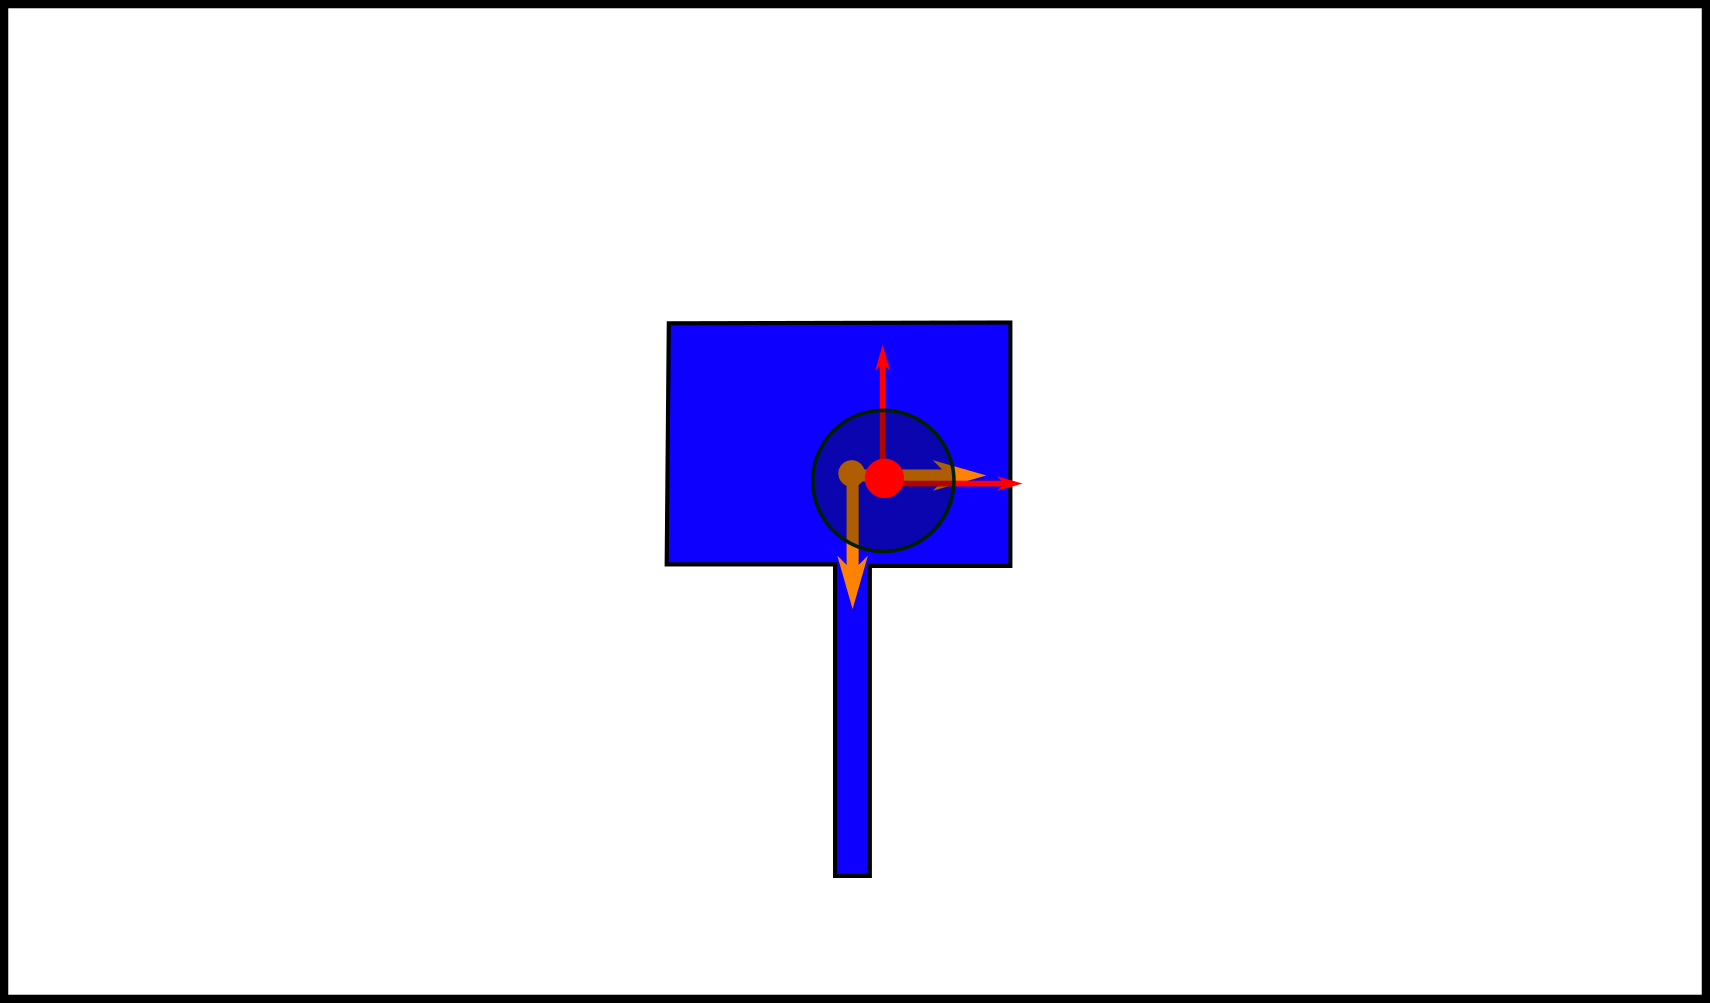
\includegraphics[width=0.45\textwidth]{images/visual_servo_end.png}\\
\caption{Image based visual servoing. The robot arm is controlled using the information gained from the video frames. The frames are 2Dimensional and thus 
the detected objects can have only 3 degrees of freedom which means we can mainly control 3 independent variables, here the $x,y,θ$ variables. The left image 
is the initial frame and the right image is the frame where the object is at the target pose.}
\end{figure}
\end{center}


%\newpage
\chapter{Path Planning}

\textbf{Path Planning} is a geometric problem, where it is desired to find a path from a starting point to a goal point and also satisfying a set of constraints, such as: 
restricting the solutions inside the robot's configuration space, avoiding obstacles in the task space, avoiding singularity points and respecting the robot's 
joint limits.


\section{Sampling methods}

The path planning algorithms that were mostly used in this thesis belong to the category of sampling methods. These methods use random functions to choose a sample from 
the configuration space or the state space. Sampling methods differ from the deterministic grid methods which, which discretize the whole space. Sampling methods are less 
computationally expensive than the grid methods, but they do not deliver optimal solutions like the latter.


\subsection{RRT Algorithms}

The \textbf{Rapidly-exploring Random Trees} algorithm is a sampling planning method that searches for an obstacle-free motion plan from an initial state $x_{init}$ to a set of goal states $\mathcal{X}_{goal}$. We refer to a set 
of goal states, because apart from the one desired goal state there can be other neighbor states that are within the allowed position and orientation tolerances.

\begin{algorithm}[H]
\SetAlgoLined
\ForEach{replanning attempt}{
	initialize vertices $V \leftarrow \lbrace x_{init} \rbrace$\;
	initialize edges $E \leftarrow \varnothing$\;
	initialize search tree $T \leftarrow (V,E)$\;
	\While{$time \leq maxPlanningTime$}{
		$x_{rand} \leftarrow$ getSampleStateFrom($\mathcal{X}$)\;
		$x_{nearest} \leftarrow$ getNearestNodeInTreeToState($T, x_{rand}$)\;
		$x_{new} \leftarrow$ findLocalPlanFromTo($x_{nearest}, x_{rand}$)\;
		\If{isPathCollisionFree($x_{nearest}, x_{rand}$)}{
			$V \leftarrow V \cup \lbrace x_{new} \rbrace $\;
			$E \leftarrow E \cup \lbrace (x_{nearest}, x_{rand}) \rbrace $\;
			\If{$x_{new} \in \mathcal{X}_{goal}$}{
				\Return SUCCESS and path plan $ T=(V,E) $ \;
			}
		}
	}
}
\Return FAILURE and $ T=(V,E) $ \;
\caption{RRT Algorithm}
\end{algorithm}

Other variations of the RRT Algorithm, which are also available in the OMPL library, included in the MoveIt library of ROS framework  are:
\begin{itemize}
	\item \textbf{TRRT} Transition-based RRT
	\item \textbf{BiTRRT} Bidirectional Transition-based RRT
	\item \textbf{RRT*}
	\item \textbf{RRTConnect} with is the default OMPL path planner in ROS
	\item \textbf{LBTRRT} Lower Bound Tree RRT
\end{itemize}


\subsection{PRM Algorithms}

The \textbf{Probabilistic Roadmap} (PRM) algorithm is a sampling planning method that constructs a roadmap representation of $\mathcal{C}_{free}$ \textbf{before searching} for a solution. After the roadmap is successfully built, then the algorithm searches 
for a solution using a traditional graph-based search algorithm. A very important aspect of this algorithm is how the sampling of the free configuration space will be done. The sampling is usually performed using a 
uniform distribution except from the regions close to objects where the sampling is more dense.

\begin{algorithm}[H]
\SetAlgoLined
initialize vertices $V \leftarrow \lbrace x_{init} \rbrace$\;
initialize edges $E \leftarrow \varnothing$\;
initialize roadmap graph $G \leftarrow (V,E)$\;
\For{$i = 1, \ldots , n$}{
	$x_{rand,i} \leftarrow$ getSampleStateFrom($\mathcal{X}$)\;
	$\mathcal{N}(x_{rand,i}) \leftarrow$ getKNearestNeighbors($G=(V,E), x_{rand,i}$)\;
	$V \leftarrow V \cup \lbrace x_{rand,i} \rbrace $\;
	\ForEach{$x \in \mathcal{N}(x_{rand,i})$}{
		\If{there is no edge between $x$ and $x_{rand,i}$}{
			\If{isPathCollisionFree($x_{nearest}, x_{rand,i}$)}{
				$E \leftarrow E \cup \lbrace (x_{rand,i}, x), (x, x_{rand,i}) \rbrace$
			}
		}
	}
}
\Return $G=(V,E)$
\caption{PRM roadmap construction (preprocessing phase)}
\end{algorithm}

Other variations of the PRM Algorithm, which are also available in the OMPL library, included in the MoveIt library of ROS framework  are:
\begin{itemize}
	\item \textbf{PRM*}
	\item \textbf{LazyPRM}
	\item \textbf{LazyPRM*}
\end{itemize}


\section{Pick and place algorithm}

% Help on using the algorithme package
% http://ftp.ntua.gr/mirror/ctan/macros/latex/contrib/algorithm2e/doc/algorithm2e.pdf 
\begin{algorithm}[H]
\SetAlgoLined
\ForEach{surgical tool}{
	\tcc{Plan the Pick pipeline}
	set grasp pose\;
	set pre-grasp approach\;
	set post-grasp retreat\;
	set posture of eef before grasp (open gripper)\;
	set posture of eef during grasp (closed gripper)\;
	\tcc{Plan the Place pipeline}
	set place location pose\;
	set pre-place approach\;
	set post-grasp retreat\;
	set posture of eef after placing object\;
	Plan pick and place paths\;
}
\caption{Pick and Place algorithm}
\end{algorithm}

If the pick and place algorithm targets small objects, such as cubes or spheres or other small convex objects then the path planning is straightforward. In the case where, the object to pick and place has at least one 
dimension that is bigger than the others like a rod or other long objects, such as the surgical tools, used in this thesis, then the path planning becomes more complicated, because of the almost certain collisions 
of the tool with the links of the rest of the robot (the link of the end-effector will probably not collide with the tool).


\section{Task space analysis}

Before designing any paths and trajectories it is very important to better understand the taskspace in which the surgical tool will operate in. When the robot arm is in the pick-and-place phase where it detexts the surgical 
tool and grasps and then go to the mounting dock to insert it, then at this phase, the taskspace is the same as the robot's taskspace. However, when the surgical tool is inserted in the patient's body and starts executing 
pivoting motions, then there are 2 taskspaces that are studied. The first one is the surgical taskspace, which is where the surgical movements are planned (sutures, laparoscopic camera movements etc.) and the second 
taskspace is the one outside of patient's body in which the planned paths are "mirrored" so that the robot can execute them. The surgical taspace $\mathbb{S}$ is the one shown in figure \ref{surgical-taskspace}. The paths inside 
the surgical task are transformed via the Fulcrum effect transformation, which is described in more detail in \ref{section:fulcrum-effect}, to the pivot paths taskspace $\mathbb{P}$ which is a subset of the robot's taskspace 
$\mathbb{T}$ (we assume that all pivot motions can be executed, i.e. that all motions are reachable and fully inside the robot's taskspace). The paths are then used as input to a trajectory generator whose output 
is transformed via the Inverse Kinematics equations to the joint angles that belong to the joint space $\mathbb{J}$. \\

Alternatively in a mathematical notation, the fulcrum effect transformation is notated as
\begin{equation}
Φ: \mathbb{S} \longrightarrow \mathbb{P}
\end{equation}
the inverse kinematics transformation is described as
\begin{equation}
IK: \mathbb{P} \subset \mathbb{T} \longrightarrow \mathbb{J}
\end{equation}
and similarly the forward kinematics transformation can be described as
\begin{equation}
FK: \mathbb{J} \longrightarrow \mathbb{T}
\end{equation}\\

\begin{center}
\begin{figure}[!htb]
\centering

\includegraphics[width=\textwidth]{images/spaces-and-transformations.png}\\
\caption{The spaces studied in this thesis and how they are connected with each other via transformations}
\label{surgical-taskspace}
\end{figure}
\end{center}

Having defined all the spaces, the Dexterity metric of the tool's task space (same as the surgical taskspace) can be defined as
\begin{equation}
\mathcal{D} = \mathcal{L}_q \mathcal{M}
\label{dexterity-measure}
\end{equation}
where
\begin{equation}
\mathcal{M} = \sqrt{det(J J^\top)}
\end{equation}
\begin{equation}
\label{joint-limit-measure}
\mathcal{L}_{q}=1-\exp\left\{-\kappa\prod_{i=1}^{n_{k}}\frac{(q_{ {i}}-q_{i,\min})(q_{i,\max}-q_{i})}{(q_{i,\max}-q_{i,\min})^{2}}\right\}
\end{equation}

\begin{center}
\begin{figure}[!htb]
\centering
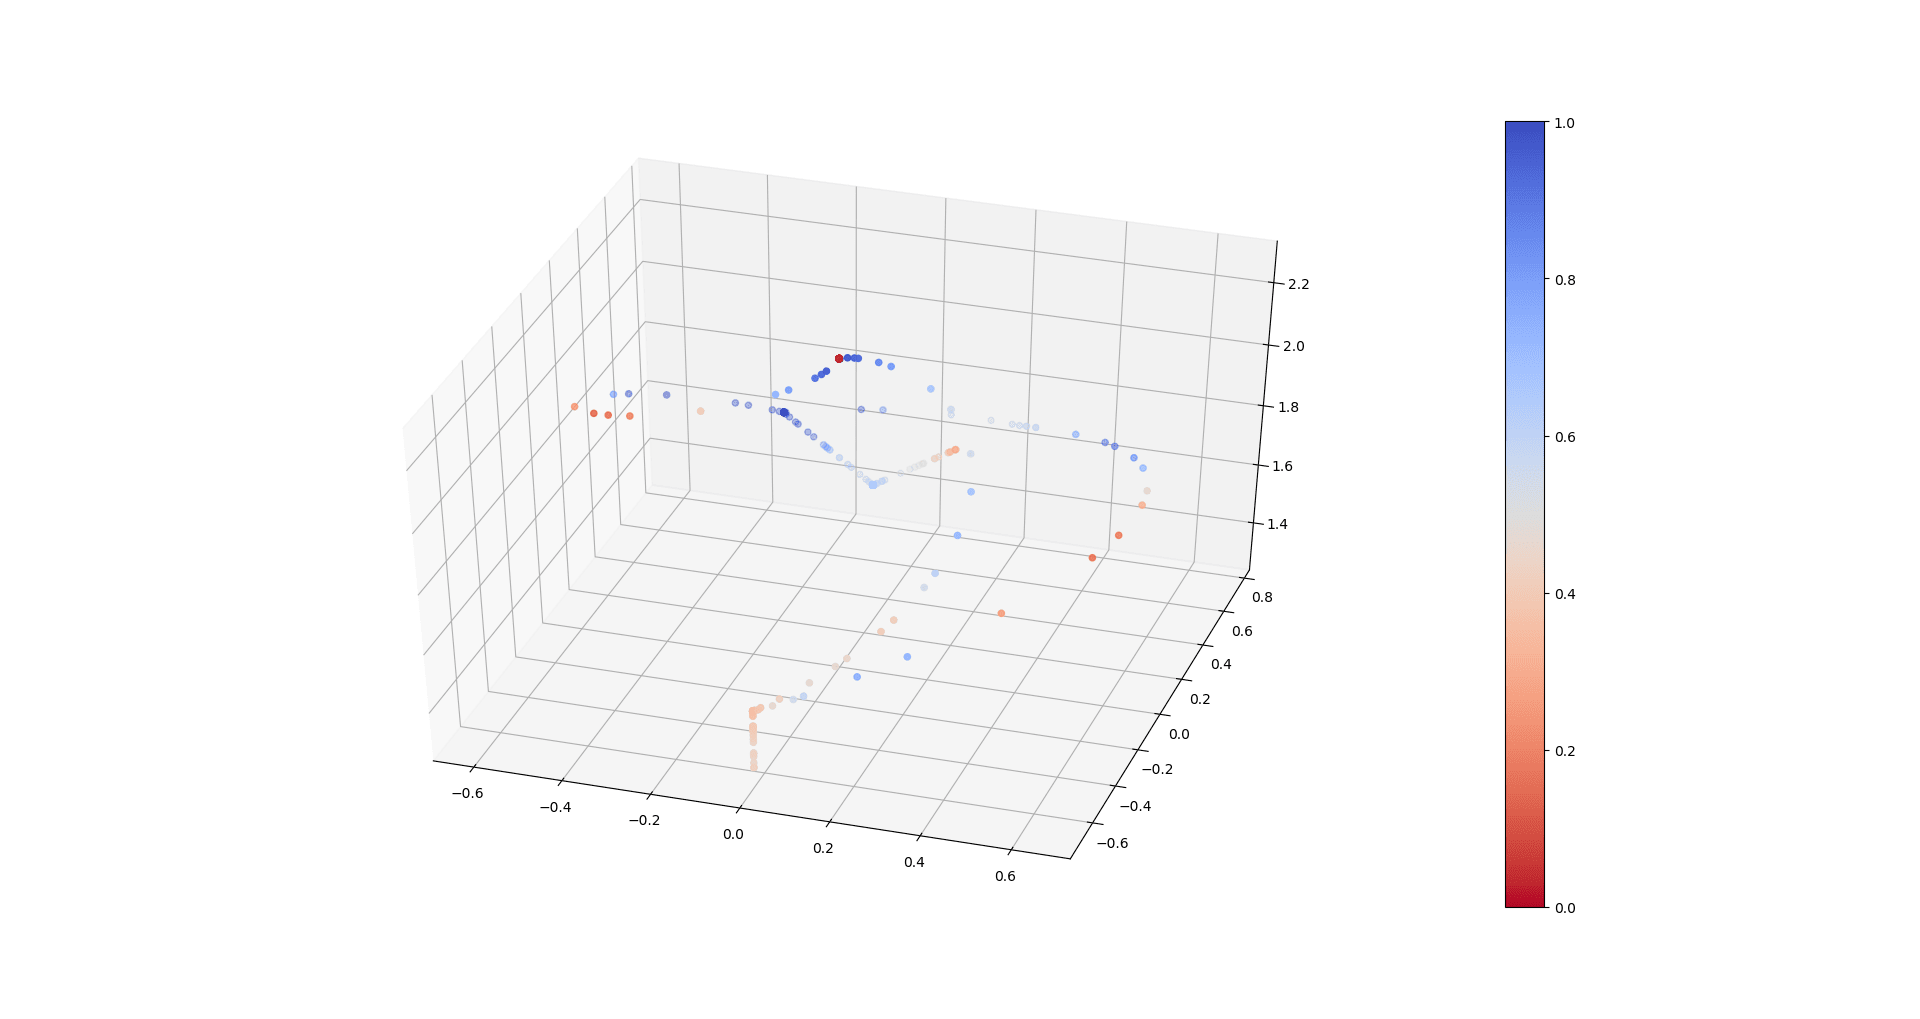
\includegraphics[width=10cm]{images/robot-planner1-manipulability-plot.png}\\
\caption{Plot the manipulability of the robot arm at sample points of the executed trajectory}
\end{figure}
\end{center}

The equation \ref{joint-limit-measure} calculates a joint limit measure which is multiplied with the manipulability measure and gives the dexterity measure.
From that equation we can conclude the following:
\begin{itemize}
\item If $q_i = q_{min}$ or $q_i = q_{max}$ then the exponential is equal to 1 which means that $\mathcal{L}_{q}$ and $\mathcal{D}$ are both 0, which means 
that the robot has \textbf{no dexterity at the boundary of the task space}.
\item If the value of $q_i$ is close to it's boundary value then the dexterity approaches 0. The how much close or far it is from the boundary (or in other words 
how fast the exponential term converges) depends on the parameter $\kappa$
\item The $q_{min}, q_{max}$ are calculated from the geometry of the task-space
\end{itemize}

For maximum dexterity at most points of a trajectory in a pivoting motion, the pivot sub-
taskspace (i.e. the space of all configurations of feasible pivot motions) must be fully within 
the robot’s whole reachable taskspace, otherwise only a small range of pivot movements will be 
feasible.\\

Finding $q_{i,min}, q_{i,max}$ at \ref{joint-limit-measure} is very difficult and time-consuming especially at task spaces with more intricate geometries. 
A similar and more practical equation to \ref{joint-limit-measure} can be written for calculating the dexterity of the robot in task space:

\begin{equation}
\label{rcm-taskspace-limit-measure}
\mathcal{L}_{p}=1-e^{-\kappa (r_{max} - r)}
\end{equation}
where $r_{max}$ is the maximum radius of a circle that the tool tip can follow at a given insertion depth $z$. Moreover, at every point of the taskspace, it is $L^2 = r^2 + z^2$. 
The equation \ref{rcm-taskspace-limit-measure} however only shows dexterity in terms of approaching the boundary of the taskspace and it does not take into consideration internal points of low 
dexterity and singularities like equation \ref{dexterity-measure}.

\begin{listing}[H]
\begin{minted}[tabsize=2,breaklines,frame=lines,framesep=2mm,baselinestretch=1.2,fontsize=\footnotesize, linenos]{matlab}
x = []; y = []; z = [];
r = [];
s = 0:0.005:0.5;
L = 0.48;
k = 4.5;

for z0=-L:0.01:0
    if abs(z0)*sqrt(2) <= L
        rmax = abs(z0);
    else
        rmax = sqrt(L^2-z0^2);
    end
    for r0=0:0.02:rmax
        x = [x, r0*cos(2*pi*s)];
        y = [y, r0*sin(2*pi*s)];
        z = [z, z0*ones(size(s))];
        lp = 1-exp(-k*(rmax-r0));
        r = [r, lp*ones(size(s))];
    end
end
\end{minted}
\caption{RCM Taskpace calculation using MATLAB}
\label{code:rcm_taskspace_matlab}
\end{listing}

\begin{center}
\begin{figure}[!htb]
\centering
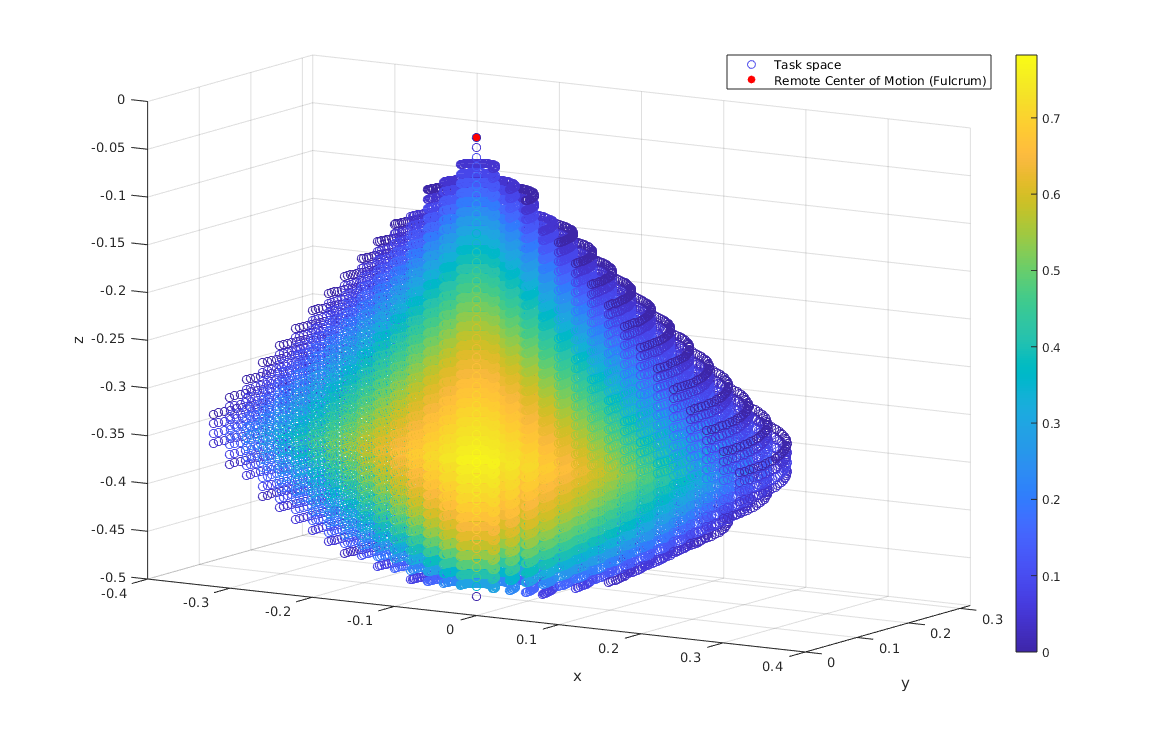
\includegraphics[width=0.8\textwidth]{images/rcm_taskspace.png}\\
\caption{Task space inside patients body. Colors with 0 or low value correspond to points with low dexterity. This is the trivial case, where no collision objects are taken into consideration}
\label{surgical-taskspace}
\end{figure}
\end{center}

All of the metrics above, measure how much reachable are various points of the surgical taskspace, but they are calculated from different perspectives, using input values from different spaces.
\begin{equation}
\mathcal{L}_{q}, \mathcal{M}: \mathbb{J} \longrightarrow \mathbb{R} \quad \textrm{and} \quad
\mathcal{L}_{p}: \mathbb{S} \longrightarrow \mathbb{R}
\end{equation}

%\newpage
\section{Trajectory Planning - Laparoscopic tool manipulation}

At this step, given the points of the desired path, a more detailed trajectory is calculated, 
which will contain all the waypoints that the robot will have to visit. Trajectory planning is executed after a desired path is generated,
and consists in mapping the geometric points to specific \textbf{time points}, as well as assigning specific \textbf{velocities}, \textbf{accelerations} and \textbf{jerks}, 
in order to generate the commands needed for the robot controller to execute a smooth motion.

The paths that are calculated are parameterized by the path parameter $s$. As $s$ increases from $0$, the robot moves from the start configuration $q(0)$ to the goal configuration $q(1)$. 
Path planning outputs geometric information $q(s), s \in [0, 1]$, whereas the \textbf{trajectories} that are the subject of this chapter, also include \textbf{time information} $q(t), t \in [0, T]$. 
A path can be converted to a trajectory by defining a function $s(t): [0, T] \rightarrow [0, 1]$ which maps the time parameter's range to the path parameter's range. This function is also known as \textbf{time scaling} or 
\textbf{time parameterization}.The most common methodology of trajectory planning, which is also used in this thesis, is the one that is studied in the \textbf{joint angles space} also known as \textbf{configuration space}.

The biggest challenge in manipulating a laparoscopic tool with a robot is overcoming the \textbf{fulcrum effect} problem. This is also one of the reasons that 
robotic assisted surgery replaced the traditional laparoscopic procedures. The fulcrum effect means that the surgeon's hand motions are inverted and scaled 
with respect to the Remote Center of Motion point, which lies approximately on the center of the incision. Apart from the scaling and inversion, laparoscopic 
procedures add an additional motion constraint that demands at each time one point of the laparoscopic tool to coincide with the RCM point.

\subsection{Tool pose}

\begin{center}
\begin{figure}[H]
\centering
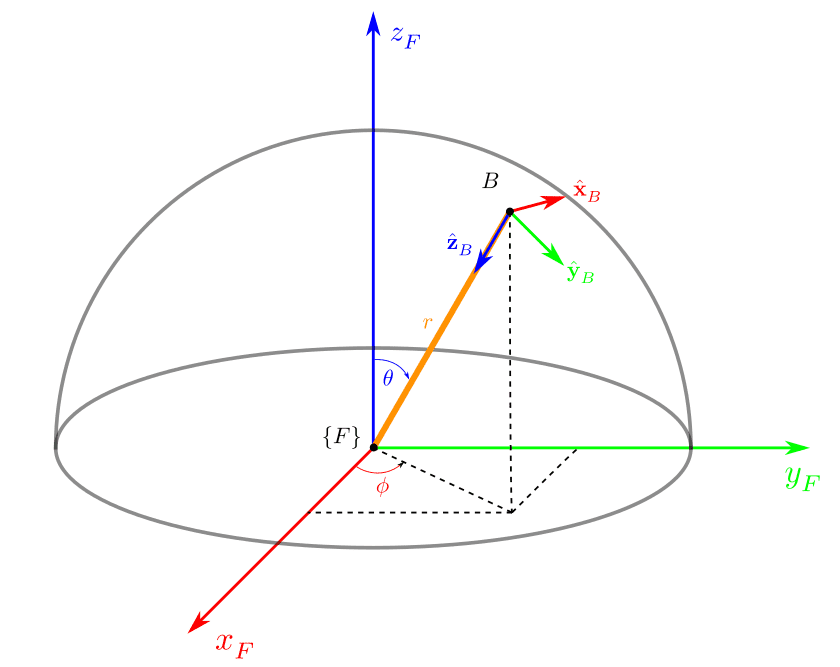
\includegraphics[width=12cm]{images/fulcrum-space.png}\\
\caption{Tool pose at target point $B$ calculated with respect to Fulcrum's reference frame $\lbrace F \rbrace$}
\end{figure}
\end{center}

The laparoscopic tool pose is given by the position and orientation vectors at target point $B$ with respect to the coordinate frame $\lbrace F \rbrace$.
The pose is given by the following transformation matrix
\[
{}^{F}T_B = \begin{bmatrix}
{}^{F}R_B & {}^{F}\mathbf{p}^{}_B \\
\mathbf{0} & 1 \\
\end{bmatrix}
\;\; where \;\;
{}^{F}R_B = \begin{bmatrix}
\hat{\mathbf{x}}^{}_B & \hat{\mathbf{y}}^{}_B & \hat{\mathbf{z}}^{}_B \\
\end{bmatrix}
\]

\begin{equation}
\hat{\mathbf{x}}^{}_B = \hat{\mathbf{θ}} = cos(θ)cos(φ)\hat{\mathbf{x}}^{}_F + cos(θ)sin(φ)\hat{\mathbf{y}}^{}_F - sin(θ)\hat{\mathbf{z}}^{}_F
= \begin{bmatrix}
cos(θ)cos(φ) \\
cos(θ)sin(φ) \\
- sin(θ) \\
\end{bmatrix}
\end{equation}

\begin{equation}
\hat{\mathbf{y}}^{}_B = \hat{\mathbf{φ}} = -sin(φ)\hat{\mathbf{x}}^{}_F + cos(φ)\hat{\mathbf{y}}^{}_F
= \begin{bmatrix}
-sin(φ) \\
cos(φ) \\
0 \\
\end{bmatrix}
\end{equation}

\begin{equation}
\hat{\mathbf{z}}^{}_B = - \hat{\mathbf{r}} = - (sin(θ)cos(φ)\hat{\mathbf{x}}^{}_F + sin(θ)sin(φ)\hat{\mathbf{y}}^{}_F + cos(θ)\hat{\mathbf{z}}^{}_F)
= \begin{bmatrix}
-sin(θ)cos(φ) \\
-sin(θ)sin(φ) \\
-cos(θ) \\
\end{bmatrix}
\end{equation}

The position of the point $B$ is given in spherical coordinates by:
\begin{itemize}
	\item $r=ρ$ : outside penetration of laparoscopic tool
	\item $θ=β$ : altitude angle
	\item $φ=α$ : orientation angle
\end{itemize}
thus the position with respect to the coordinate frame $\lbrace F \rbrace$ is given by
\begin{equation}
{}^{F}\mathbf{p}^{}_B = \begin{bmatrix}
ρsin(β)cos(α) \\
ρsin(β)sin(α) \\
ρcos(β) \\
\end{bmatrix} = ρ \hat{\mathbf{r}}
\end{equation}

The above goal point must be the same as the $TCP$ point of the robot's end-effector. This means, that this pose must be converted with respect to the robot's reference frames.
\[
{}^{U}T^{}_{TCP} = {}^{U}T^{}_{B}
\]
\[
{}^{U}T^{}_{0} \; {}^{0}T^{}_{7} \; {}^{7}T^{}_{TCP} = {}^{U}T^{}_{F} \; {}^{F}T^{}_{B}
\]
\begin{equation}
{}^{0}T^{}_{7} = {}^{U}T^{-1}_{0} \; {}^{U}T^{}_{F} \; {}^{F}T^{}_{B} \; {}^{7}T^{-1}_{TCP}
\end{equation}


\subsection{Trajectory planning in cartesian coordinates}
\label{subsection:pivot-motions}

On this section, some basic pivoting trajectories around the fulcrum point, are presented. In all of the following three example pivoting motions, we have made 
the assumption that the position and orientation of the ${F}$ reference frame is precisely known, which is however not applicable in real-life scenarios ()

\subsubsection{Circular trajectory of tool tip}

\begin{center}
\begin{figure}[H]
\centering
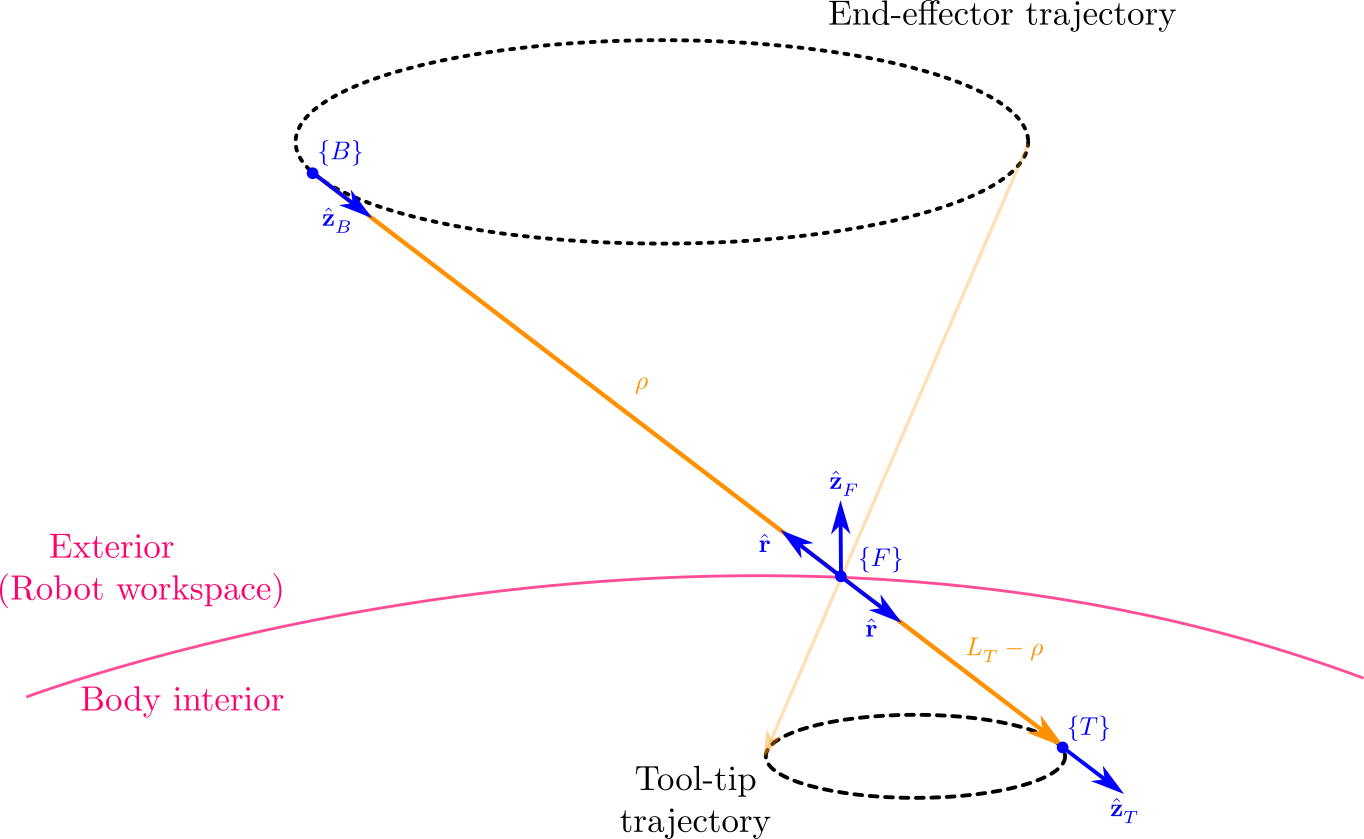
\includegraphics[width=12cm]{images/circular-trajectory-wrt-fulcrum.png}\\
\caption{Circular trajectory of tool tip with respect to Fulcrum reference frame}
\end{figure}
\end{center}

To generate a circular trajectory for the pivot movement we must specify the center of the circle 
and a vector whose magnitude is the radius of the circle and it’s direction gives the orientation 
of the plane that the circle lies at. The simplest case of a circular trajectory is the one, 
whose circle lies in a plane parallel to the xy plane.


We first consider the motion of the laparoscopic tool tip on a circle parallel to a z-plane, with respect to the $\lbrace F \rbrace$ coordinate frame.
\begin{equation}
(x^{}_{F} - x^{}_{F0})^2 + (y^{}_{F} - y^{}_{F0})^2 = r_0^2, \;\; z^{}_{F} = z^{}_{F0}
\end{equation}
It's often more convenient to express trajectories in a parametric form, which makes it easier to calculate all the waypoints of the trajectory
\begin{equation}
\begin{cases}
x^{}_{F} = r_0cos(2πs) + x^{}_{F0} \\
y^{}_{F} = r_0sin(2πs) + y^{}_{F0} \\
z^{}_{F} = z^{}_{F0}
\end{cases} ,
\;\;
s \in [0, 1]
\end{equation}

After having calculated the cartesian coordinates we can calculate the spherical coordinates as follows

\begin{equation}
\label{eqns:cartesian-to-spherical}
\begin{cases}
r = \sqrt{x^{2}_{F} + y^{2}_{F} + z^{2}_{F}} \\
θ = atan2 \left( \sqrt{x^{2}_{F} + y^{2}_{F}}, z^{}_{F} \right) \\
φ = atan2(y^{}_{F}, x^{}_{F})
\end{cases}
\end{equation}

\subsubsection{Circular arc trajectory of tool tip}

To generate a circular arc trajectory for a pivot motion we must specify the same parameters as 
in the circular trajectory as well as the length of the arc or the total angle of the arc 
section.


\subsubsection{Line segment trajectory of tool tip}

\begin{center}
\begin{figure}[H]
\centering
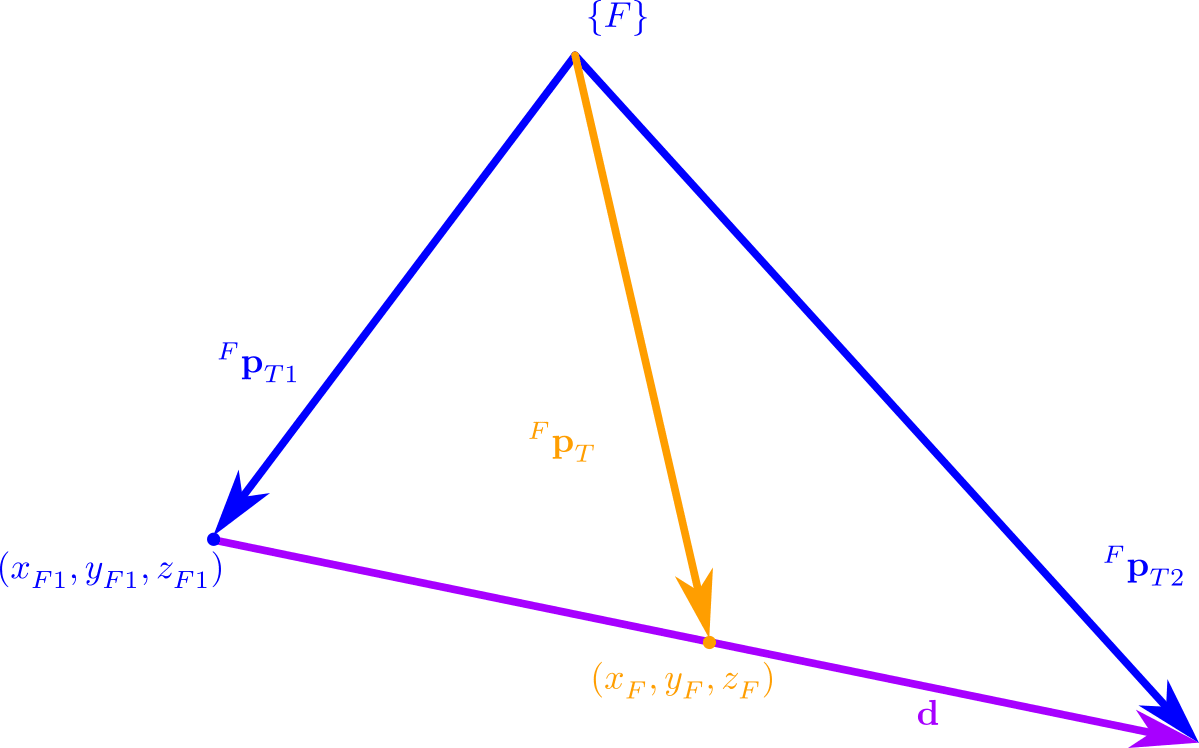
\includegraphics[width=10cm]{images/line-segment-trajectory-wrt-fulcrum.png}\\
\caption{Line segment trajectory of tool tip with respect to Fulcrum reference frame}
\end{figure}
\end{center}
\[
\mathbf{d} = {}^{F}\mathbf{p}^{}_{T2} - {}^{F}\mathbf{p}^{}_{T1} = [l, m, n]^\top
\]
\[
{}^{F}\mathbf{p}^{}_{T} = [x^{}_{F}, y^{}_{F}, z^{}_{F}]^\top
\]
\[
{}^{F}\mathbf{p}^{}_{T} = {}^{F}\mathbf{p}^{}_{T1} + s\mathbf{d}
\]
\[
s = \frac{x^{}_{F} - x^{}_{F1}}{l} = \frac{y^{}_{F} - y^{}_{F1}}{m} = \frac{z^{}_{F} - z^{}_{F1}}{n} \;\; s \in [0, 1]
\]

\begin{equation}
\begin{cases}
x^{}_{F} = sl + x^{}_{F1} = (1-s)x^{}_{F1} + sx^{}_{F2} \\
y^{}_{F} = sm + y^{}_{F1} = (1-s)y^{}_{F1} + sy^{}_{F2} \\
z^{}_{F} = sn + z^{}_{F1} = (1-s)z^{}_{F1} + sz^{}_{F2}
\end{cases}
\end{equation}

After having calculated the cartesian coordinates we can calculate the spherical coordinates using the \ref{eqns:cartesian-to-spherical} equations.

The line segment trajectory of tool tip, as analysed in this section needs no implementation as 
it is already implemented in the ROS MoveIt library and can be used by calling the method 
\textbf{computeCartesianPath}.

\subsubsection{Cubic Spline trajectory of tool tip}

A useful mathematical tool to construct a smooth curve that visits every point from a given set of waypoints are \textbf{cubic splines}. A cubic spline is 
constructed using smaller curves that are described by a polynomial of 3rd order. Let $\left\lbrace \mathbf{P}_0, \mathbf{P}_1, \ldots , \mathbf{P}_n \right\rbrace$ 
be a set of waypoints, where each point has coordinates $\mathbf{P}_i = [x_i, y_i, z_i]^\top$. Then between each 2 points a cubic 
polynomial can be constructed (one for each coordinate, 3 in total). The following equations are for the $x$-coordinate and in the exact same way one can 
calculate the cubic polynomials for the $y,z$ coordinates as well. For each pair of waypoints we want to calculate the following cubic polynomial
\begin{equation}
\label{cubic-polynomial}
x_i(s) = a_i(s-s_i)^3 + b_i(s-s_i)^2 + c_i(s-s_i) + d_i, \hspace{3em} s_i \leqslant s \leqslant s_{i+1}
\end{equation}

The polynomial in equation \ref{cubic-polynomial} has four unknowns which means that four additional equations are needed to get a unique solution and fully 
define the polynomial. These equations can be formed using the boundary conditions for the first and last point of each curve.
\begin{equation}
x_i(s_i) = x_i
\end{equation}
\begin{equation}
x_i(s_{i+1}) = x_{i+1}
\end{equation}
\begin{equation}
\dot{x}_i(s_i) = \dot{x}_i
\end{equation}
\begin{equation}
\dot{x}_i(s_{i+1}) = \dot{x}_{i+1}
\end{equation}

First we solve for $c_i$ and $d_i$, which can easily be calculated as follows
\begin{equation}
\label{di-eq}
d_i = x_i(s_i) = x_i
\end{equation}
and by taking the derivative of \ref{cubic-polynomial}, we can calculate $c_i$
\begin{equation}
\label{cubic-polynomial-first-derivative}
\dot{x}_i(s_i) = 3a_i(s-s_i)^2 + 2b_i(s-s_i) + c_i
\end{equation}
\begin{equation}
\label{ci-eq}
c_i = \dot{x}_i(s_i) = \dot{x}_i
\end{equation}

By substituting $s = s_{i+1}$ in \ref{cubic-polynomial} and \ref{cubic-polynomial-first-derivative}, by using equations \ref{ci-eq}, \ref{di-eq} and if 
we set $σ = s_{i+1}-s_i$ for brevity, we get the following two equations
\begin{equation}
\label{xi1}
x_{i+1} = x_i(s_{i+1}) = a_i σ^3 + b_i σ^2 + c_i σ + x_i
\end{equation}
and
\begin{equation}
\label{xdi1}
\dot{x}_{i+1} = \dot{x}_i(s_{i+1}) = 3a_i σ^2 + 2b_i σ + \dot{x}_i
\end{equation}

By multiplying \ref{xdi1} by $σ$ and \ref{xi1} by $-3$ and add them together we get
\[
\dot{x}_{i+1}σ - 3x_{i+1} = -b_iσ^2 -2\dot{x}_iσ - 3x_i
\]
\begin{equation}
b_i = \frac{1}{σ^2} (3x_{i+1} -3x_i - \dot{x}_{i+1}σ - 2\dot{x}_iσ)
\end{equation}

Similarly, by multiplying \ref{xdi1} by $σ$ and \ref{xi1} by $-2$ and add them together we get
\[
\dot{x}_{i+1}σ - 2x_{i+1} = a_iσ^3 -\dot{x}_iσ - 2x_i
\]
\begin{equation}
a_i = \frac{1}{σ^3} (\dot{x}_{i+1}σ - 2x_{i+1} + \dot{x}_iσ +2x_i)
\end{equation}

\begin{center}
\begin{figure}[H]
\centering
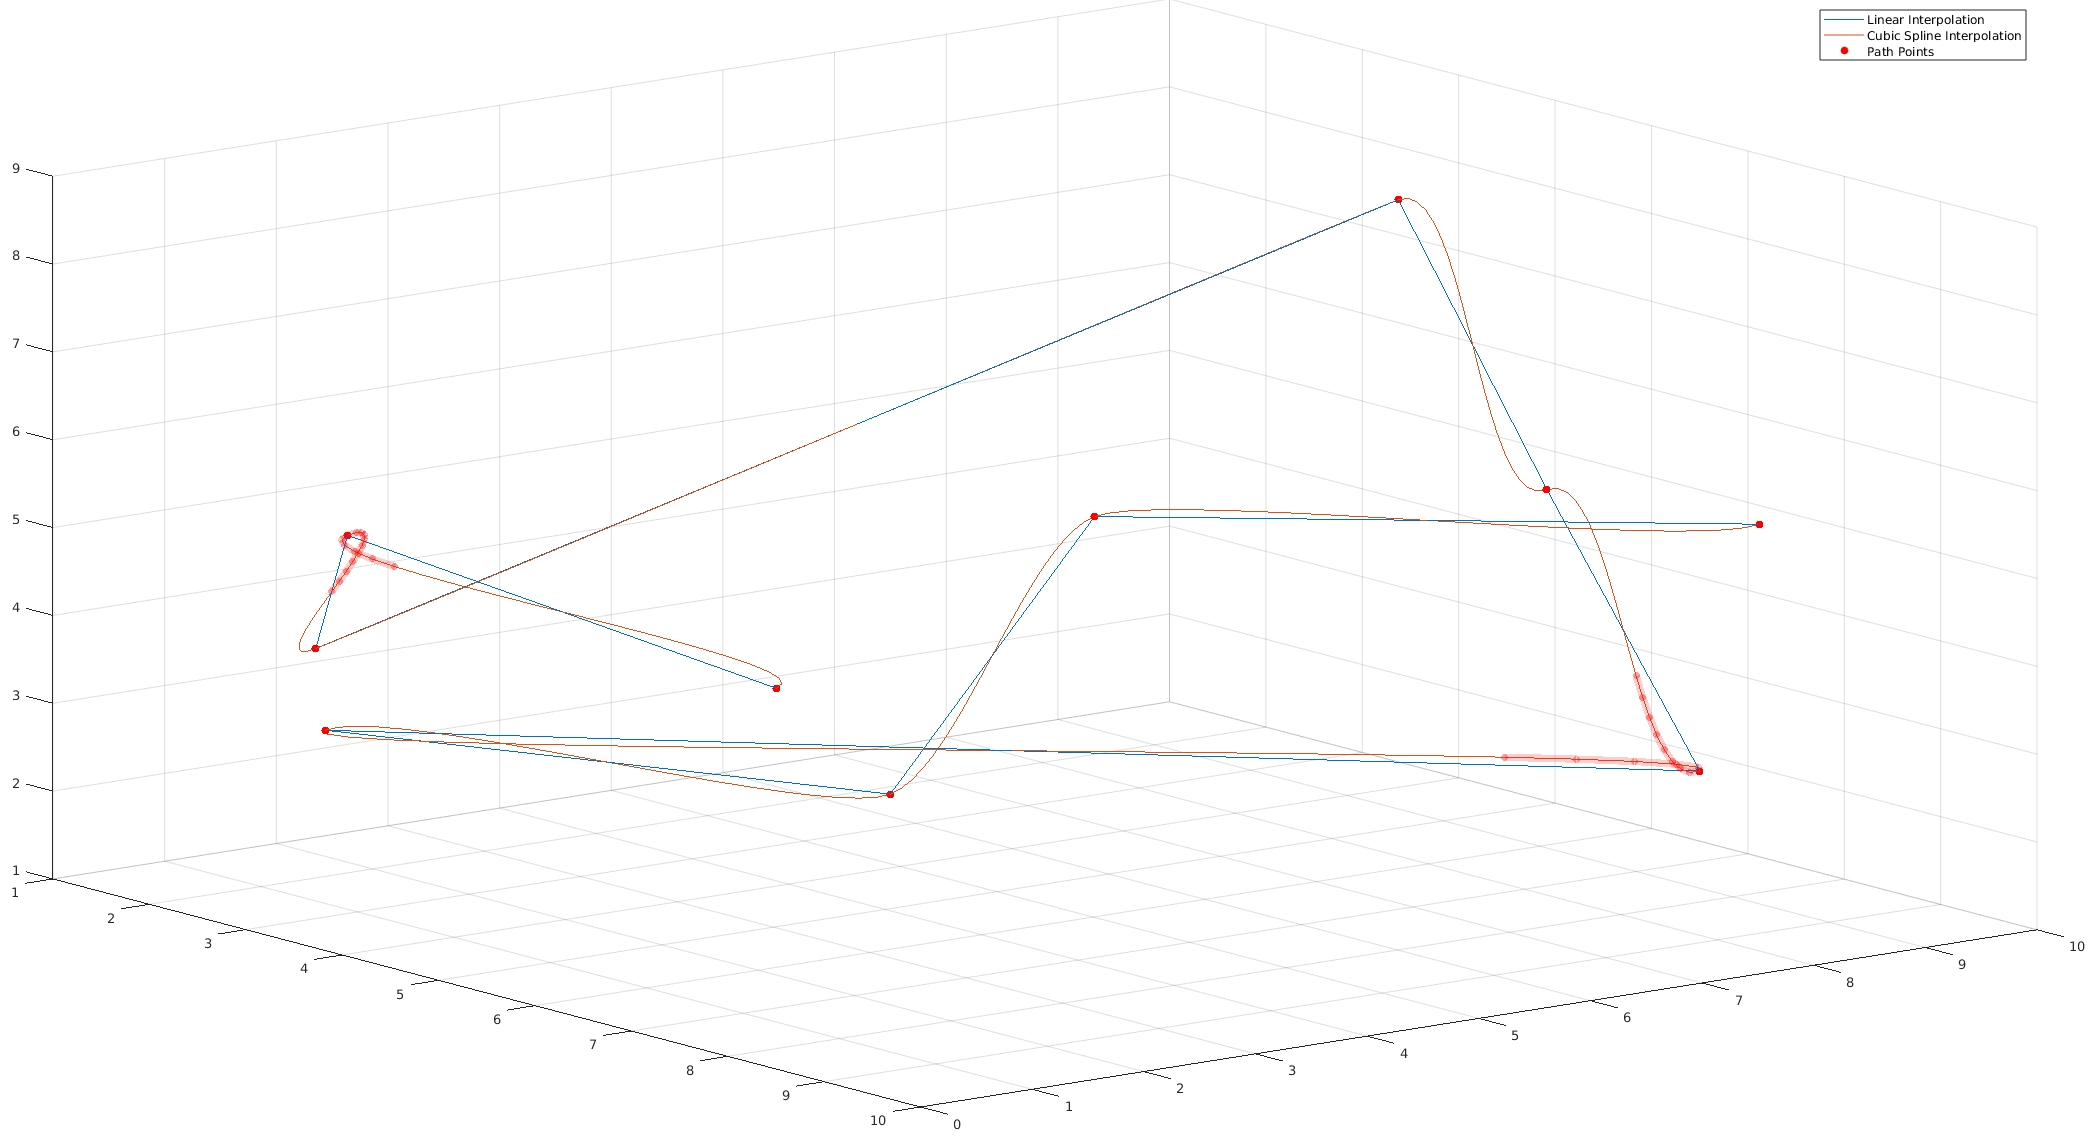
\includegraphics[width=\textwidth]{images/cubic-spline-path1.png}\\
\caption{Cubic Spline curve with 10 waypoints} 
\label{b-spline-explanation}
\end{figure}
\end{center}


\subsubsection{B-Spline trajectory of tool tip}

The \textbf{B-Splines} are smooth curves which are constructed from \textbf{B\'ezier} curves. A B\'ezier curve is a parametric smooth curve and is a $k$-th order interpolation of $k+1$ control points.

\begin{center}
\begin{figure}[H]
\centering
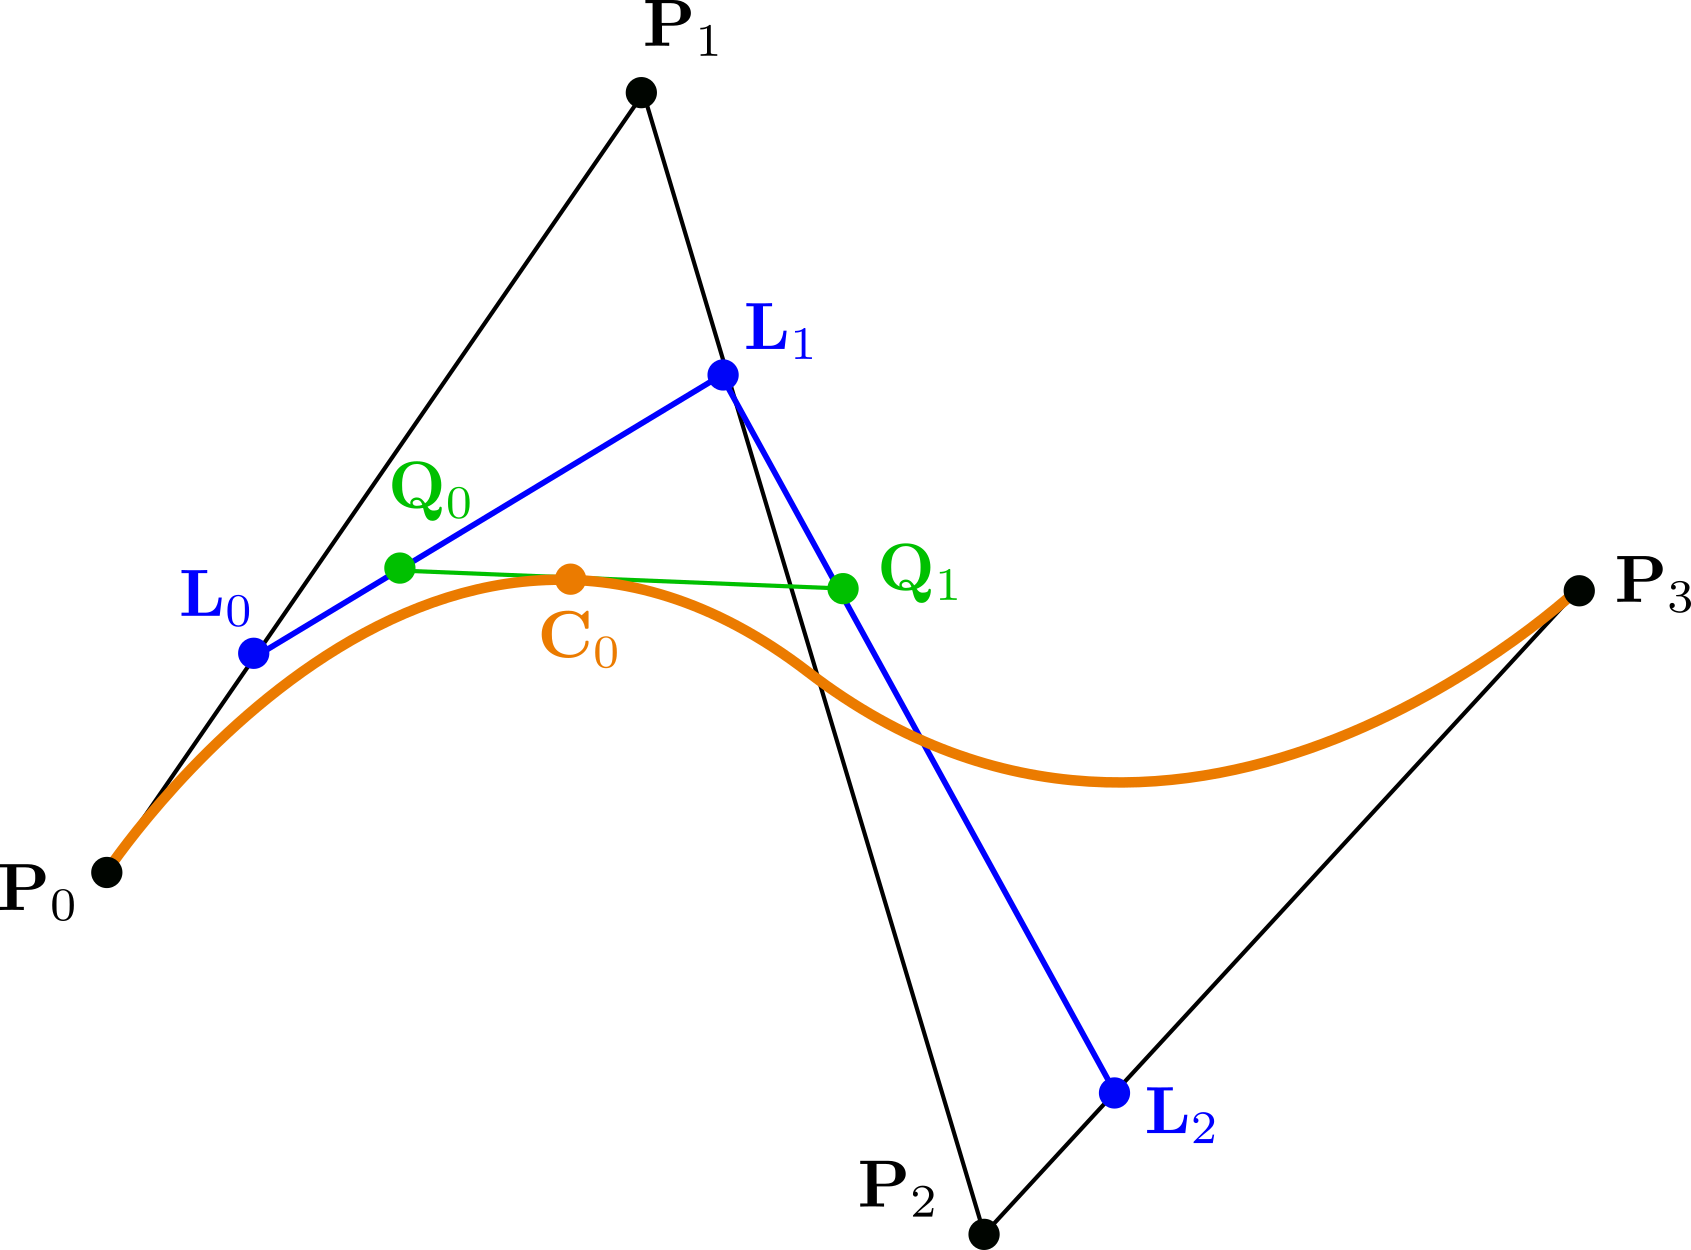
\includegraphics[width=0.5\textwidth]{images/bezier-curve.png}\\
\caption{Cubic B\'ezier curve calculated using cubic interpolation of 4 control points} 
\end{figure}
\end{center}

We first calculate the linear interpolation of the control points
\begin{equation}
\mathbf{L}_0(s) = (1-s)\mathbf{P}_0 + s\mathbf{P}_1
\end{equation}
\[
\mathbf{L}_1(s) = (1-s)\mathbf{P}_1 + s\mathbf{P}_2
\]
\[
\mathbf{L}_2(s) = (1-s)\mathbf{P}_2 + s\mathbf{P}_3
\]
The next step is to calculate the quadratic interpolation of the control points or equivalently, the linear interpolation of the previously calculated points $\mathbf{L}_0,\mathbf{L}_1,\mathbf{L}_2$
\[
\mathbf{Q}_0(s) = (1-s)\mathbf{L}_0(s) + s\mathbf{L}_1(s)
\]
\begin{equation}
\mathbf{Q}_0(s) = (1-s)^2\mathbf{P}_0 + 2(1-s)s\mathbf{P}_1 + s^2\mathbf{P}_2
\end{equation}
\[
\mathbf{Q}_1(s) = (1-s)^2\mathbf{P}_1 + 2(1-s)s\mathbf{P}_2 + s^2\mathbf{P}_3
\]
Similarly for the last step, we calculate the cubic interpolation of the control points or equivalently, the linear interpolation of the previously calculated points $\mathbf{Q}_0,\mathbf{Q}_1$
\[
\mathbf{C}_0(s) = (1-s)\mathbf{Q}_0(s) + s\mathbf{Q}_1(s)
\]
\begin{equation}
\mathbf{C}_0(s) = (1-s)^3\mathbf{P}_0 +3(1-s)^2 s\mathbf{P}_1 + 3(1-s)s^2\mathbf{P}_2 + s^3\mathbf{P}_3
\end{equation}

The cubic B\'ezier curve can also be calculated using the following more compact equation, in matrix form
\begin{equation}
\mathbf{C}_0(t) = \begin{bmatrix} \mathbf{P}_0 & \mathbf{P}_1 & \mathbf{P}_2 & \mathbf{P}_3 \end{bmatrix} 
\begin{bmatrix} 
-1 & 3 & -3 & 1 \\
3 & -6 & 3 & 0 \\
-3 & 3 & 0 & 0 \\
1 & 0 & 0 & 0
\end{bmatrix}
\begin{bmatrix}
s^3 \\ s^2 \\ s \\ 1
\end{bmatrix}
\end{equation}

A $k$-degree \textbf{B-Spline} curve defined by $n+1$ control points will consist of $n-k+1$ B\'ezier curves. For example if we want to construct a cubic B-Spline using 6 control points, then we will need to construct 
and connect together 3 B\'ezier curves.

\begin{center}
\begin{figure}[H]
\centering
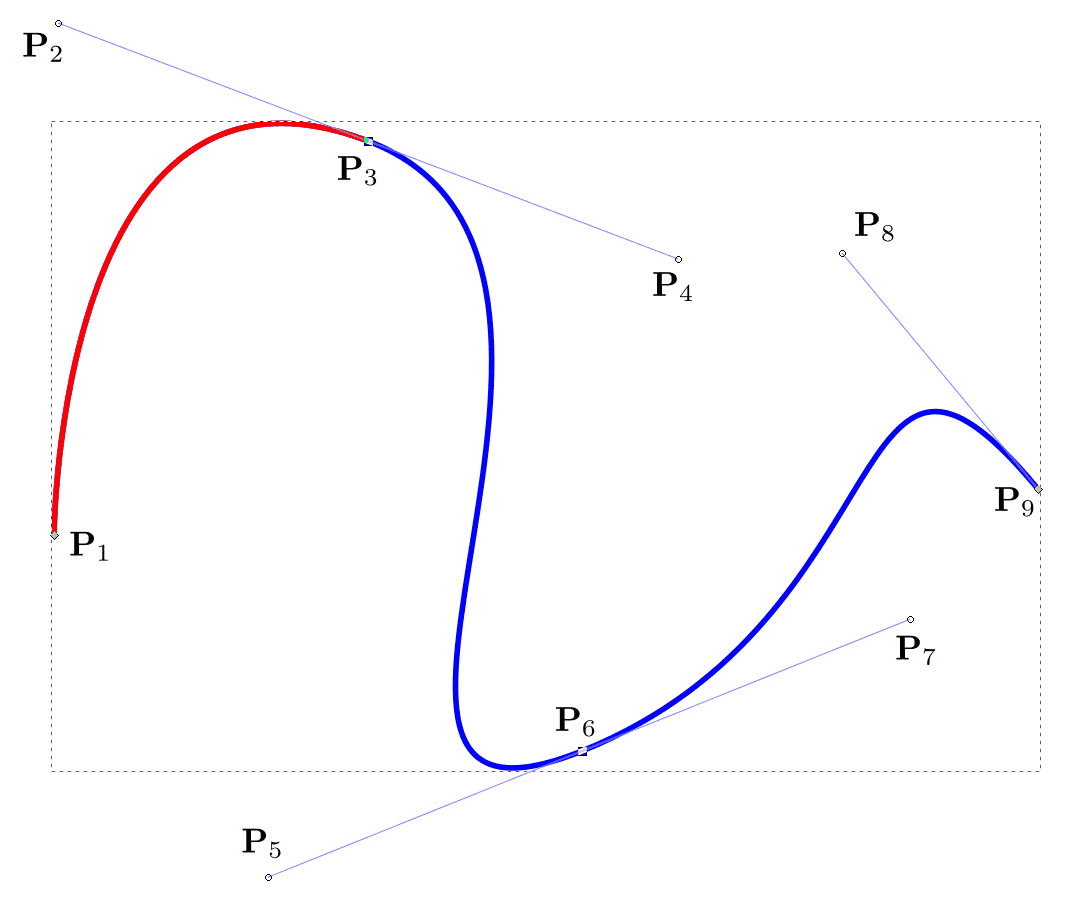
\includegraphics[width=0.6\textwidth]{images/b-spline-explanation.png}\\
\caption{B-Spline curve constructed from 3 B\'ezier curves. The first B\'ezier curve colored in red is a quadratic one and the following two are both cubic.} 
\label{b-spline-explanation}
\end{figure}
\end{center}

In most cases the B-Spline curves are constructed by starting from a quadratic B\'ezier curve, which is constructed from 3 control points and then all other 
parts of the curve are constructed from cubic B\'ezier curves, each constructed from 4 control points. As shown in figure \ref{b-spline-explanation}, the B-Spline 
curves do not pass from all control points. This means that if we have a path formed by a set of waypoints and we want the robot to pass from all of them, then 
in order to construct a B-Spline trajectory we will need additional intermediary points. The first and last points are part of the curve and the other control 
points are not. If no additional points can be calculated then the robot will not pass from all the points, which in some cases is also acceptable and useful.

\begin{center}
\begin{figure}[H]
\centering
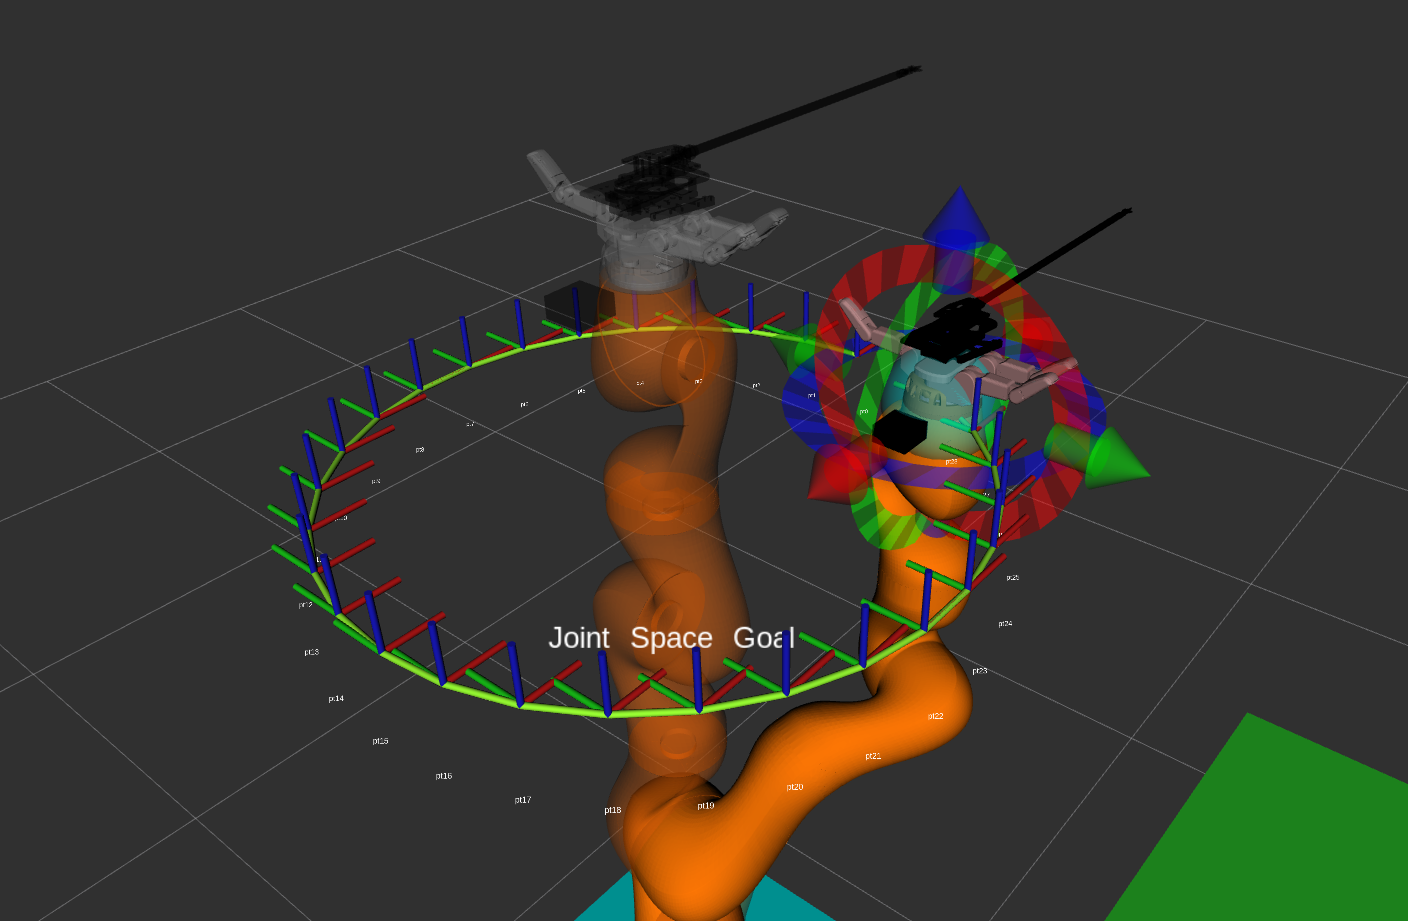
\includegraphics[width=0.7\textwidth]{images/simple_circular_traj1.png}\\
\caption{Circlular trajectory around the z axis of the home position of the robot}
\label{fig:circ-traj-out-of-angle-range}
\end{figure}
\end{center}

It is very important that the designed trajectory respects the joints angles' range. For example
depending on the starting position of the circular trajectory depicted at figure 
\ref{fig:circ-traj-out-of-angle-range}, the robot arm may reach it's joint bounds and in order to 
continue executing the trajectory it will have to make a sudden jump to reset the angles. 
This could have serious side-effects for both the surgical task and thus the patient, as well as 
for the operating staff, who control the robot.


\subsection{Trajectory planning in joint angles space}

\begin{center}
\begin{figure}[H]
\centering
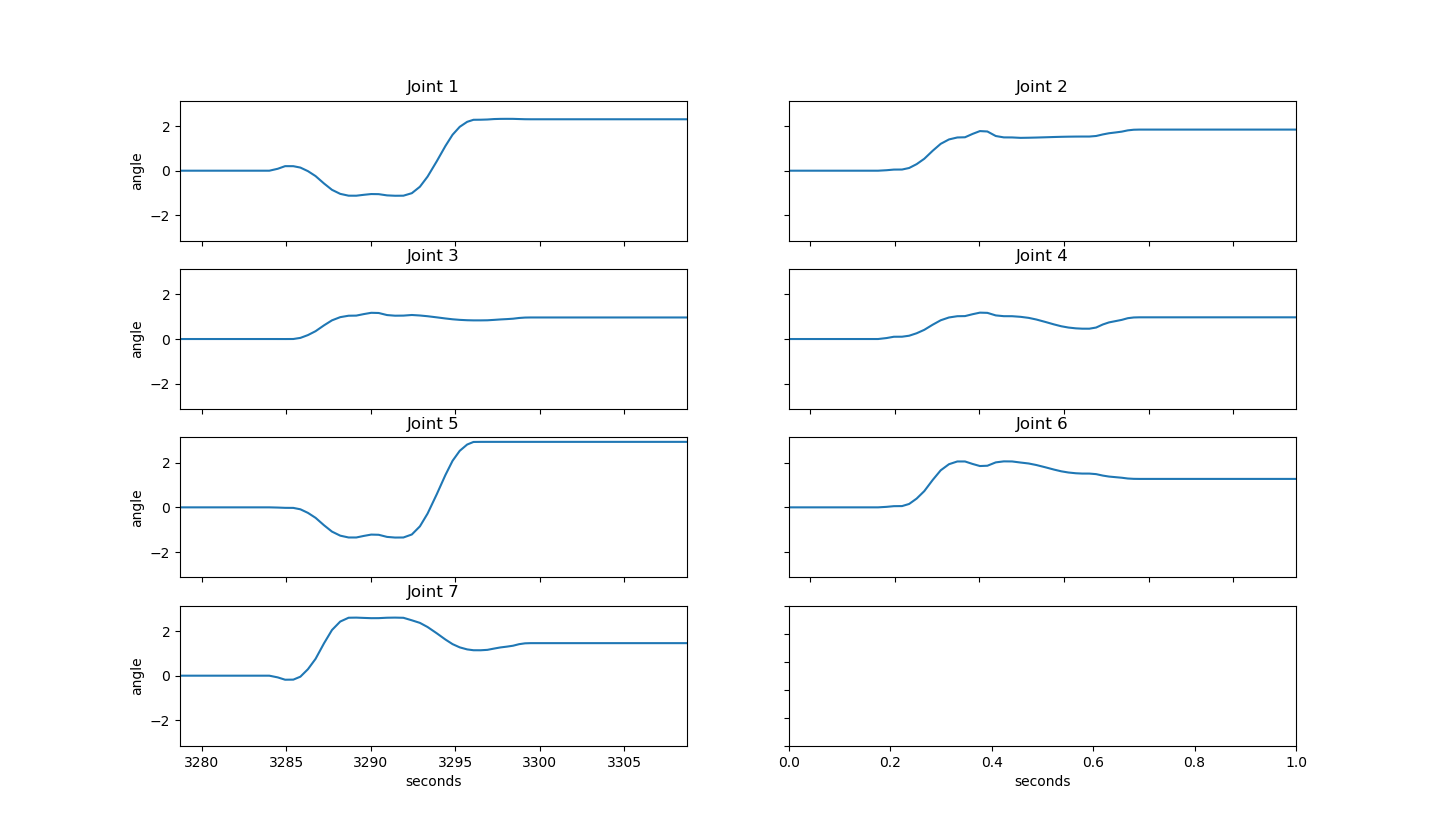
\includegraphics[width=\textwidth]{images/trajectory1-test1.png}\\
\caption{Trajectory diagrams in joints space.}
\end{figure}
\end{center}


\subsubsection{Polynomials of 5th order}


\subsubsection{Trapezoidal velocity profile}


\subsubsection{S-Curve velocity profile}

%\newpage
\section{ROS framework}

\subsection{Introduction to the ROS framework}

\textbf{ROS} is an open-source robotics software framework. It is a meta-operating system, which means that it provides its own 
abstractions on top of the host's operating system including filesystem, hardware abstractions, low-level device control, 
package management and networking. It also provides tools and services to develop large, scalable 
robotics software, it supports a wide variety of libraries and programming languages and it has a huge community, support and 
documentation resources.


\begin{enumerate}
\item \textbf{ROS Filesystem}
\begin{itemize}
\item \textbf{Packages}
\item \textbf{Metapackages}
\item \textbf{Package Manifests}
\item \textbf{Messages}
\item \textbf{Services}
\item \textbf{Launch files}
\end{itemize}

\item \textbf{ROS Computation Graph}
\begin{itemize}
\item \textbf{Nodes}
\item \textbf{Master}
\item \textbf{Parameter Server}
\item \textbf{Topics}
\item \textbf{Bags}
\end{itemize}

\item \textbf{ROS Community}
\begin{itemize}
\item \textbf{Distributions}
\item \textbf{Repositories}
\item \textbf{ROS Wiki}
\item \textbf{ROS Answers}
\end{itemize}

\item \textbf{ROS Tools}
\begin{itemize}
\item \textbf{Gazebo}
\item \textbf{RViz}
\item \textbf{Moveit}
\item \textbf{Filesystem tools}
\end{itemize}
\end{enumerate}

\begin{center}
\begin{figure}[H]
\centering
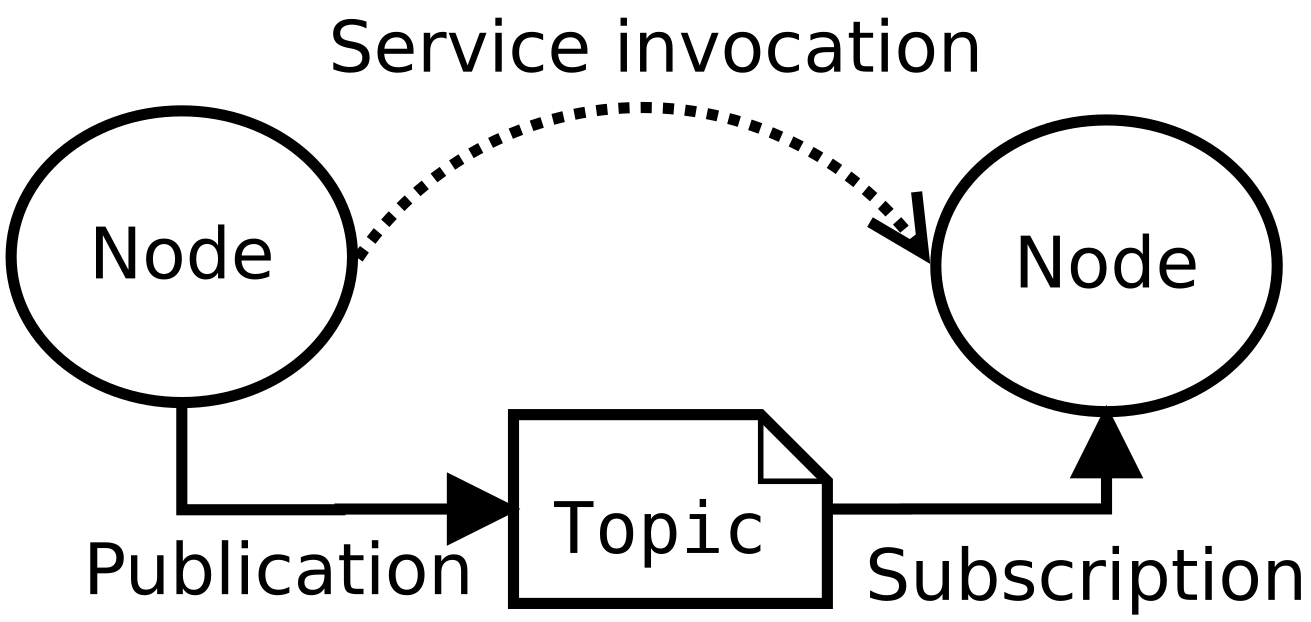
\includegraphics{images/ROS_basic_concepts_topics_nodes.png}\\
\caption{Communication diagram of 2 ROS nodes with a topic and a service}
\end{figure}
\end{center}


\subsection{Gazebo simulation environment}

\begin{center}
\begin{figure}[H]
\centering
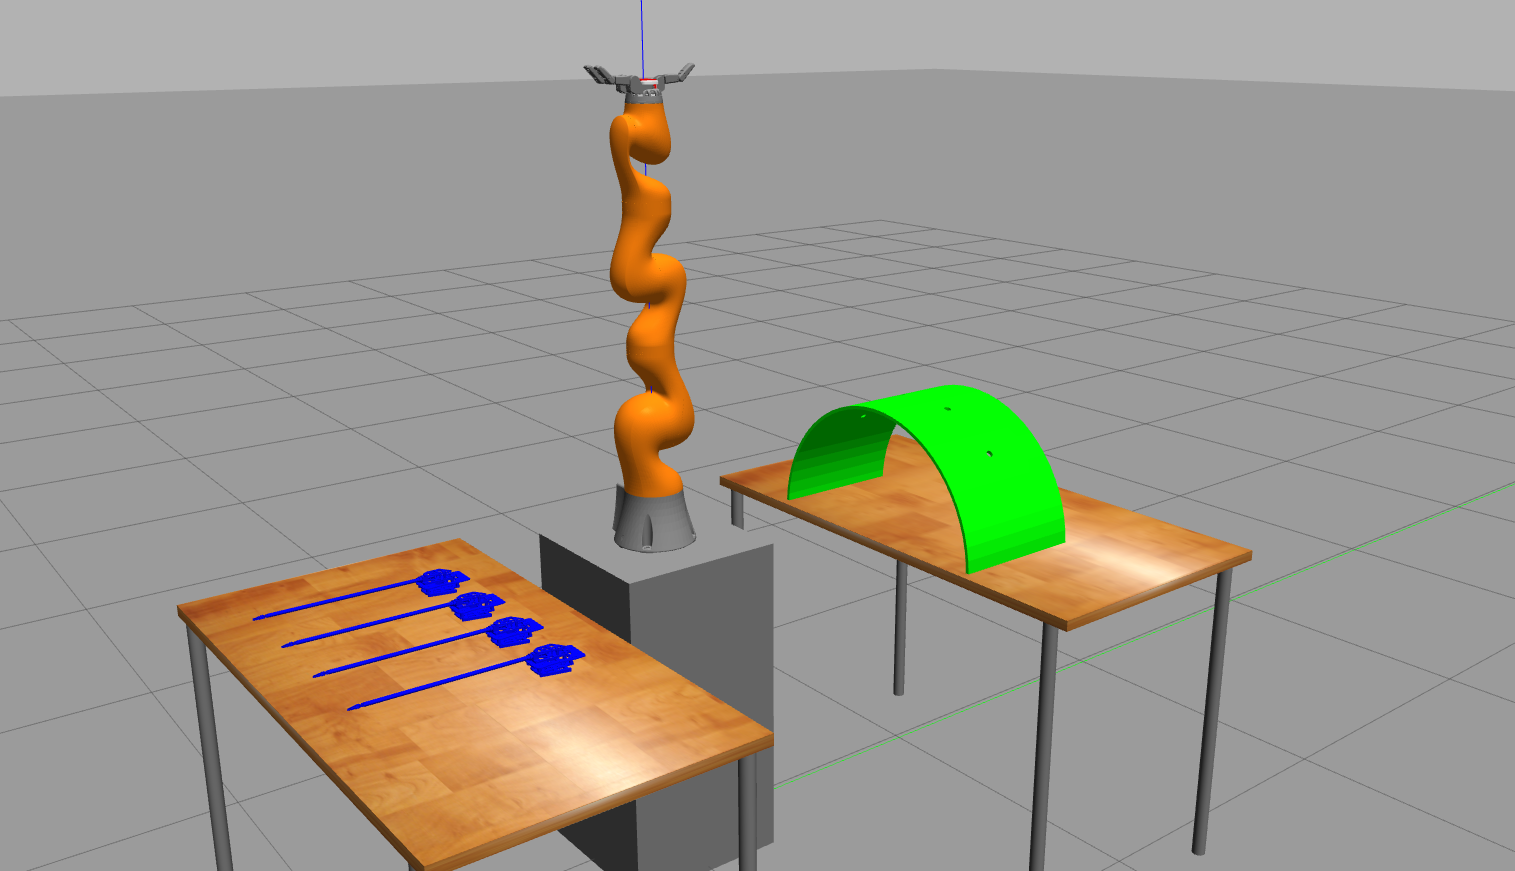
\includegraphics[width=12cm]{images/gazebo-sim1.png}\\
\caption{Simulation environment in Gazebo}
\end{figure}
\end{center}

The main environment setup of this thesis was designed using the Gazebo simulation environment and 
it consists of the following objects:
\begin{itemize}
\item the robot arm, KUKA\textsuperscript \textregistered iiwa14 lbr, being at the center of the setup
\item the robot base, so that the robot arm can better reach the tools and the surgical site and have more flexibility in movement
\item 2 tables, one for the tools and one for the surgical site
\item 4 surgical tools, using a modified version of the surgical tools used in the Raven II surgical platform
\item a mounting dock, which has holes that have the same role as the trocars (small tubes from 
which the surgical tool is inserted). Initially a mounting dock with 4 same holes of 4mm diameter was used, but it was later replaced with a new one with holes of variable diameters to test feasibility of pivot motions. Larger diameters means more space for motion planner to search for solution and thus more probable to find a solution.
\end{itemize}

\begin{center}
\begin{figure}[H]
\centering
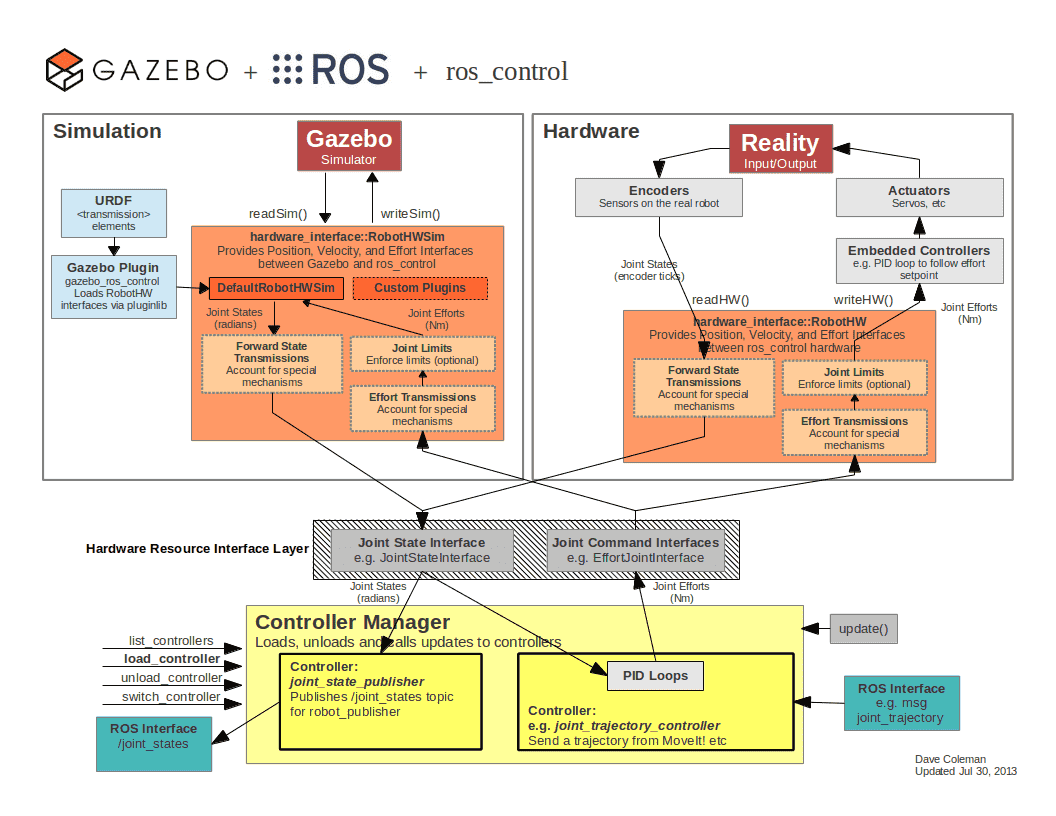
\includegraphics[width=12cm]{images/Gazebo_ros_transmission.png}\\
\caption{Control \& Hardware Interfaces in Gazebo and ROS}
\end{figure}
\end{center}


\subsection{Visualization with RViz}

RViz is one of the most important and most used tools in robotic applications development and is a 3D visualizer for the Robot Operating System framework. RViz functionality should not be confused 
with that of Gazebo, because the first one visualizes the robot state and the \textbf{perceived} world (perceived objects or other calculations related to the world) whereas the second one simulates the real world.

\begin{center}
\begin{figure}[H]
\centering
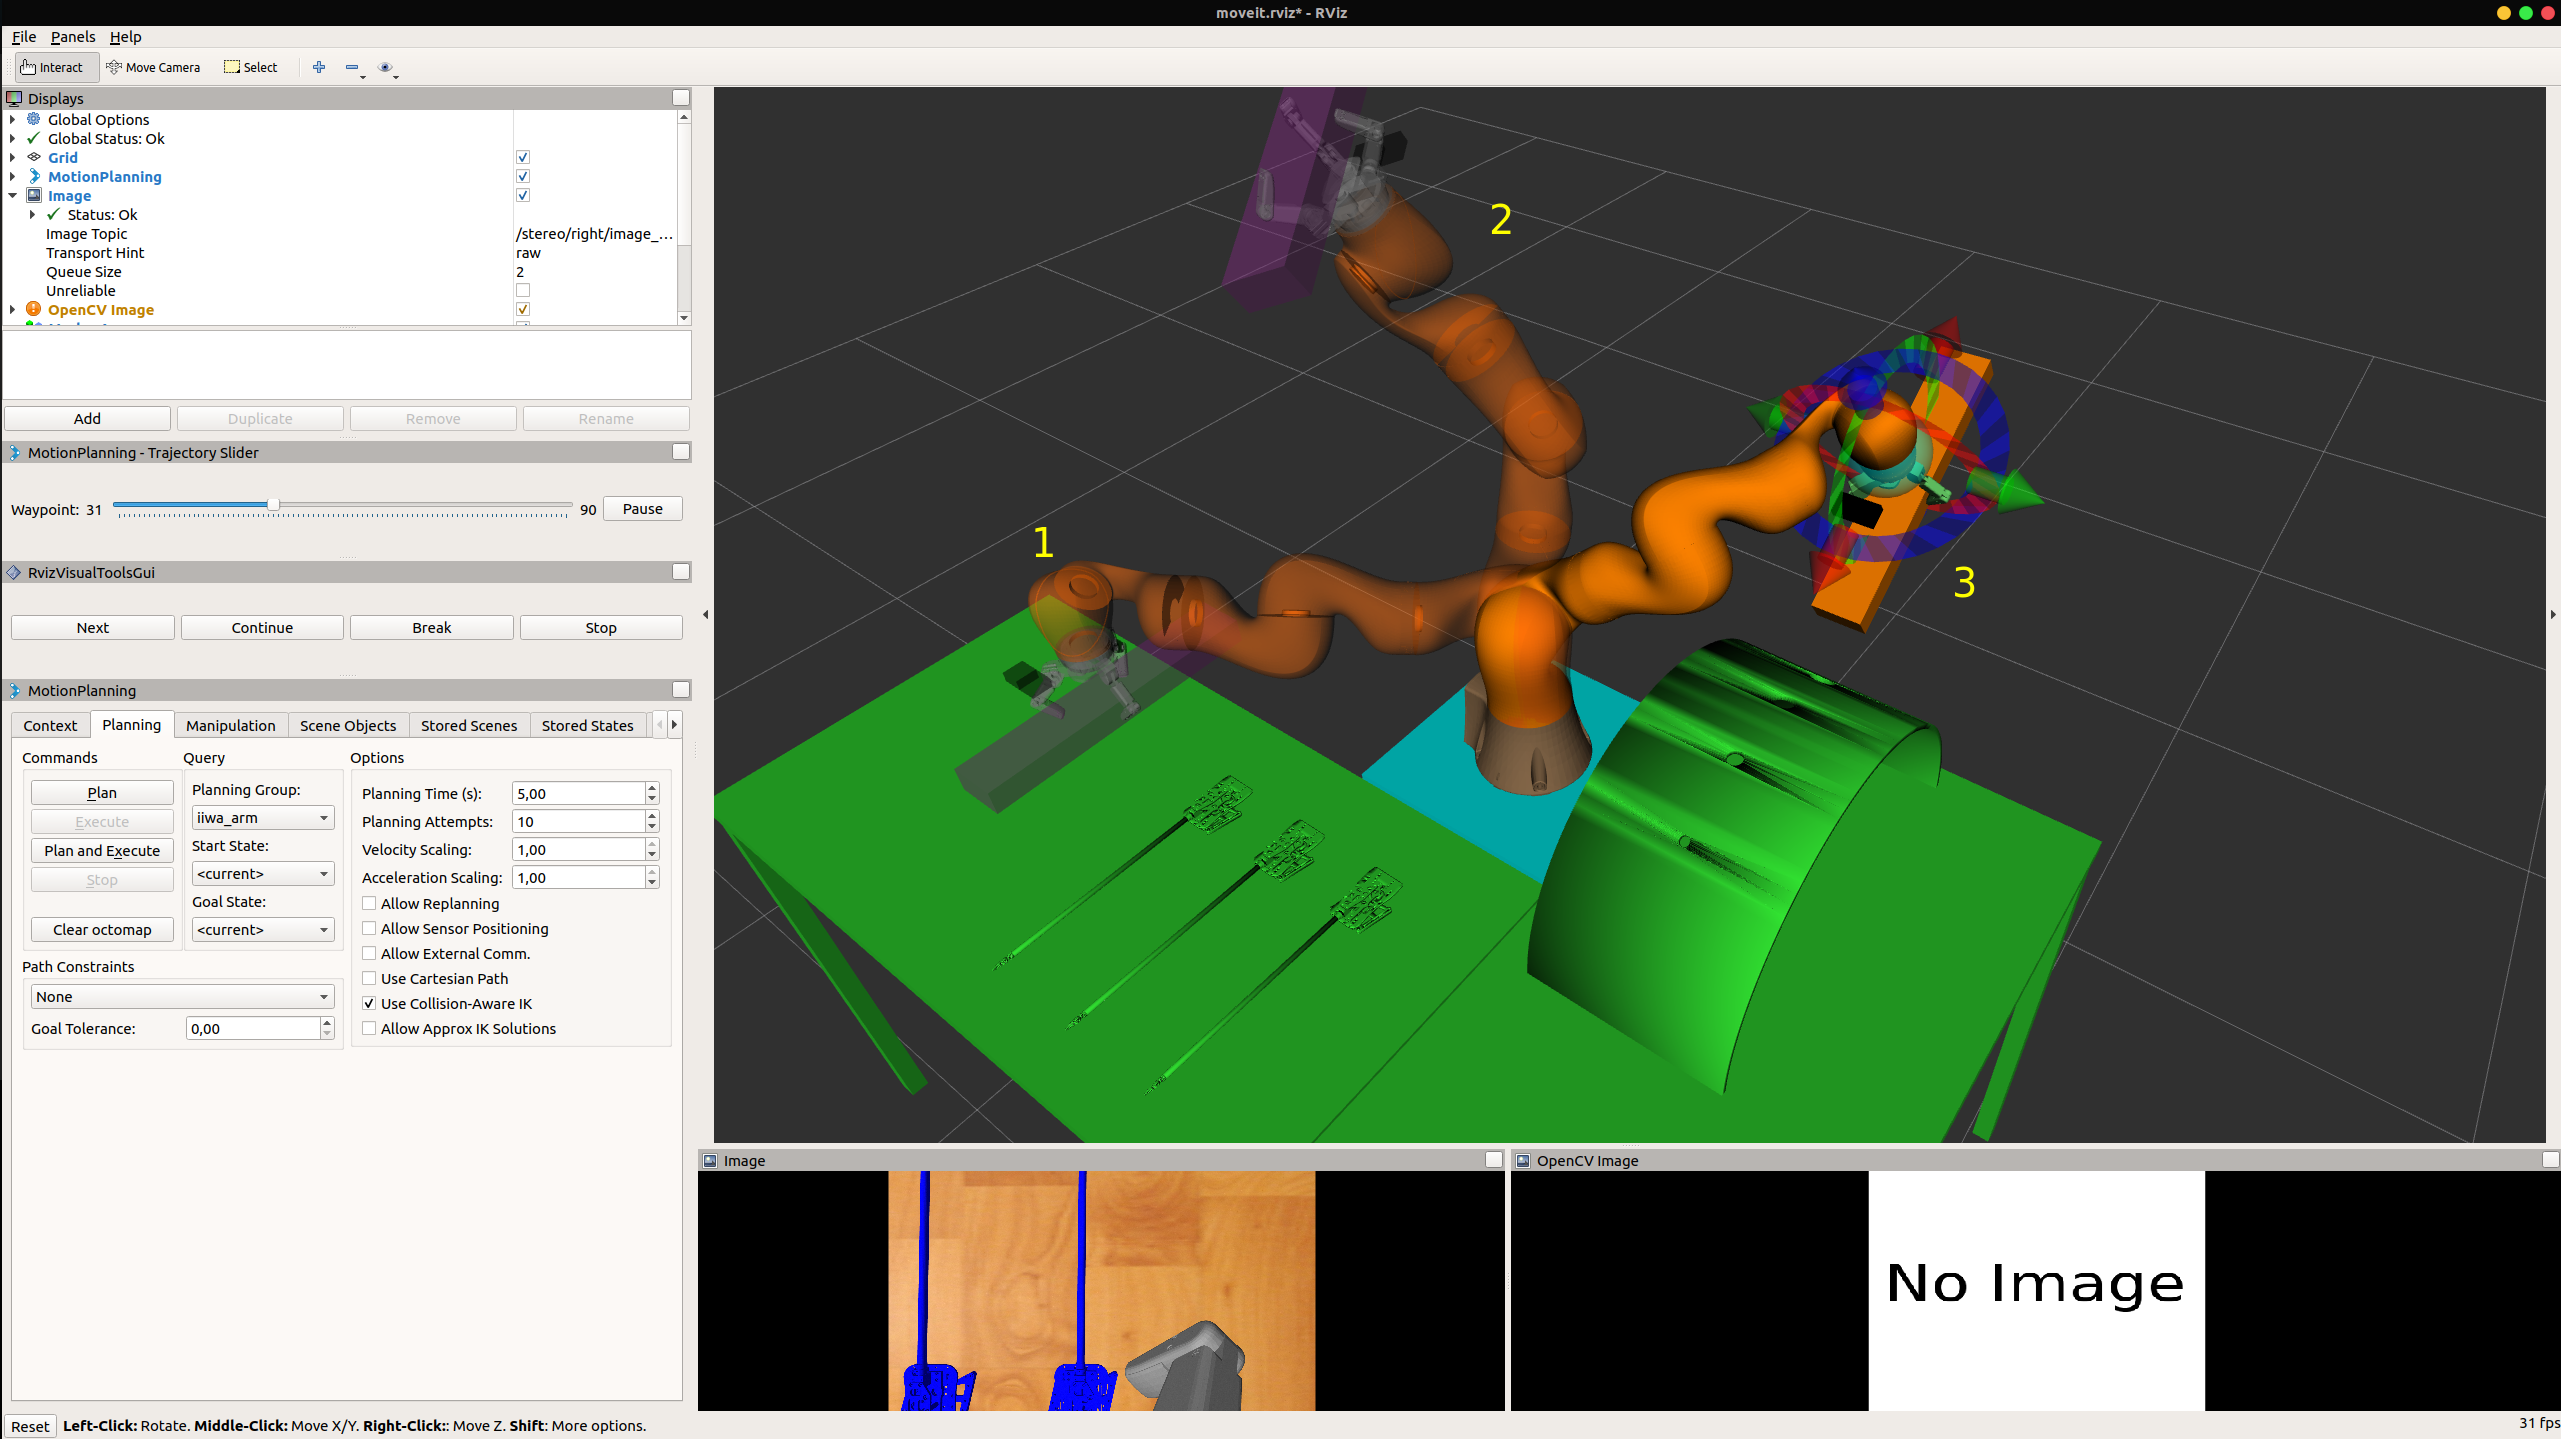
\includegraphics[width=\textwidth]{images/rviz.png}\\
\caption{RViz: Visualizing the robot state as well as the state of the perceived world\\
In this screenshot, various poses of the robot are shown: 1) the current actual real pose of the robot, 2) the planned pose and 3) the goal pose, which can 
freely be moved within the RViz environment}
\end{figure}
\end{center}

The objects that appear in RViz can either be visualized from approximations calculated from actual measurements from the robot (for example a point cloud) or can be manually loaded, in which case we make 
an assumption that the robot already "knows" the exact position, orientation, size and shape of the object, which is rarely the case in real life scenarios.
It is important to mention, that every such object is taken into consideration in collision checks and in path planning algorithms.

\subsection{Motion Planning with Moveit}

When using the Moveit ROS library a set of parameters need to be configured in order to generate the desired commands for the controller:
\begin{itemize}
	\item \textbf{Position tolerance}: The radius of the sphere that the end-effector must reach. This is the maximum allowed error in the target's position.
	This tolerance is typically much smaller inside the surgical site, to avoid fatalities.
	\item \textbf{Orientation tolerance}: The tolerance or maximum allowed error for roll, pitch and yaw, in radians
	\item \textbf{Maximum planning time}: Maximum amount of time to be used when planning a trajectory
	\item \textbf{Replanning}: Specify whether the robot is allowed to replan if it detects changes in the environment
	\item \textbf{Maximum planning attempts}: Number of times the motion plan is to be computed from scratch before the shortest solution is returned
	\item \textbf{Base frame}: The frame in respect to which the motion plan is calculated.
	\item \textbf{Jump threshold}: This parameter sets an upper bound to the amount of "jump" (change in distance) that can occur between two consecutive trajectory points in joint 
	positions. Disabling the jump threshold while operating real hardware can cause large unpredictable motions of redundant joints 
	and could be a safety issue
	\item \textbf{Velocity scaling factor}: The approaching motion needs to be slower. We reduce the speed of the robot arm via a scaling factor of the 
	maxiumum speed of each joint. Note this is not the speed of the end effector point
	\item \textbf{End-effector step}: The resolution at which the Cartesian path is interpolated or the max step in Cartesian translation
	\item \textbf{Planner algorithm}:
	\item \textbf{Fraction}: The fraction of the path achieved as described by the waypoints
\end{itemize}

Typical motion planning parameter values outside of surgical site:
\begin{itemize}
	\item Position tolerance: 50μm
	\item Orientation tolerance: 0.00005 deg
	\item Planning time: 10s
\end{itemize}

Typical motion planning parameter values inside surgical site:
\begin{itemize}
	\item Position tolerance:
	\item Orientation tolerance:
	\item Planning time
	\item End-effector interpolation step: 1mm
	\item Maximum velocity scaling factor
\end{itemize}

Sometimes the motion planner finds a solution but the execution from the controller is aborted. 
After many iterations of the same experiment this does not happen always, which means that the 
feasibility of the execution of the movement by the controller depends on the initial state of 
the robot, i.e. if initially some joints of the robot are at their boundaries, then the next 
commanded trajectory maybe unfeasible. Another reason that the path planner may fail is the 
probabilistic nature of the path planning algorithms (see also RRT and PRM algorithms in chapter 6).

At each time step it is important to publish a custom message containing all the information 
about the kinematic state of the robot. In this thesis a custom \textbf{ROS} message was created 
containing a tf transform with a 3D vector for the position and a quaternion for the rotation and 
a custom  6-by-7 matrix containing the values of the Jacobian. The MoveIt library, from which the 
kinematic state of the robot is obtained, returns the orientation of the end effector as a 3-by-3 
rotation matrix, but in the ROS tf message it must be expressed as a quaternion. To convert the 
matrix to a quaternion we first calculate the euler angles and then use these values to construct 
the quaternion “vector”. The quaternion representation of rotation is often preferred in robotic 
applications due to its efficiency in calculations and memory. To convert the transformation 
matrix to euler angles and then to quaternions the following formulas were used:
\[
T = 
\begin{bmatrix}
r_{11} & r_{12} & r_{13} & x \\
r_{21} & r_{22} & r_{23} & y \\
r_{31} & r_{32} & r_{33} & z \\
0 & 0 & 0 & 1\\
\end{bmatrix}
\]

\[
φ = atan2(r_{21}, r_{11})
\]

\[
θ = atan2(-r_{31}, \sqrt{r_{11}^2 + r_{21}^2})
\]

\[
ψ = atan2(r_{32}, r_{33})
\]

where $T$ is the transformation matrix and $φ, θ, ψ$ are the roll, pitch and yaw (Euler) angles.


%\newpage
\section{Experiments and Results}

\subsection{Experiments}

\subsubsection{Robot Planner 1}

In this first experiment we are testing some simple trajectories with the surgical tool already attached to the robot arm's end effector.
The path is designed using the appropriate coordinates and orientations so that the robot begins from the home position, then visits the table with the surgical 
tools and then visits the other table on top of which the mounting dock is placed. Upon arrival at the mounting dock, the robot inserts the tool inside a hole
(we consider these holes to be a simplistic alternative to the trocars used in real operations), then executes a simple pivot motion, while the tool is still 
inserted and then the tool gets ejected from the mounting dock's hole.\\

The aim of this experiment is to test the overall behaviour of the robot inside the work space, before implementing more complex path planning algorithms.

\begin{center}
\begin{figure}[H]
\centering
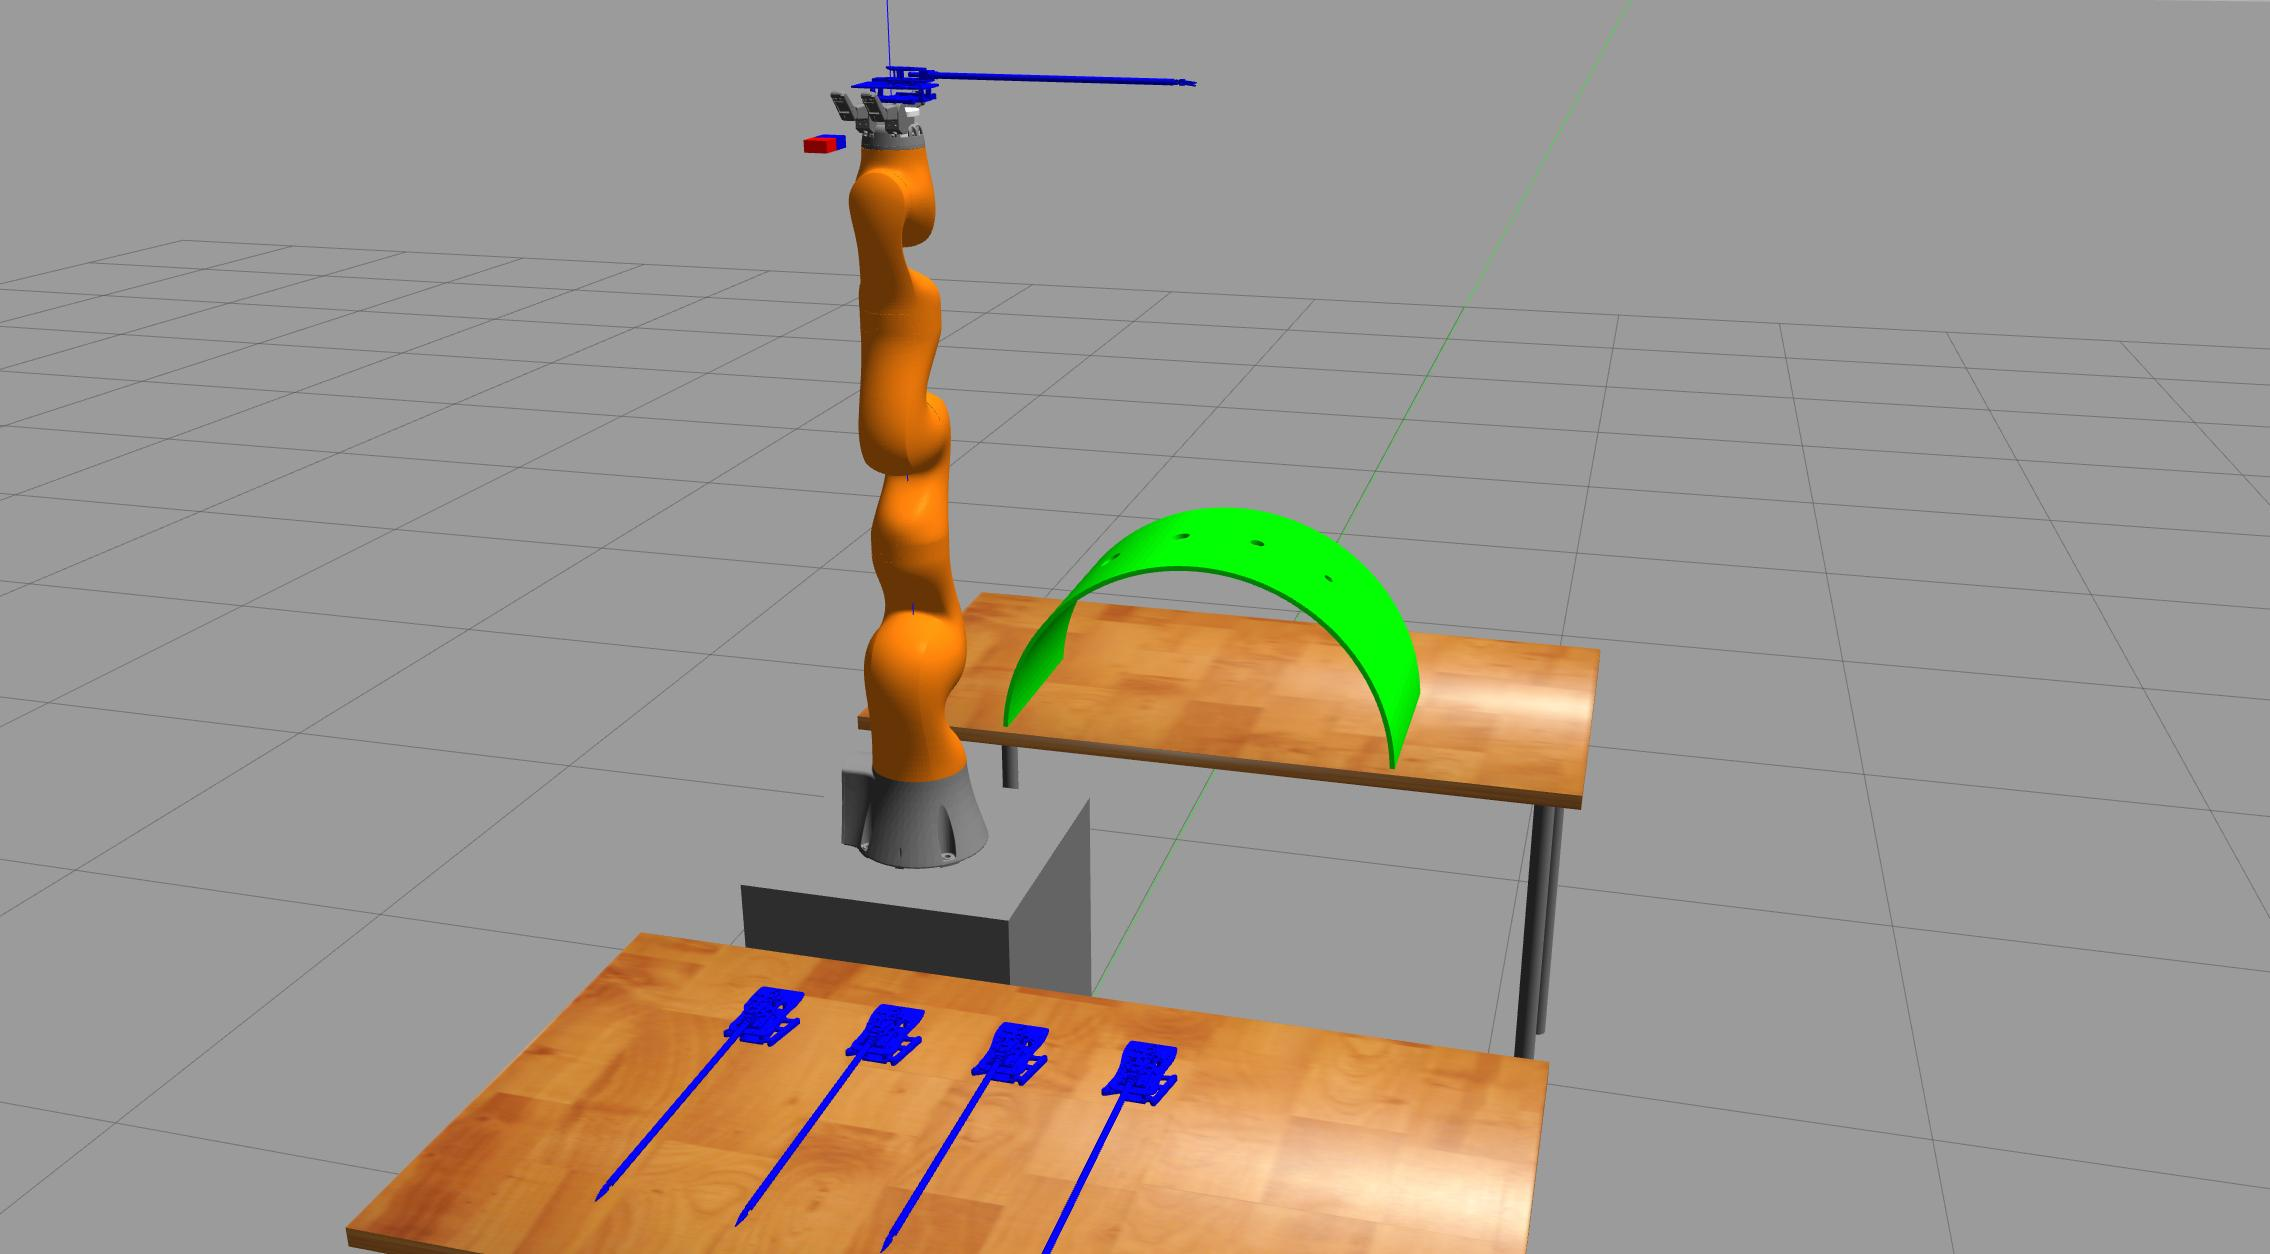
\includegraphics[width=0.3\textwidth]{images/robot_planner1/robot_planner1_1}
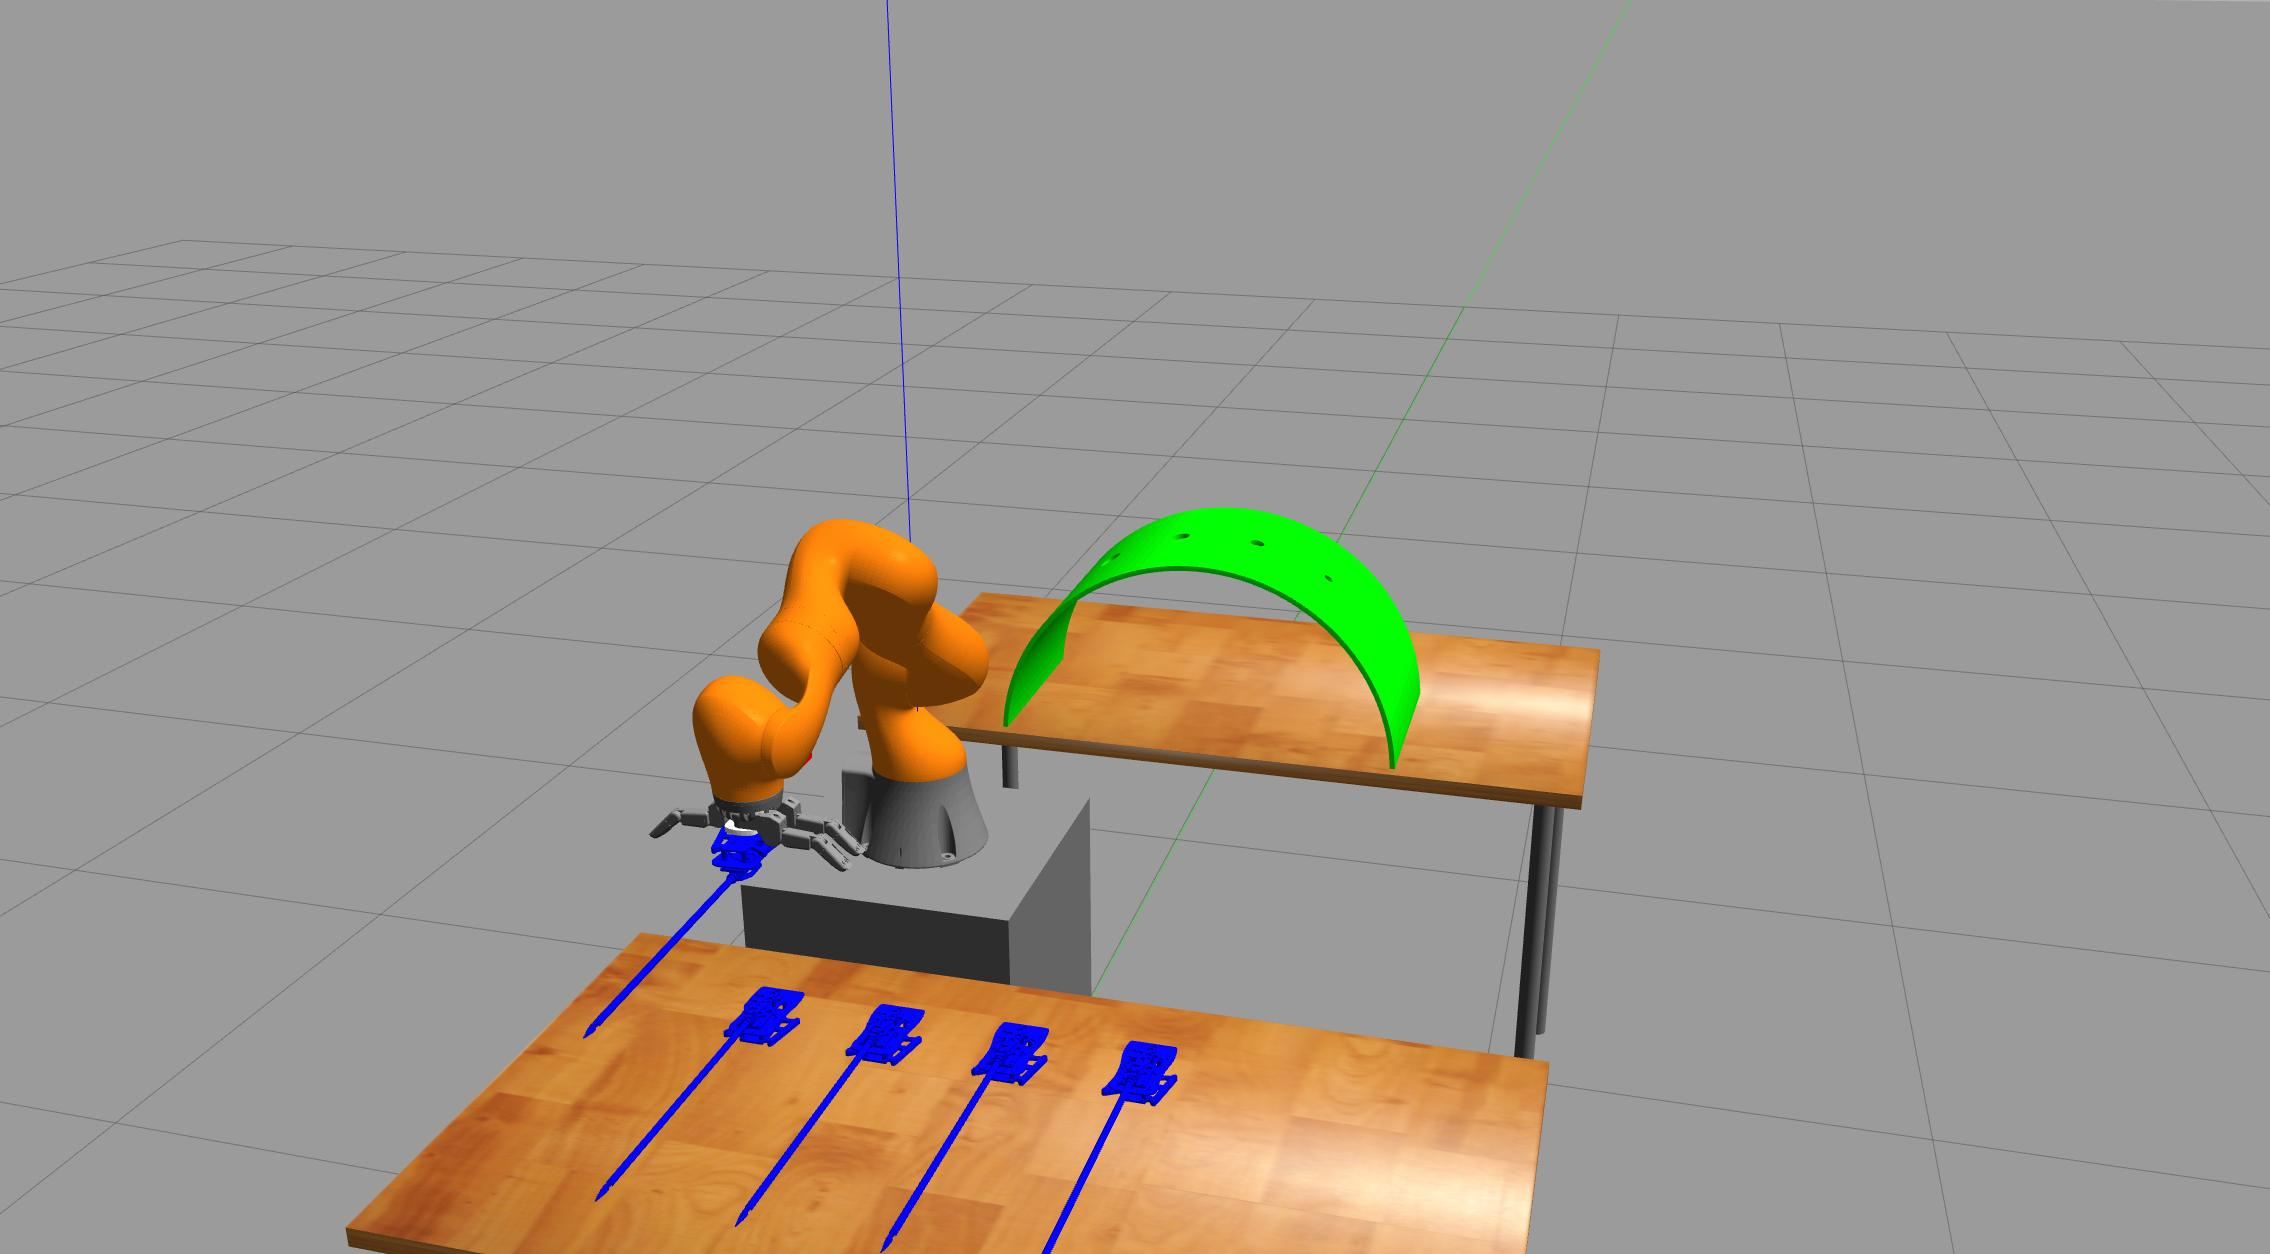
\includegraphics[width=0.3\textwidth]{images/robot_planner1/robot_planner1_2}
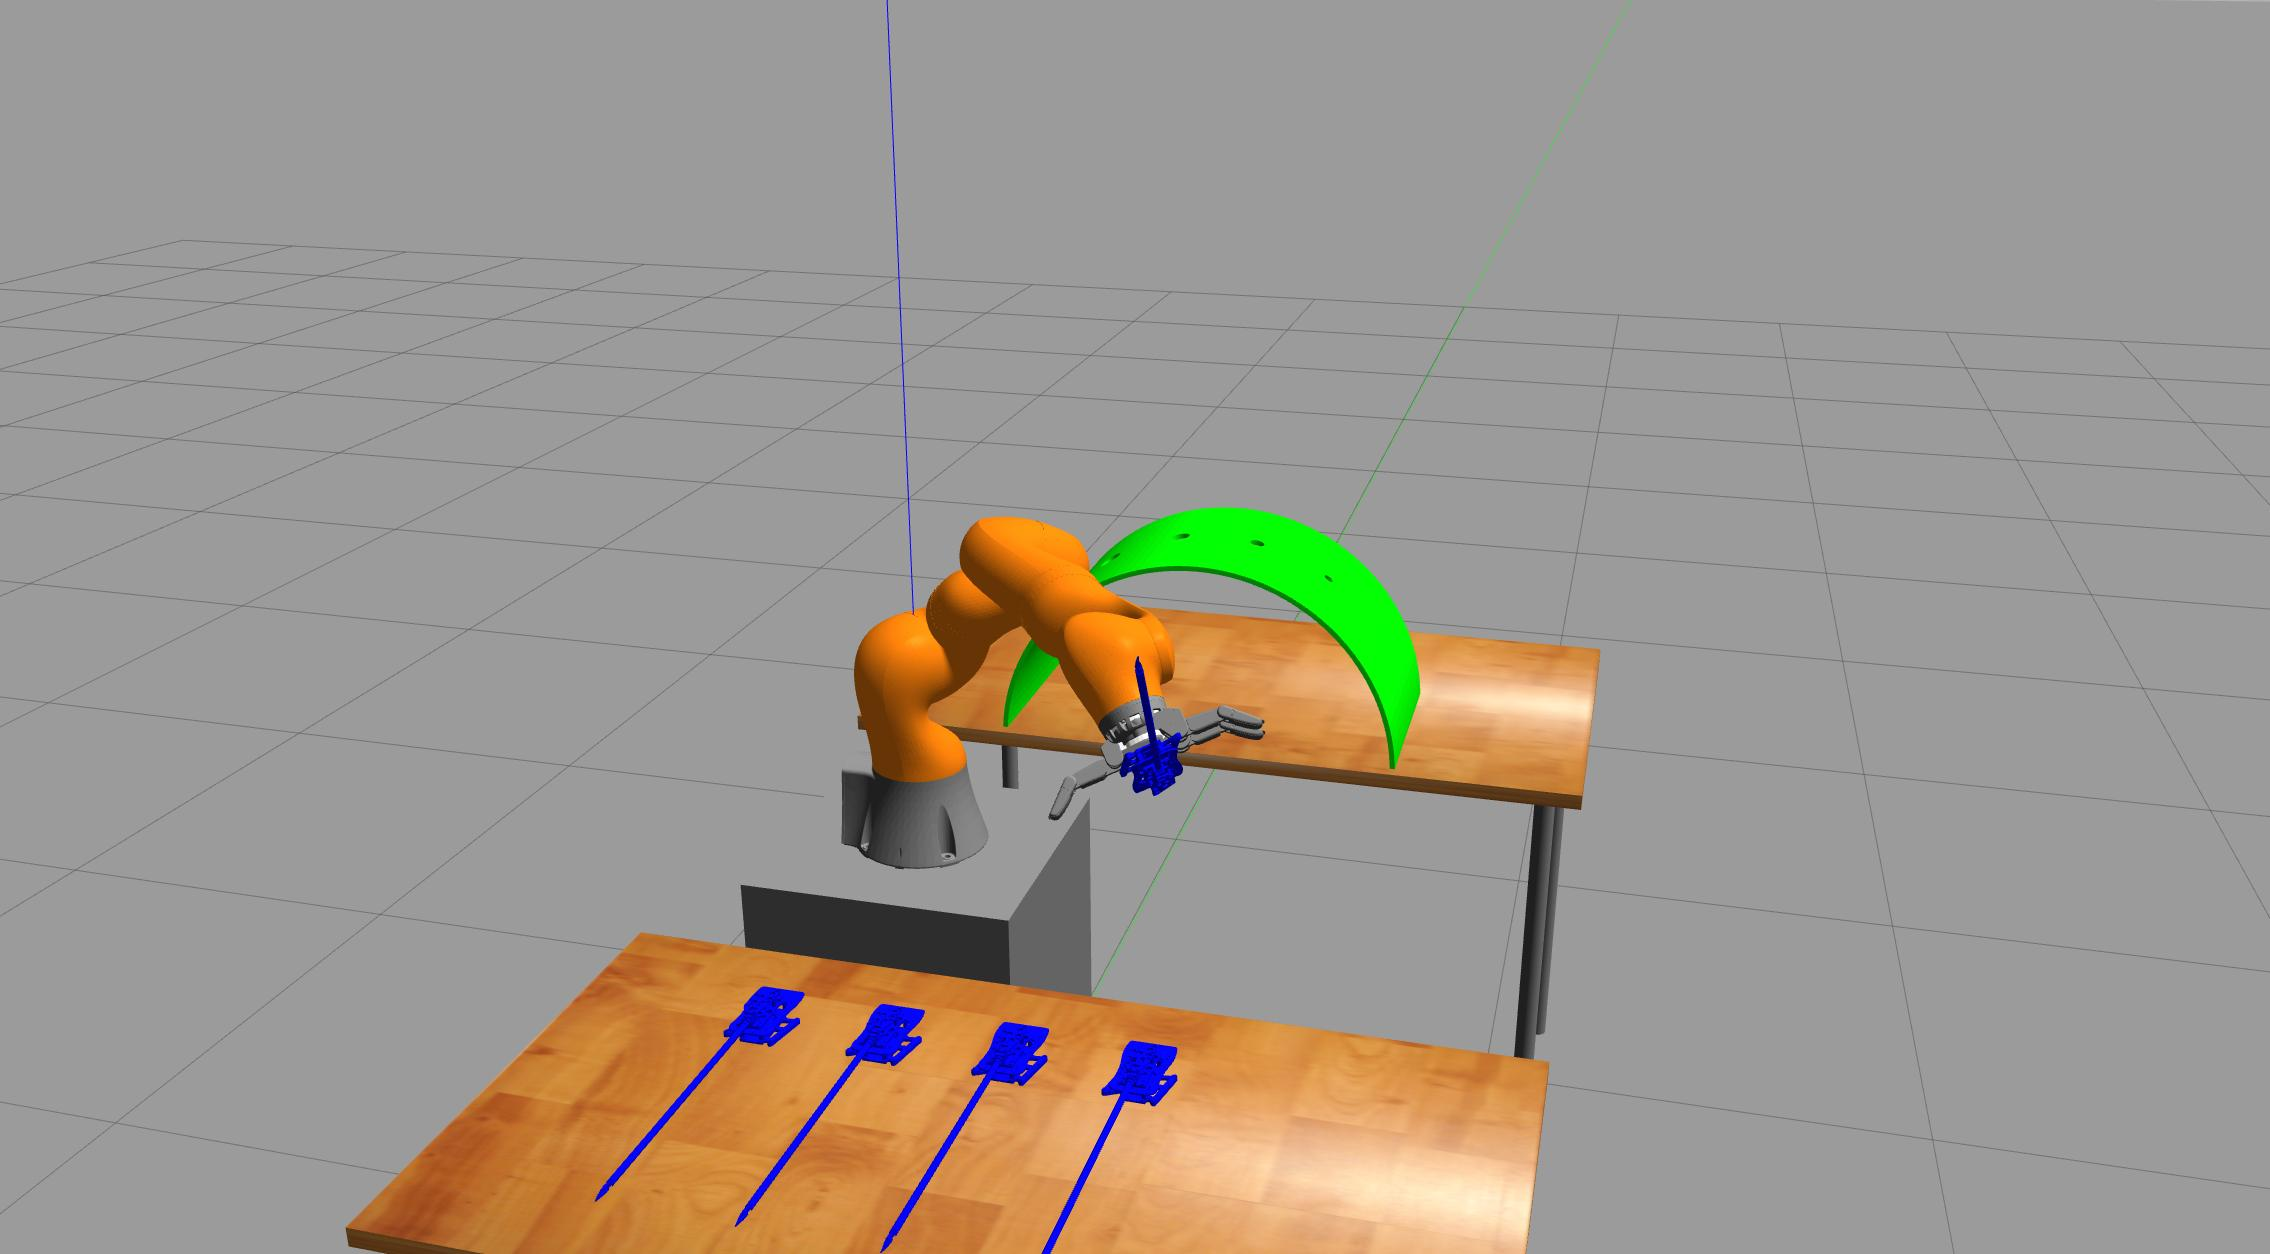
\includegraphics[width=0.3\textwidth]{images/robot_planner1/robot_planner1_3}\\
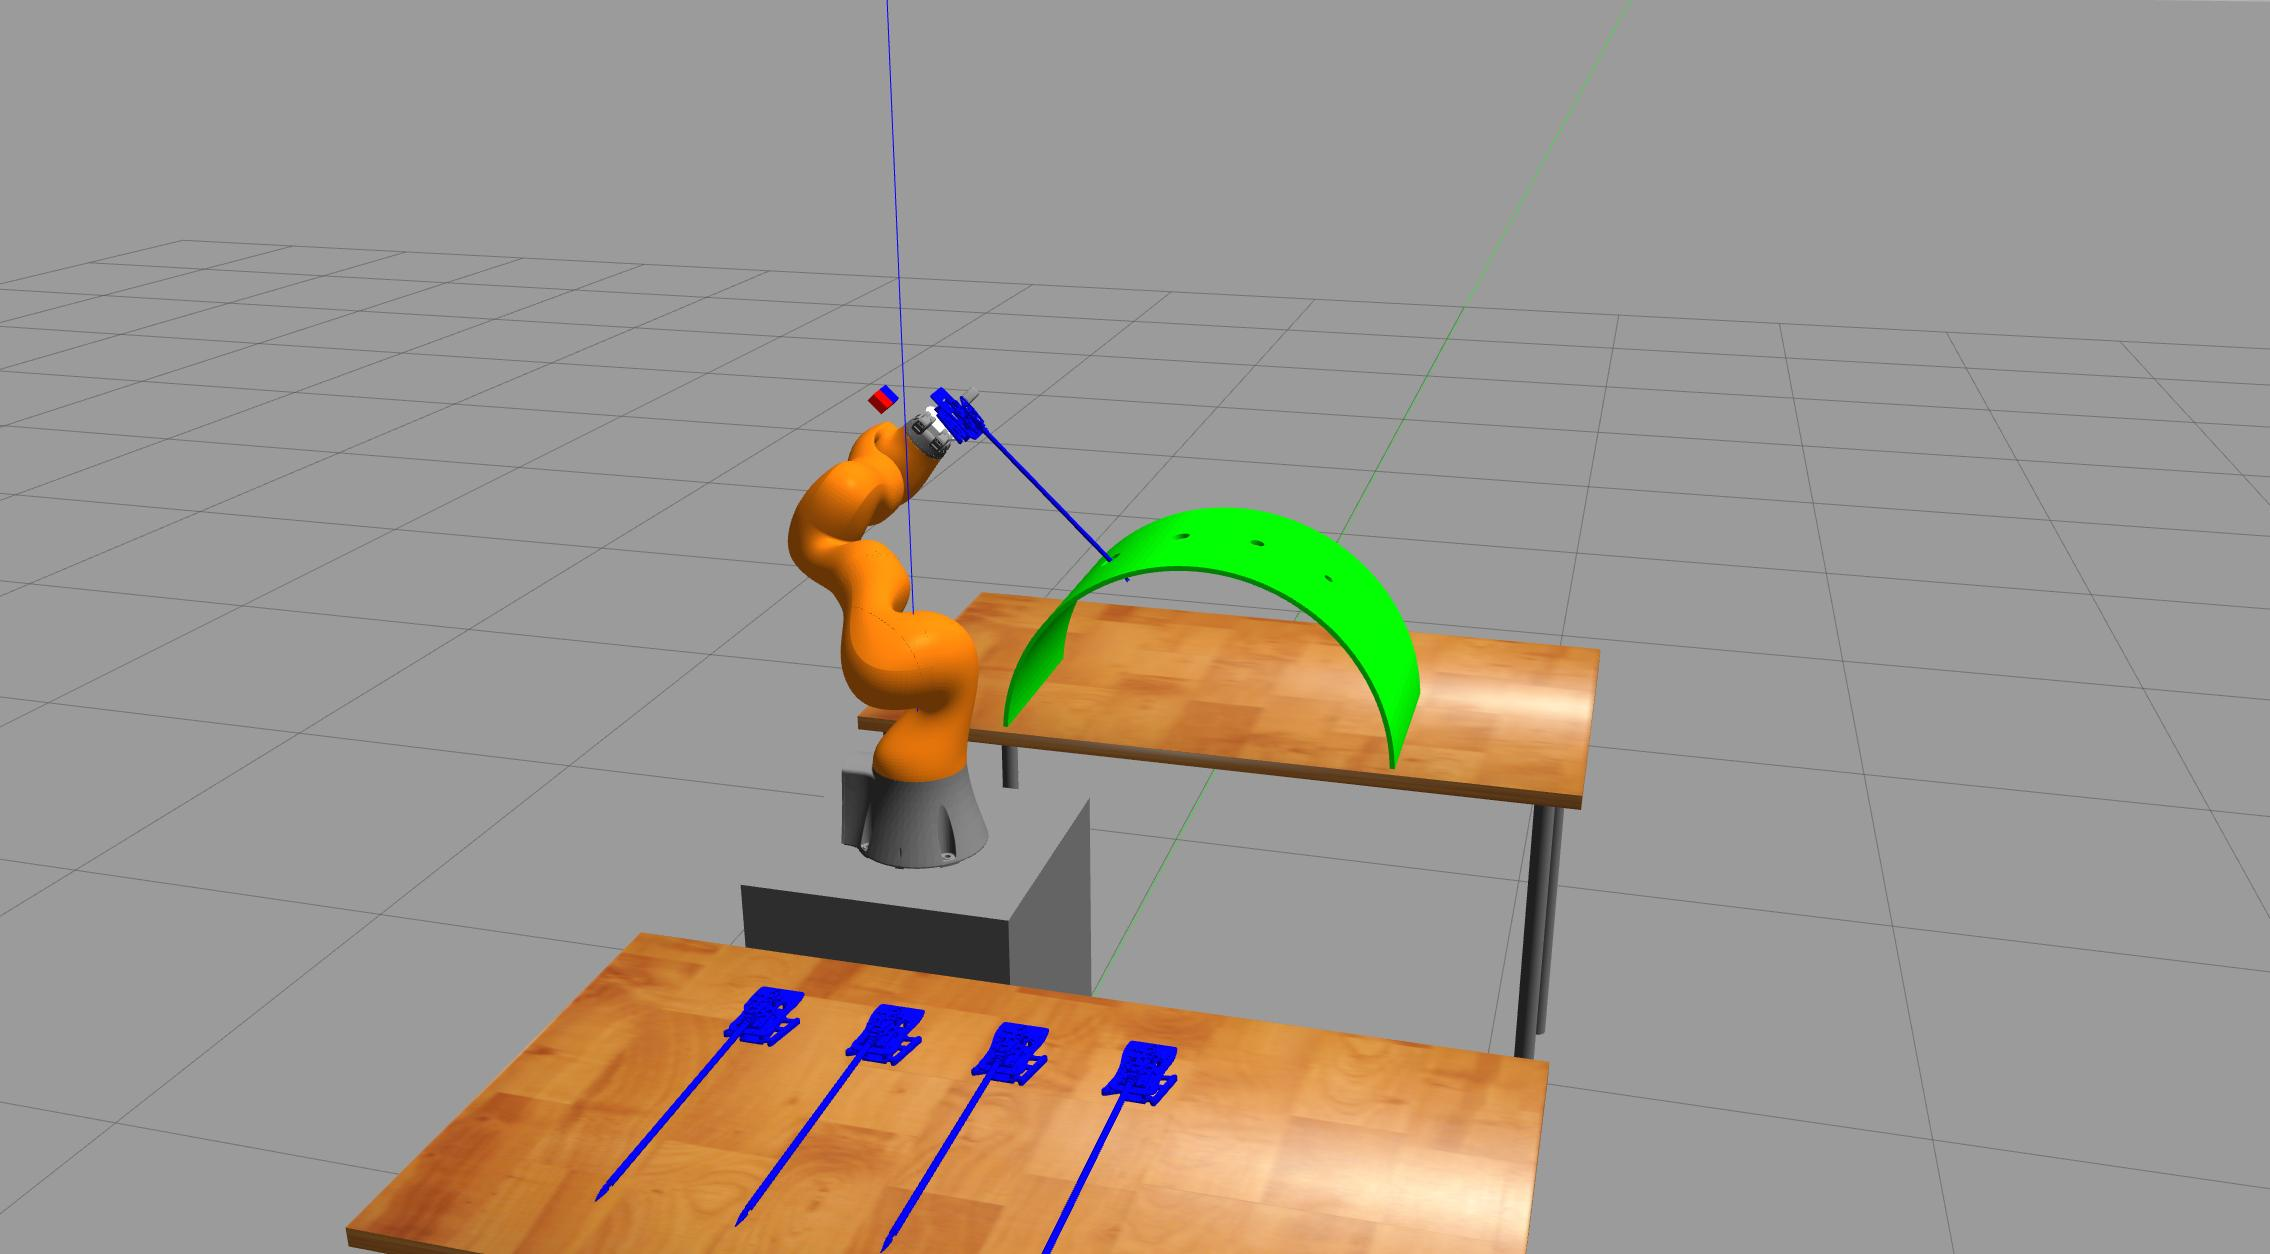
\includegraphics[width=0.3\textwidth]{images/robot_planner1/robot_planner1_4}
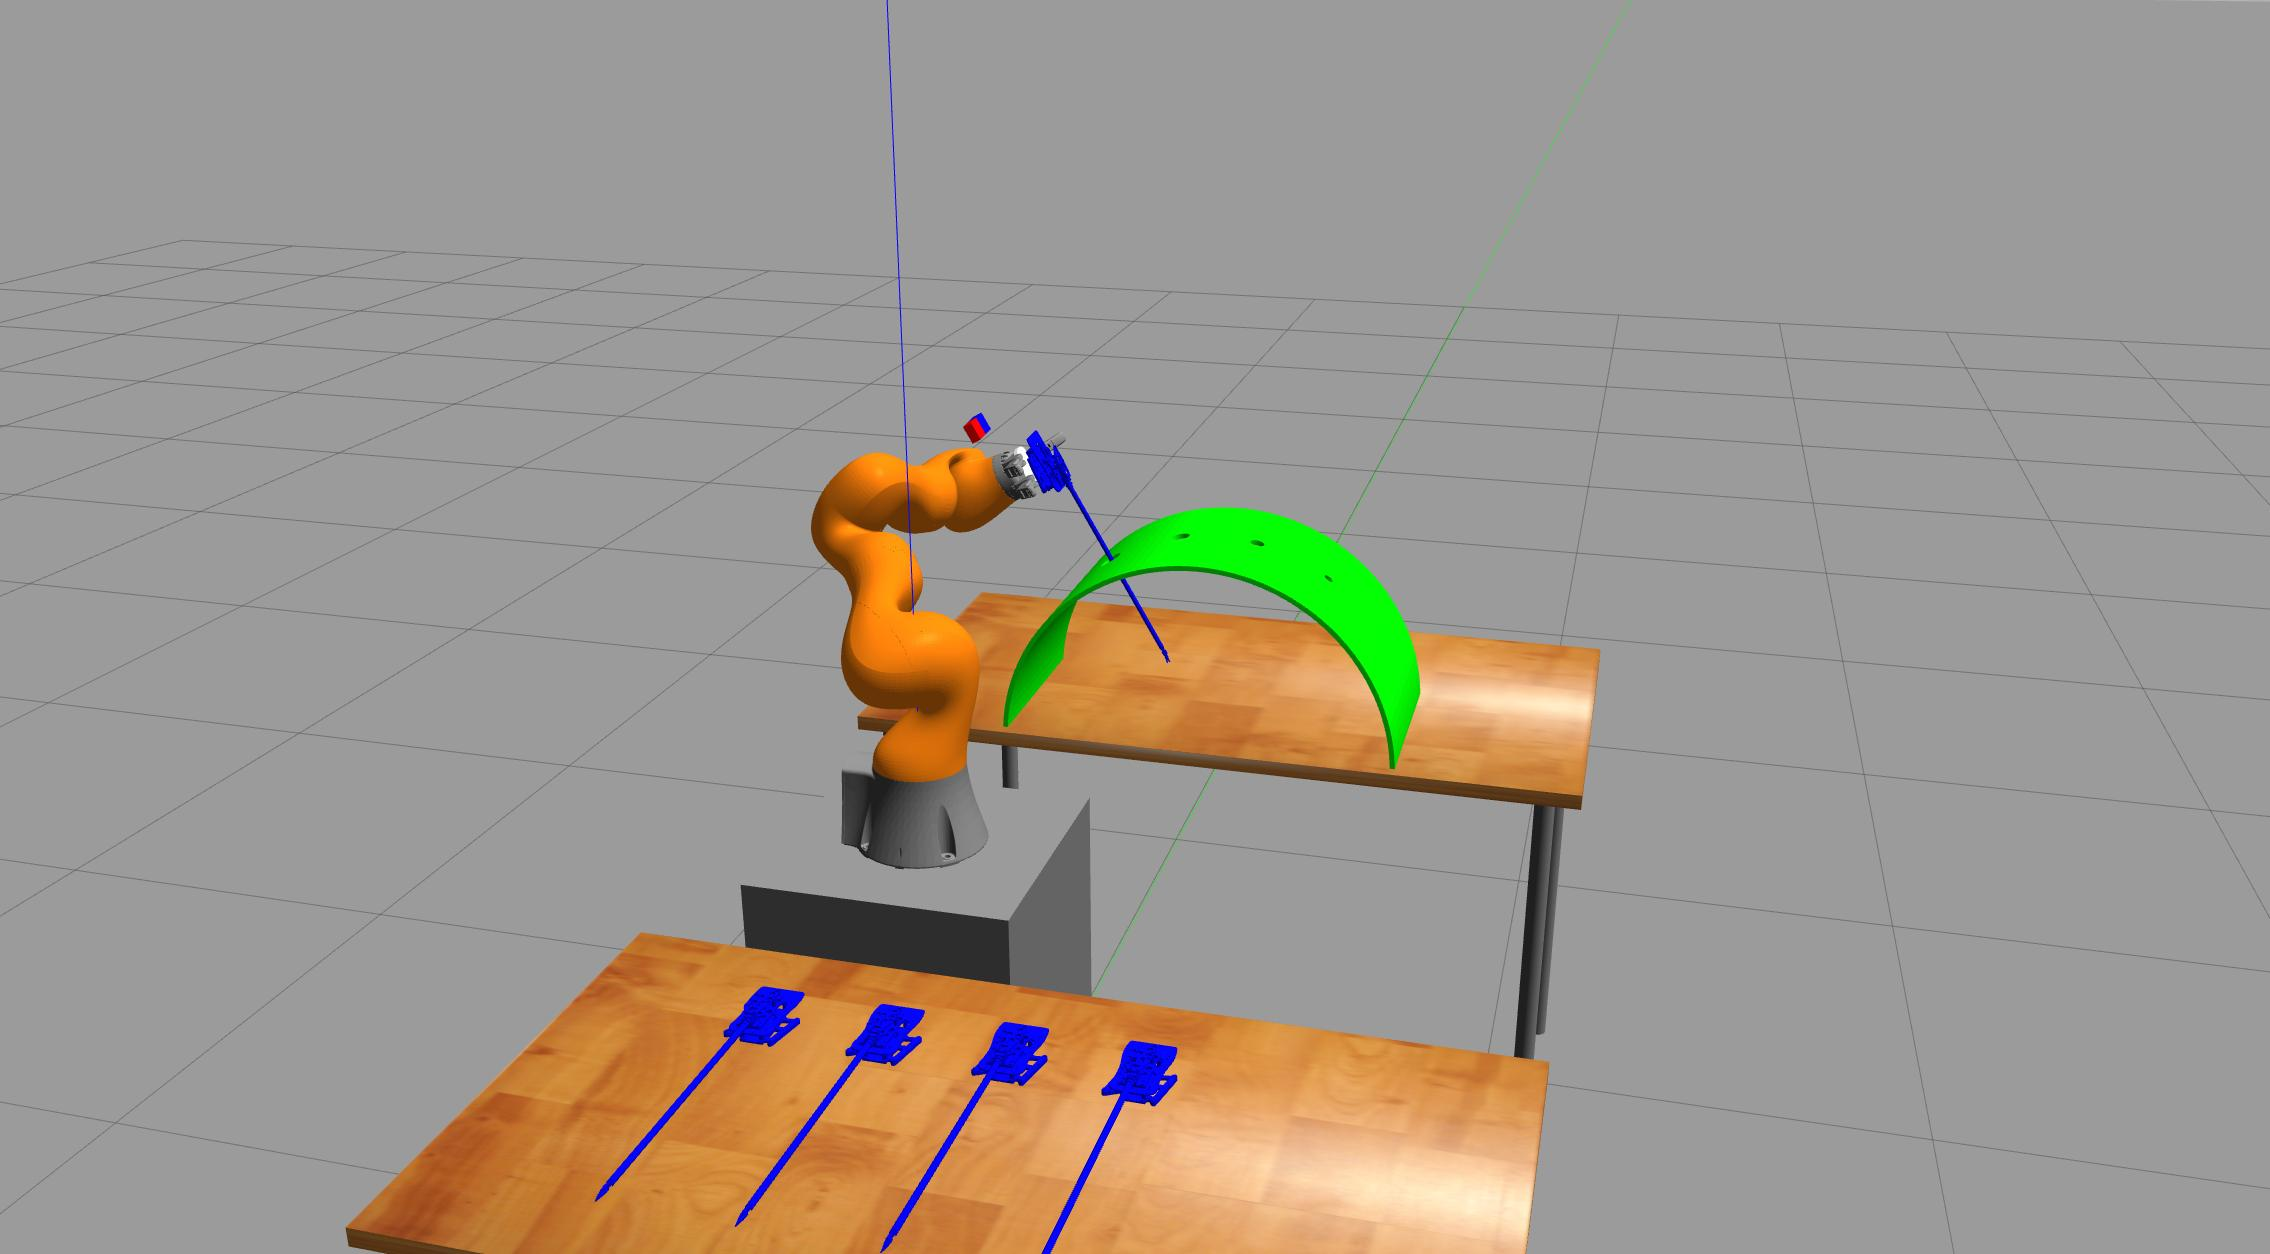
\includegraphics[width=0.3\textwidth]{images/robot_planner1/robot_planner1_5}
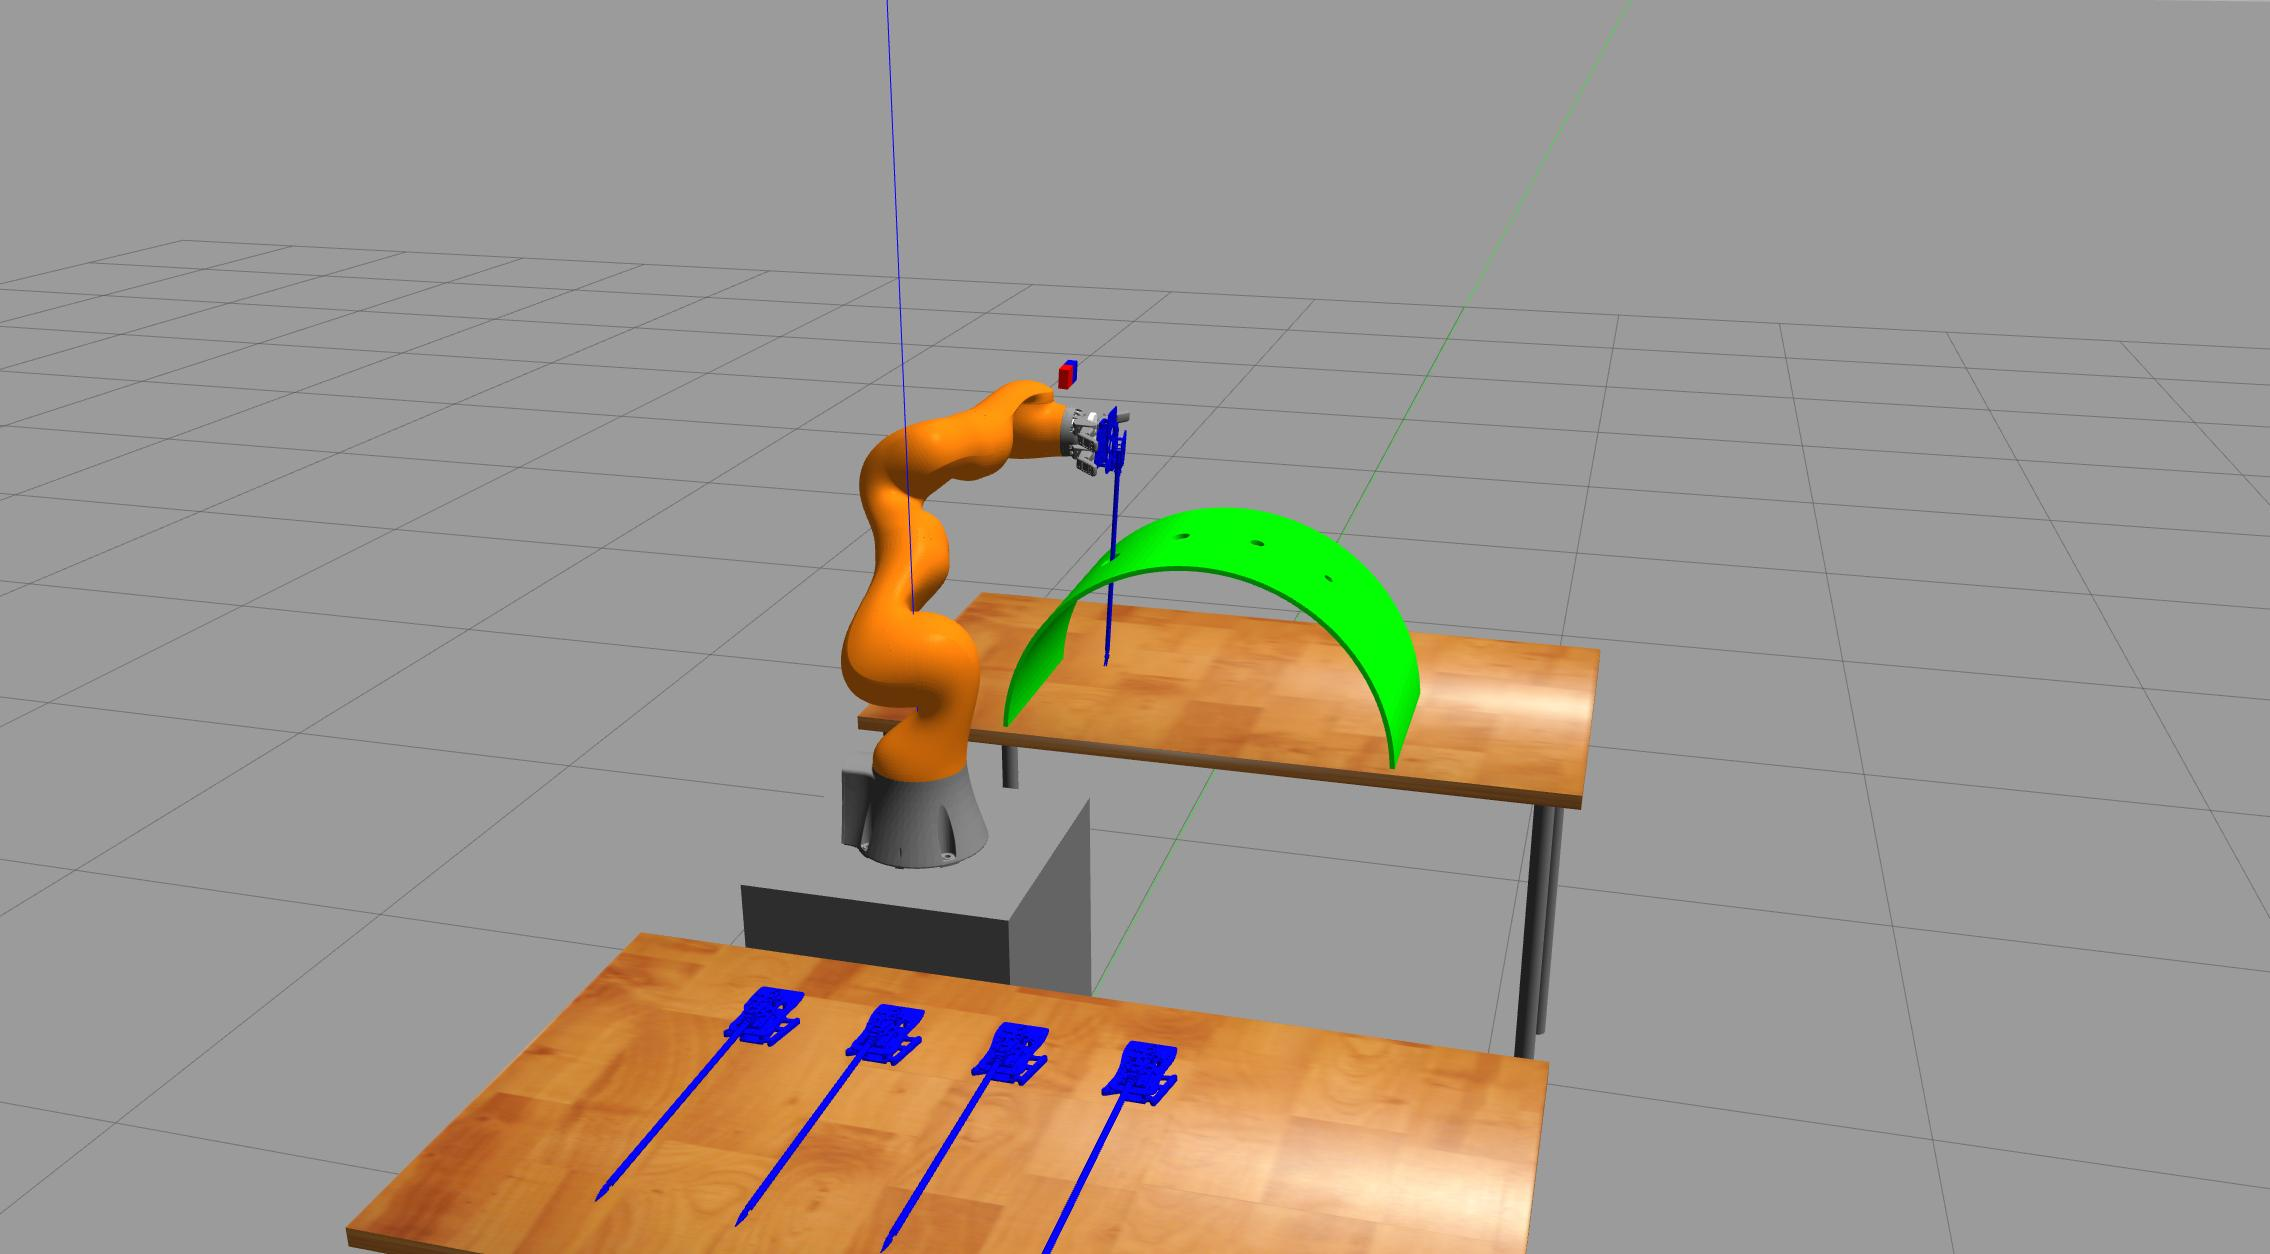
\includegraphics[width=0.3\textwidth]{images/robot_planner1/robot_planner1_6}\\
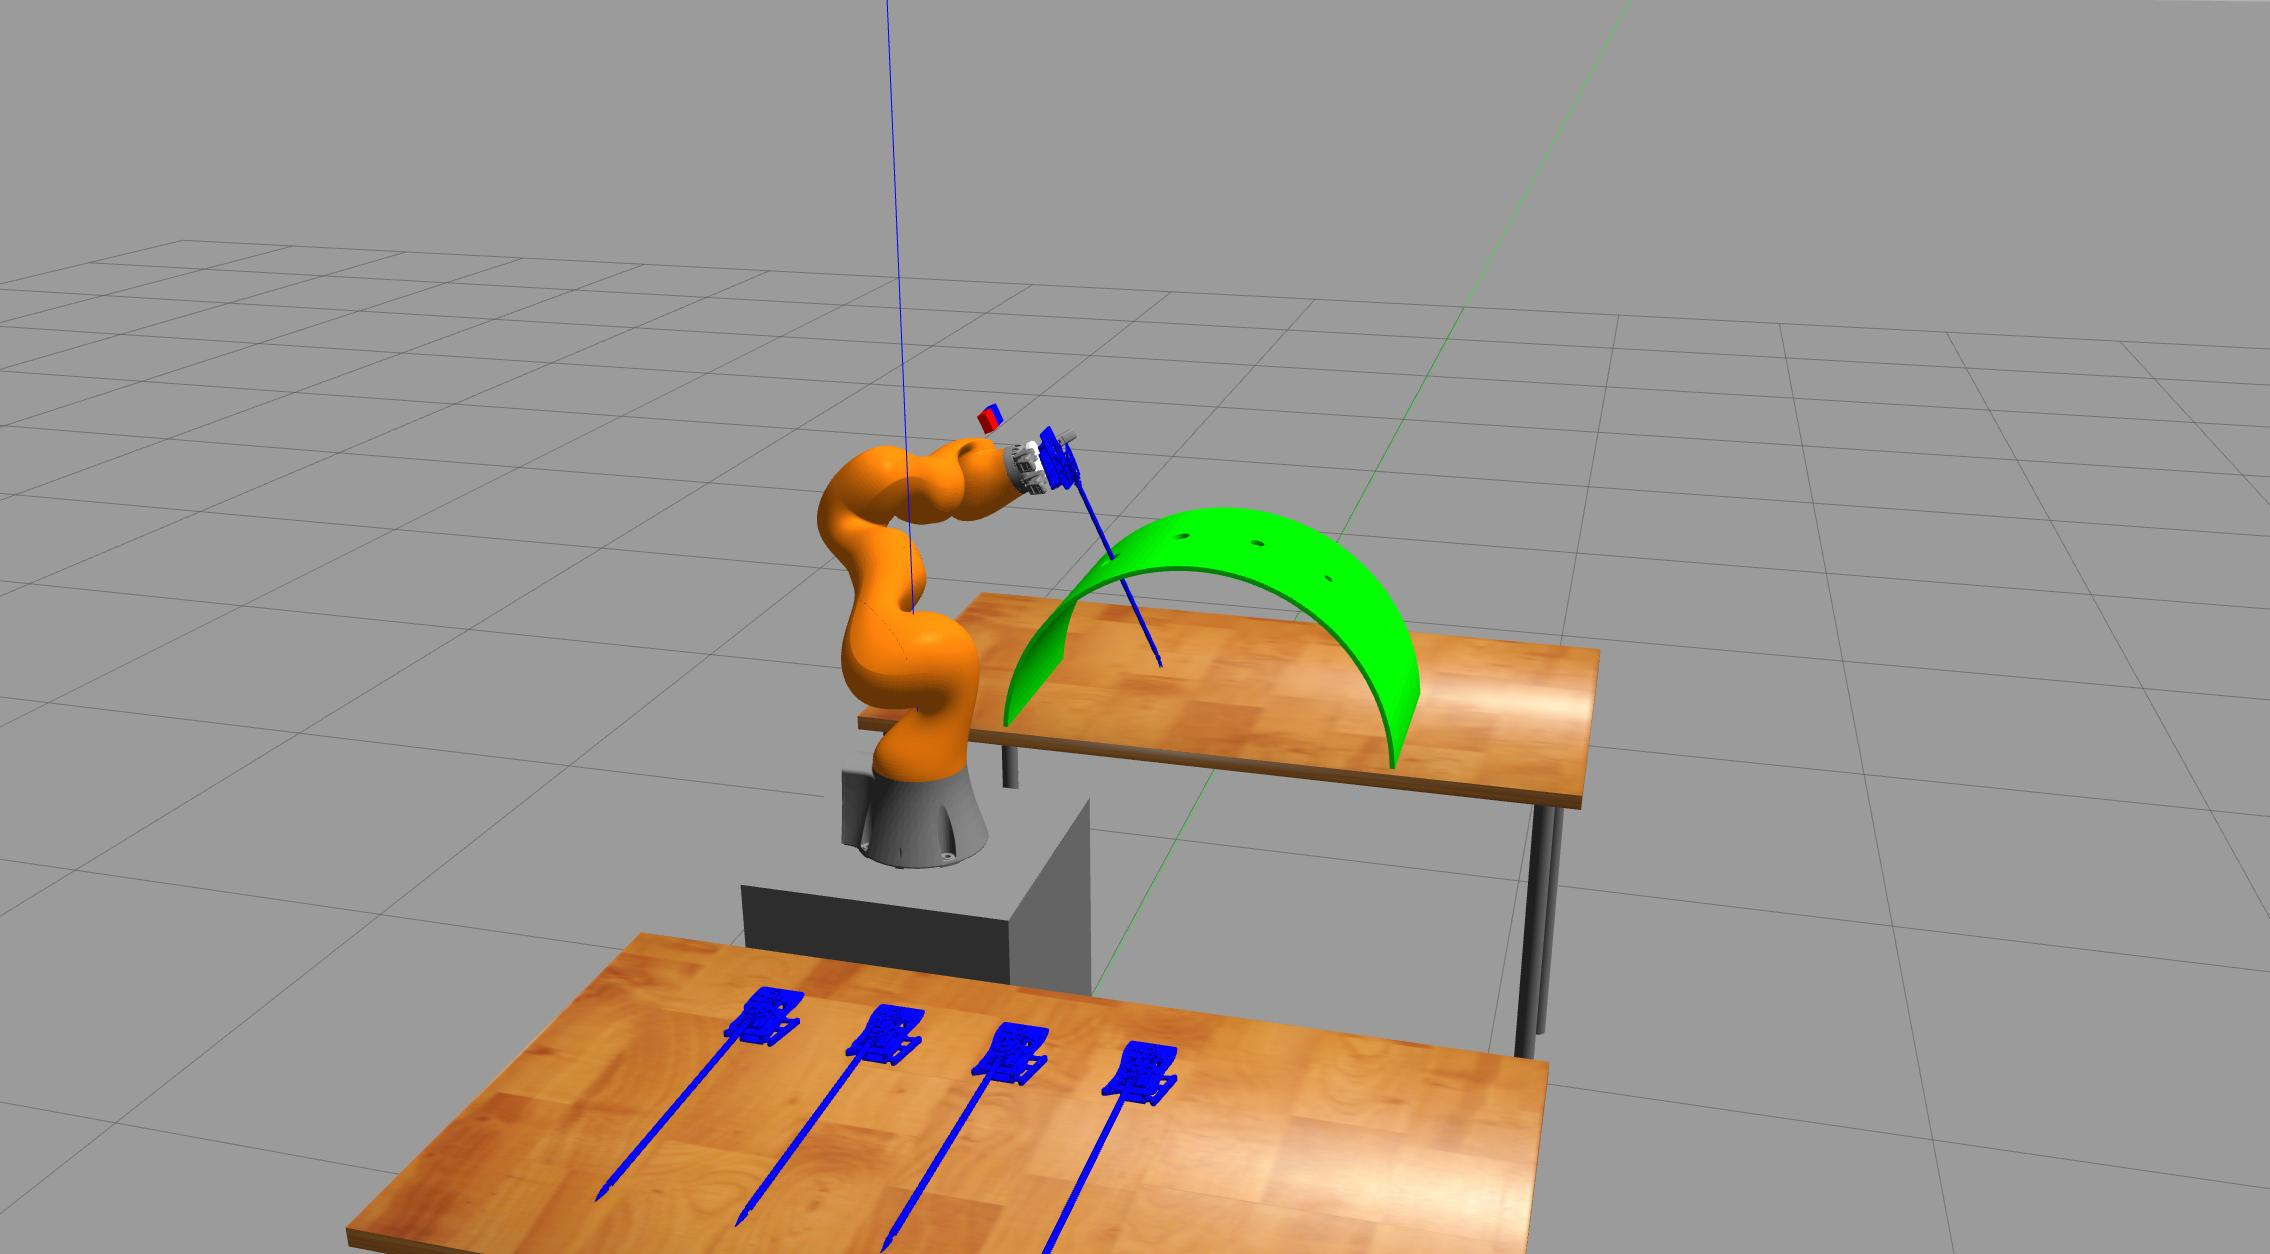
\includegraphics[width=0.3\textwidth]{images/robot_planner1/robot_planner1_7}
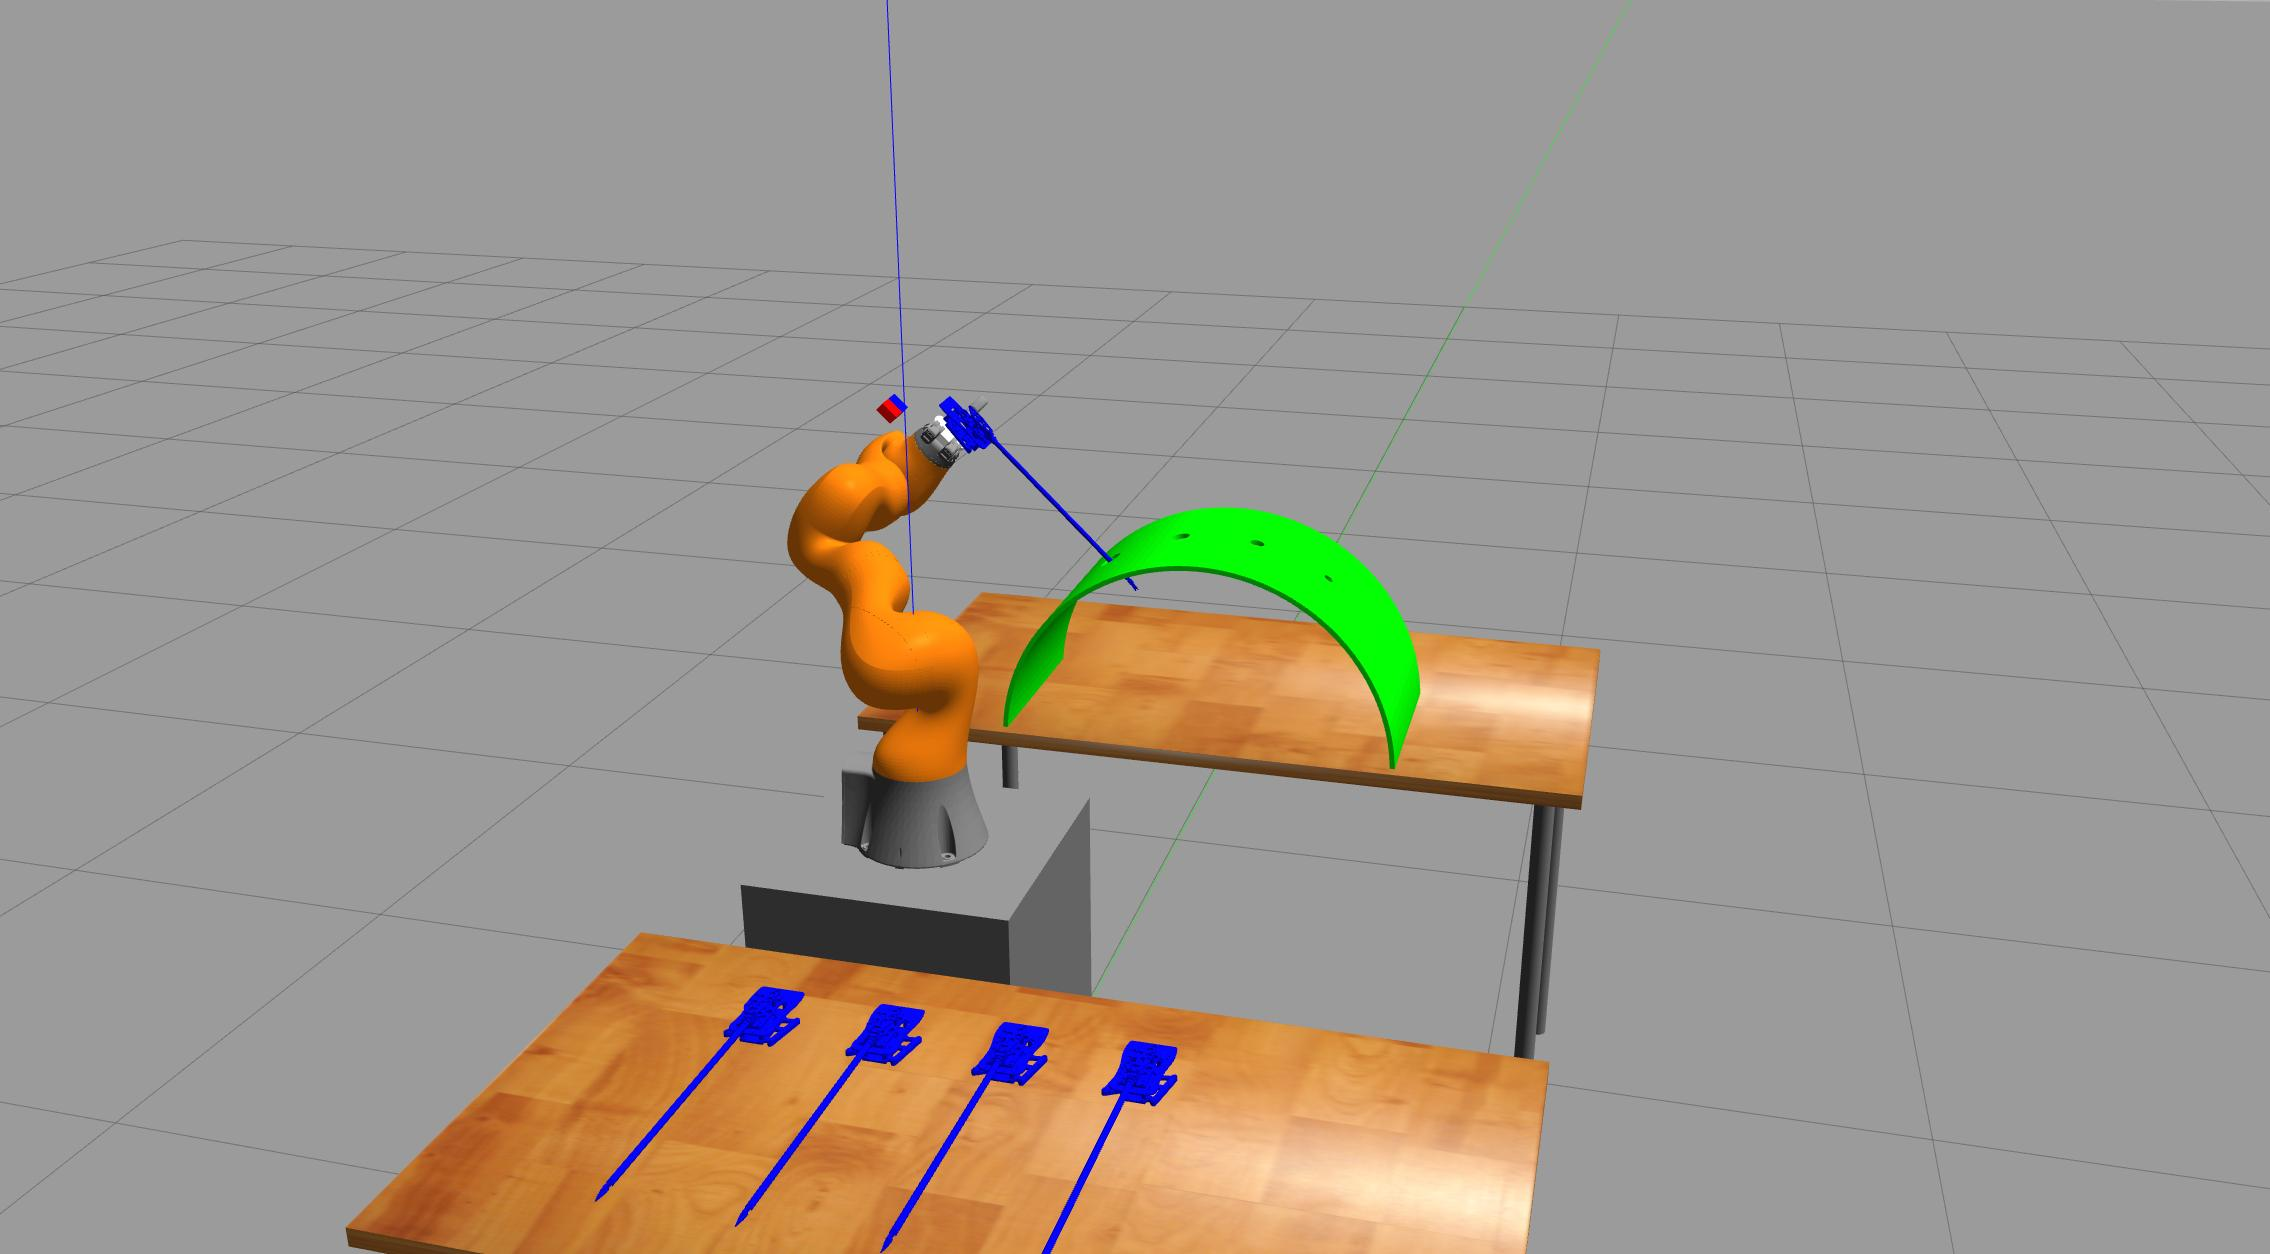
\includegraphics[width=0.3\textwidth]{images/robot_planner1/robot_planner1_8}
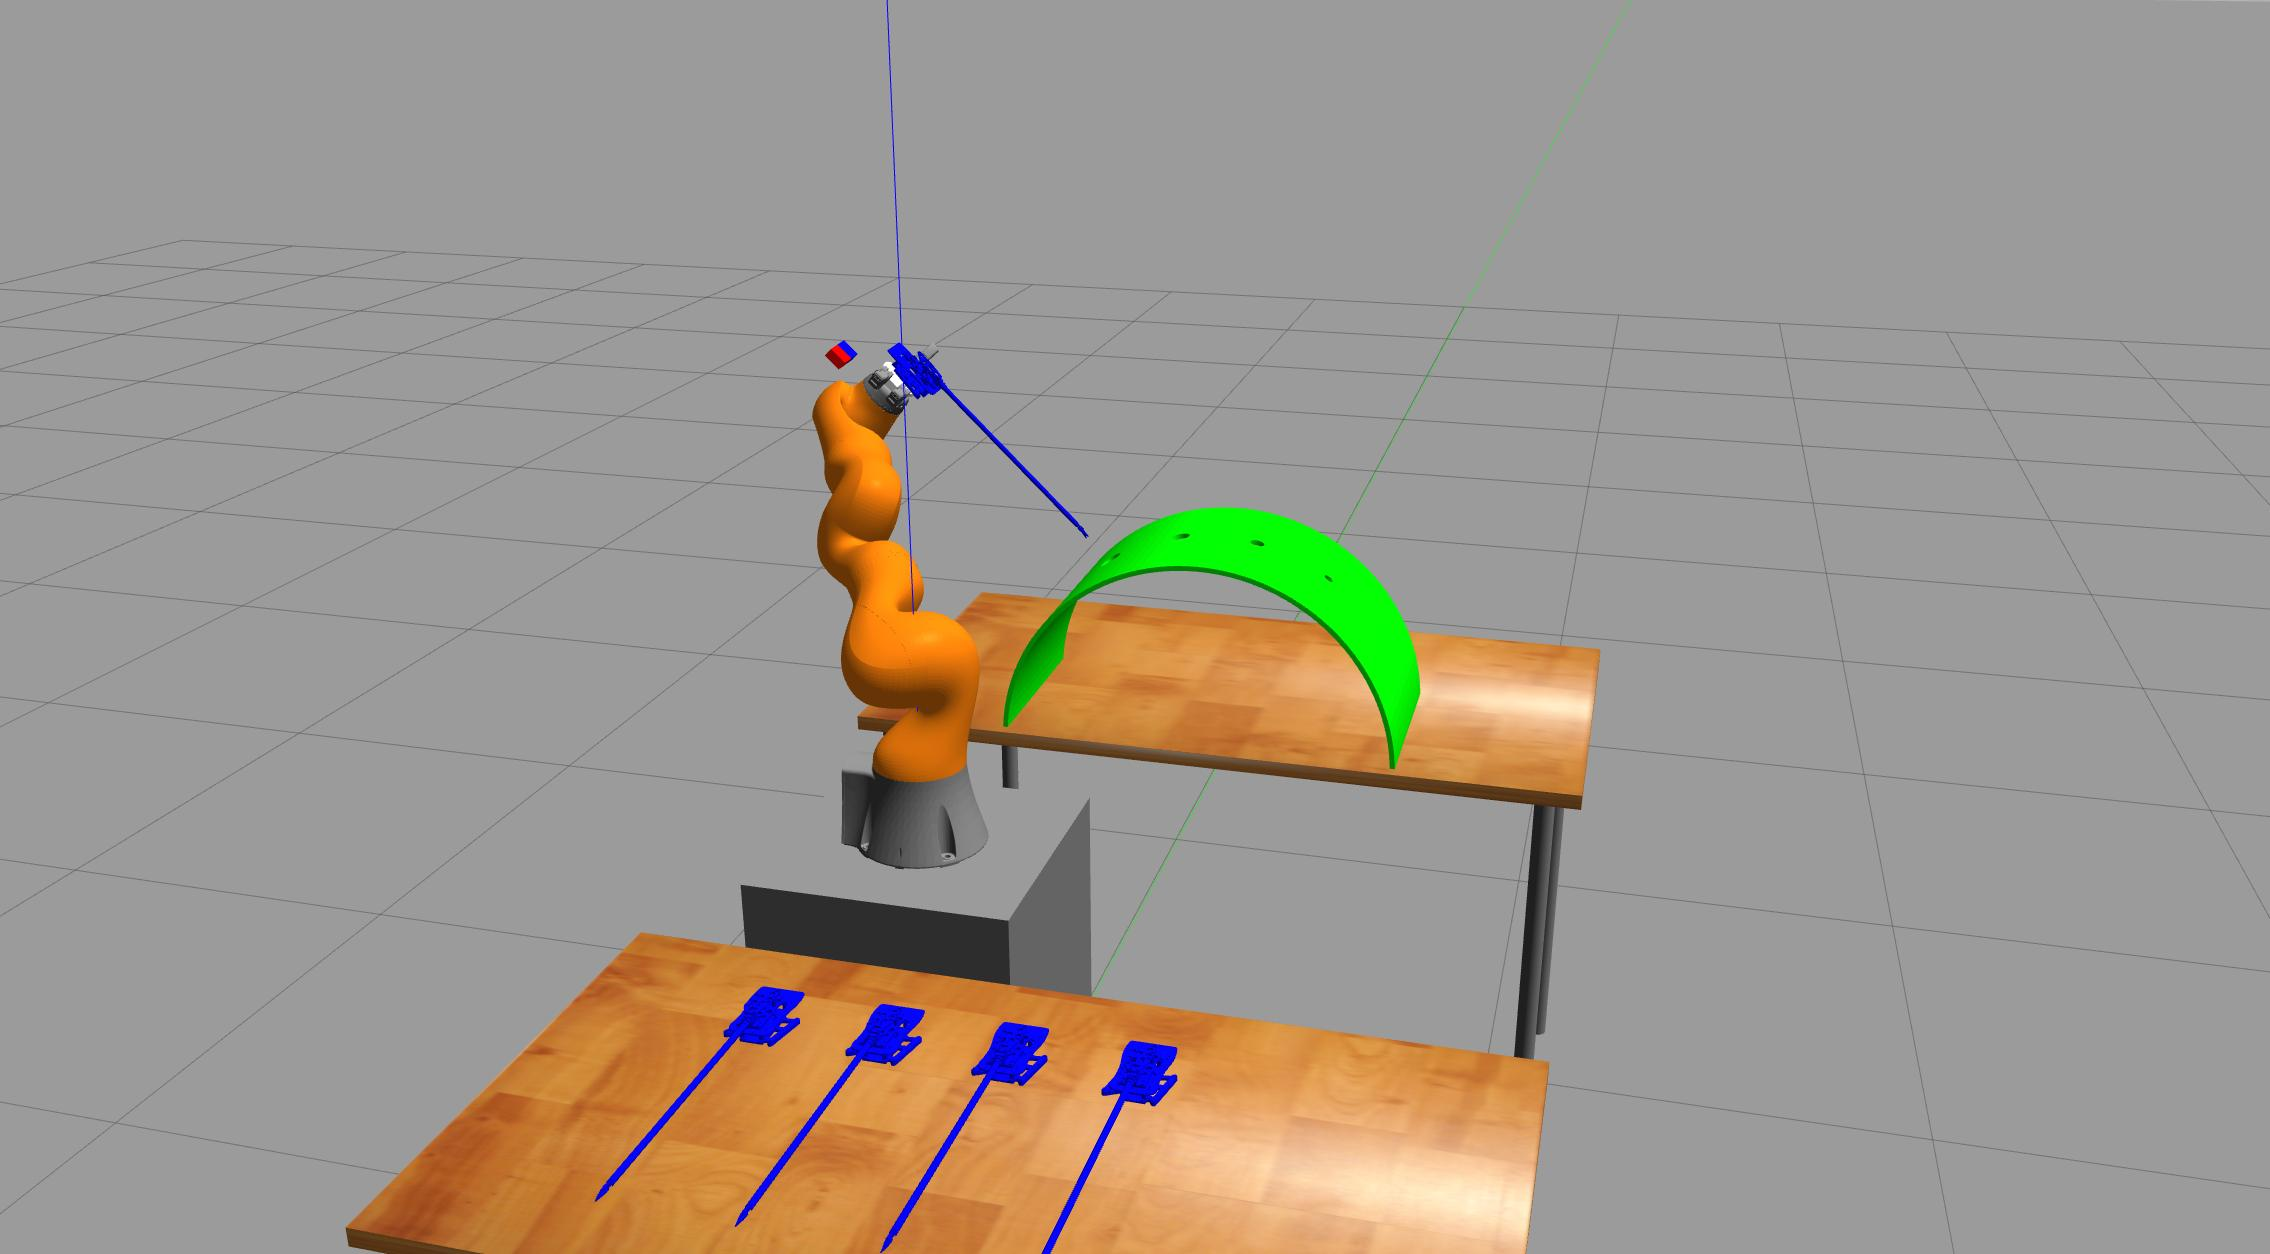
\includegraphics[width=0.3\textwidth]{images/robot_planner1/robot_planner1_9}\\
\caption{Experiment 1:}
\end{figure}
\end{center}


\subsubsection{Robot Planner 2}

In this experiment, we plan a path such that the robot arm will visit all holes of the mounting dock and will try the insertion movement of the surgical tool.
This experiment is very useful, because it shows whether all holes of the mounting dock are \textbf{reachable} (inside the robot's work space) and if so, how 
\textbf{dexterous} the robot will be in pivoting around each hole, i.e. how free the robot arm is to execute pivot motions.

\begin{center}
\begin{figure}[H]
\centering
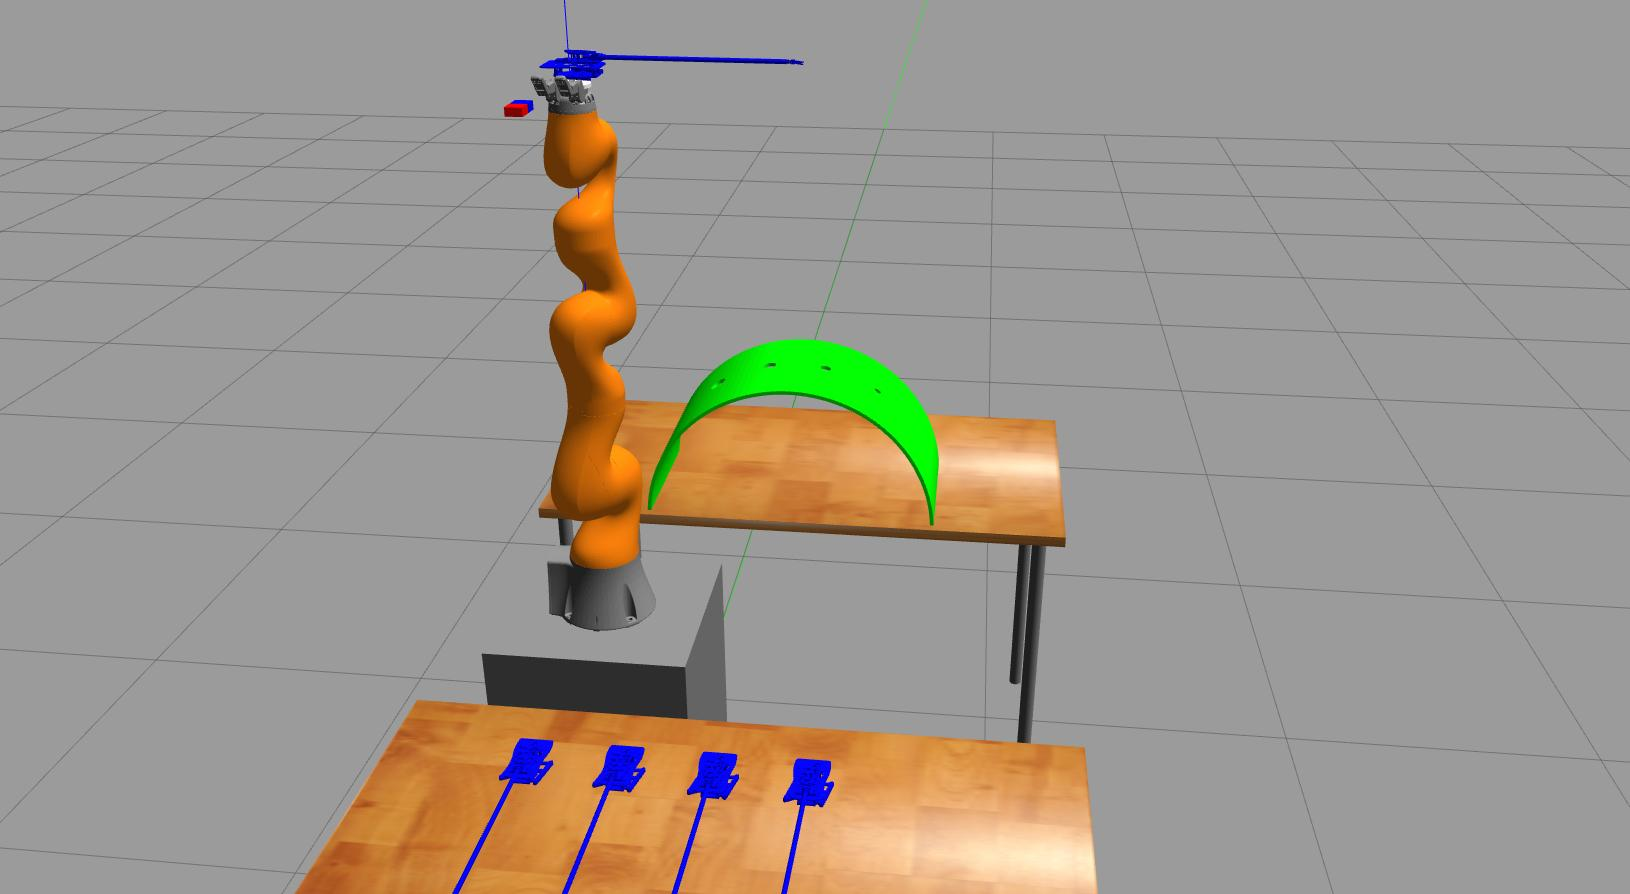
\includegraphics[width=0.3\textwidth]{images/robot_planner2/robot_planner2_1}
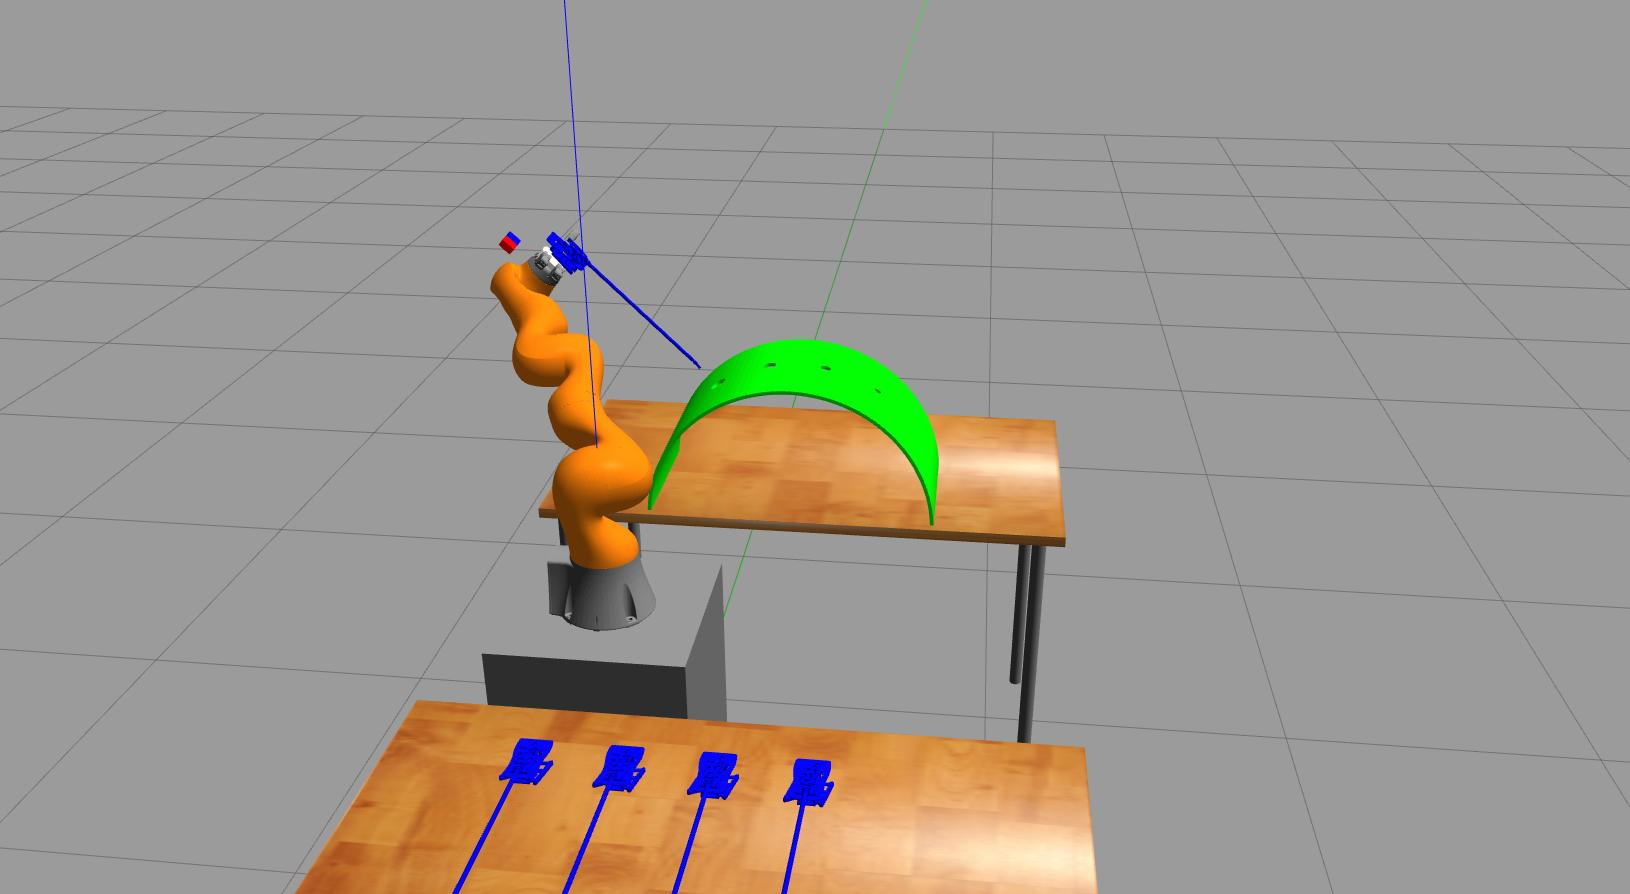
\includegraphics[width=0.3\textwidth]{images/robot_planner2/robot_planner2_2}
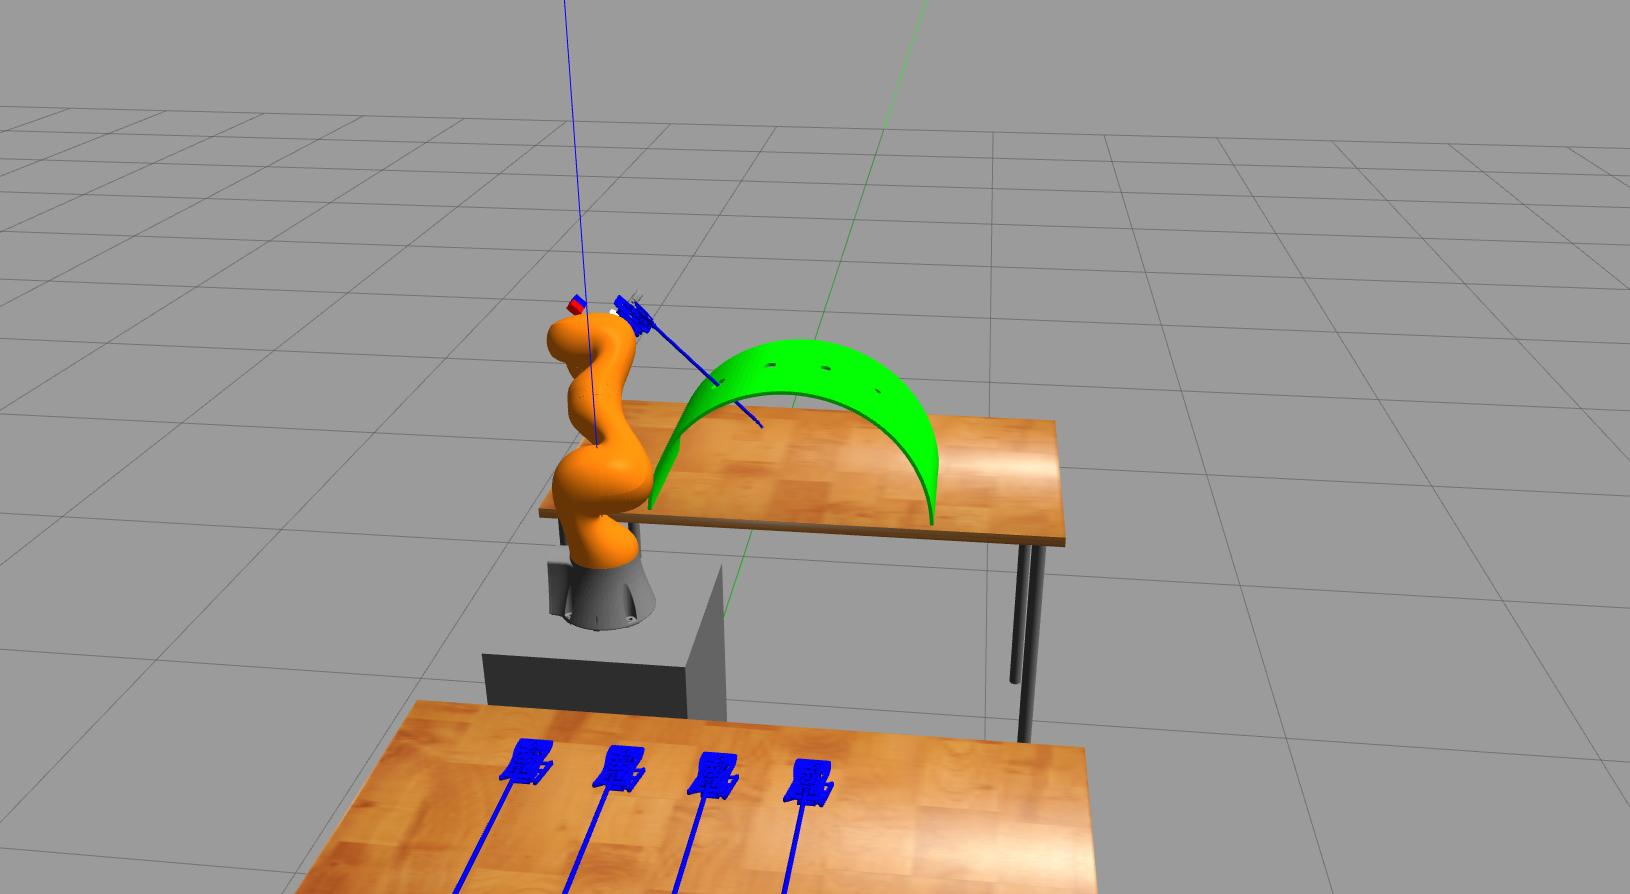
\includegraphics[width=0.3\textwidth]{images/robot_planner2/robot_planner2_3}\\
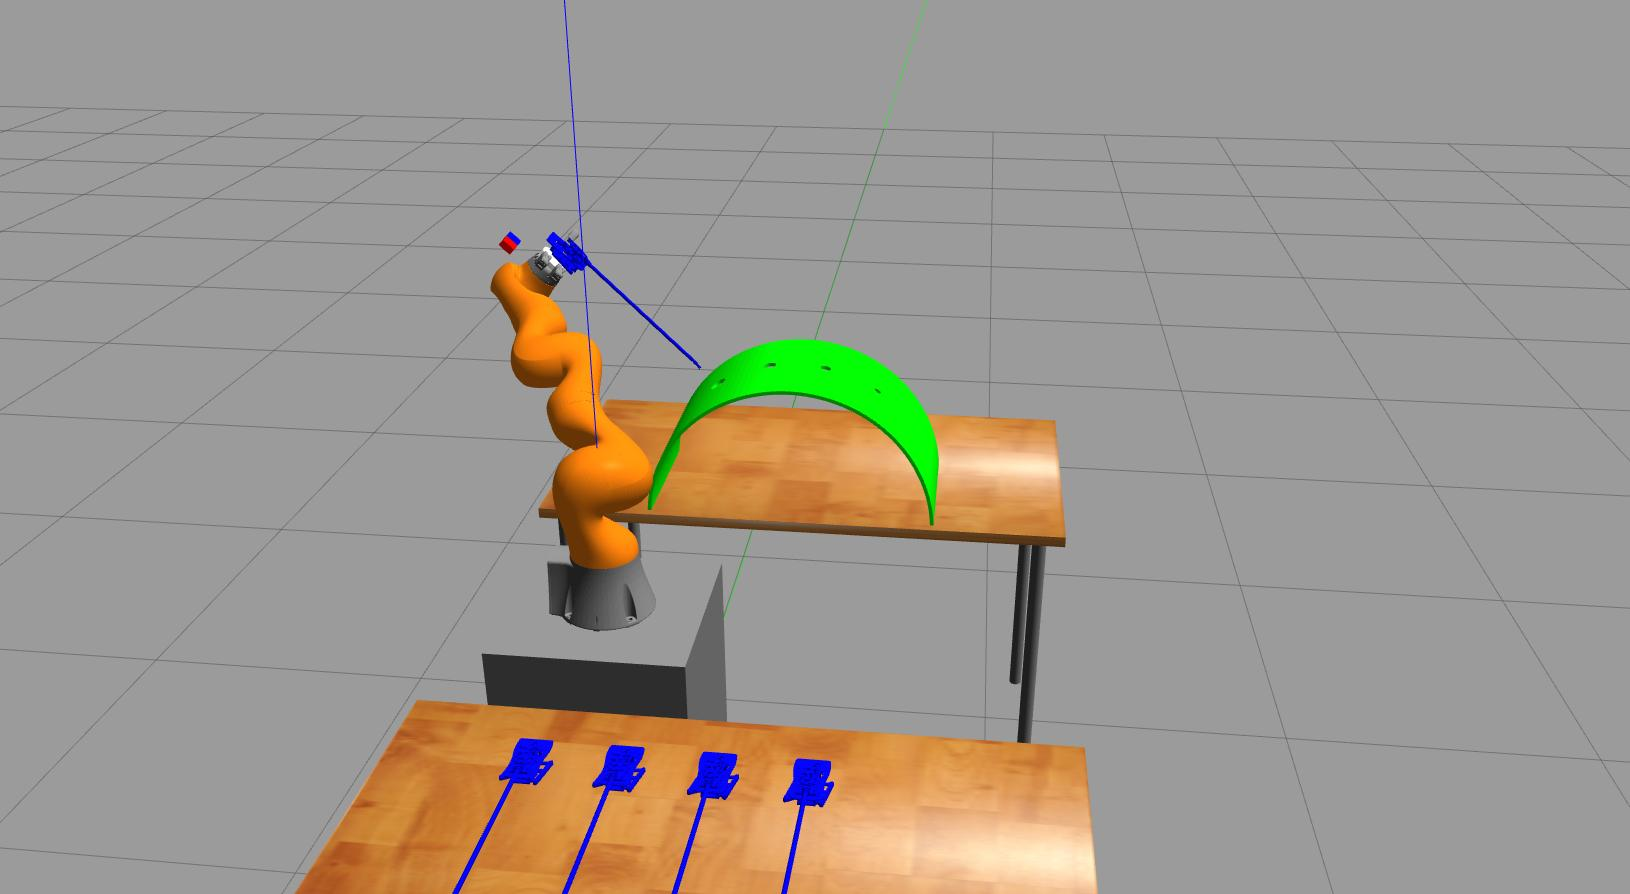
\includegraphics[width=0.3\textwidth]{images/robot_planner2/robot_planner2_4}
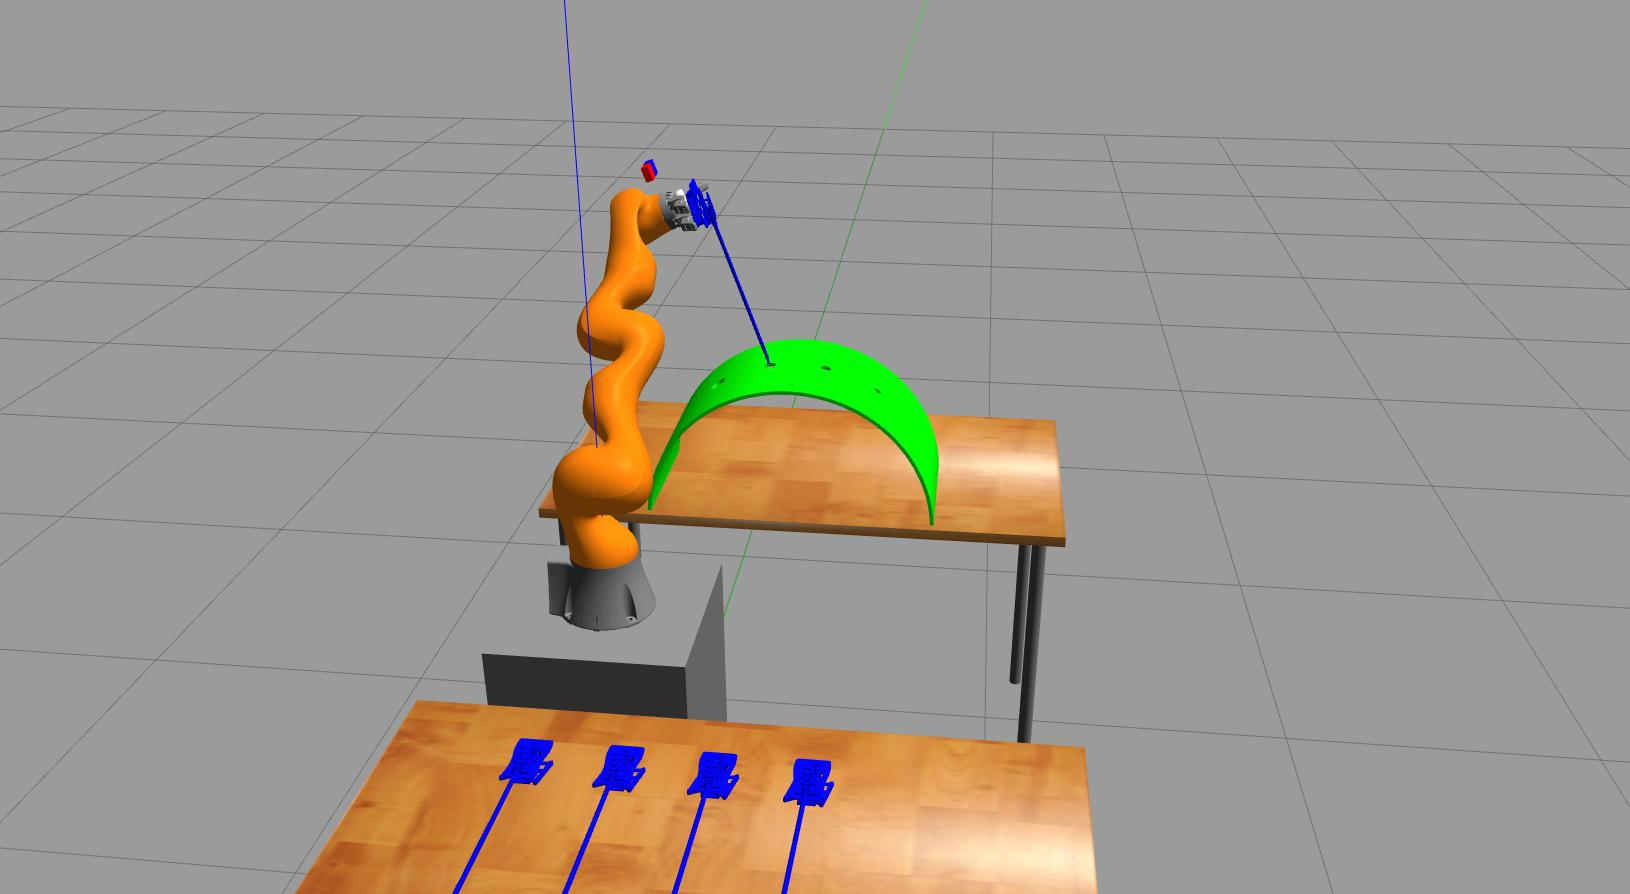
\includegraphics[width=0.3\textwidth]{images/robot_planner2/robot_planner2_5}
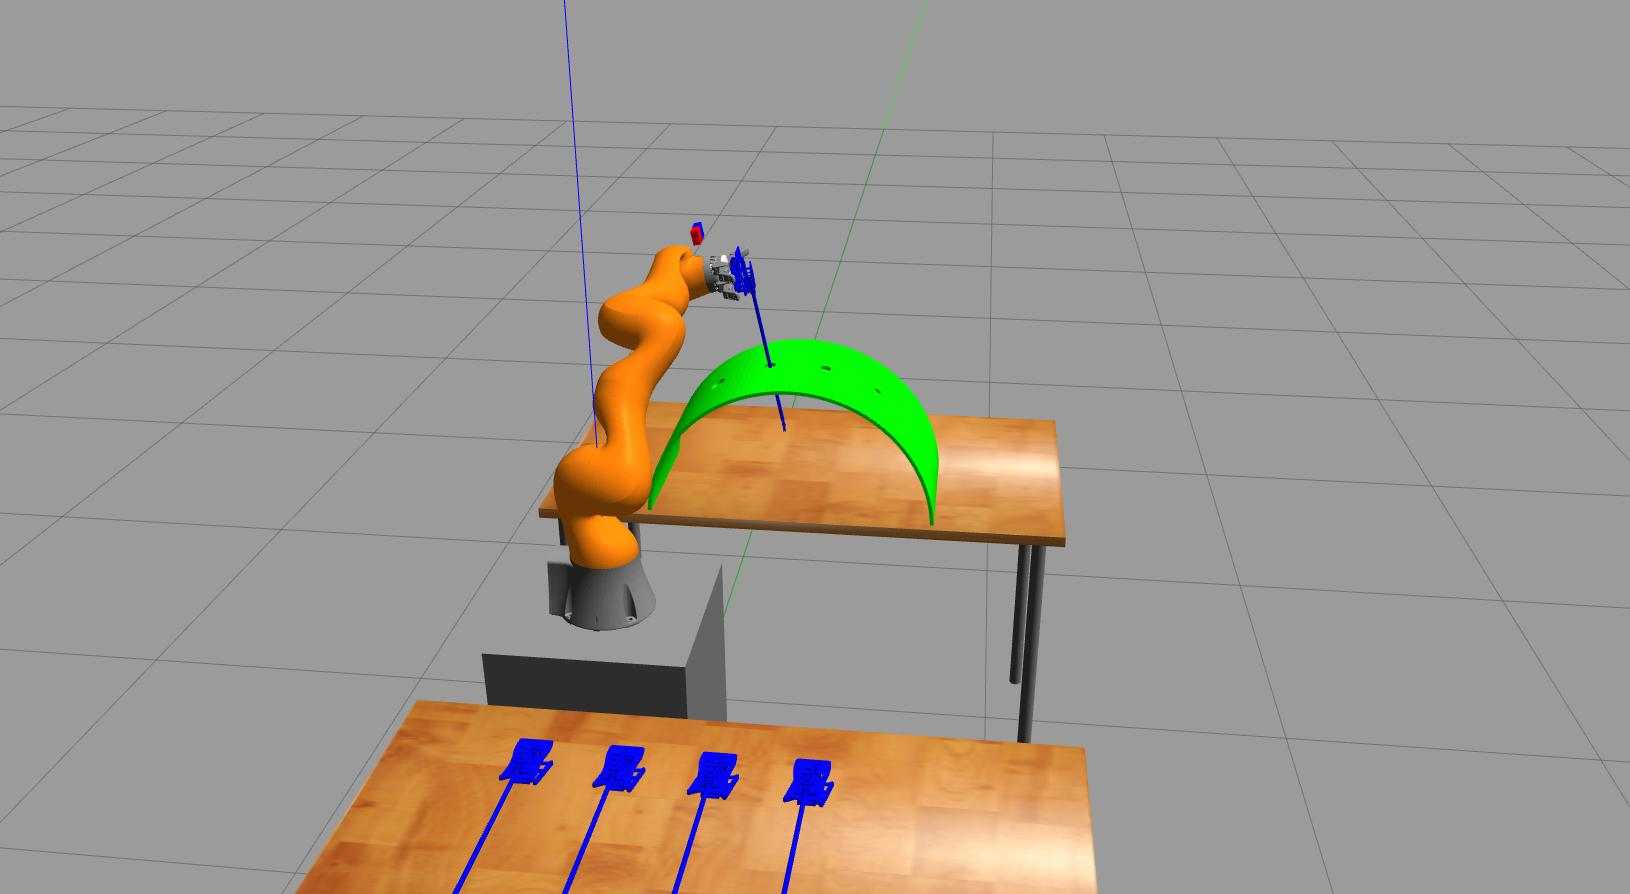
\includegraphics[width=0.3\textwidth]{images/robot_planner2/robot_planner2_6}\\
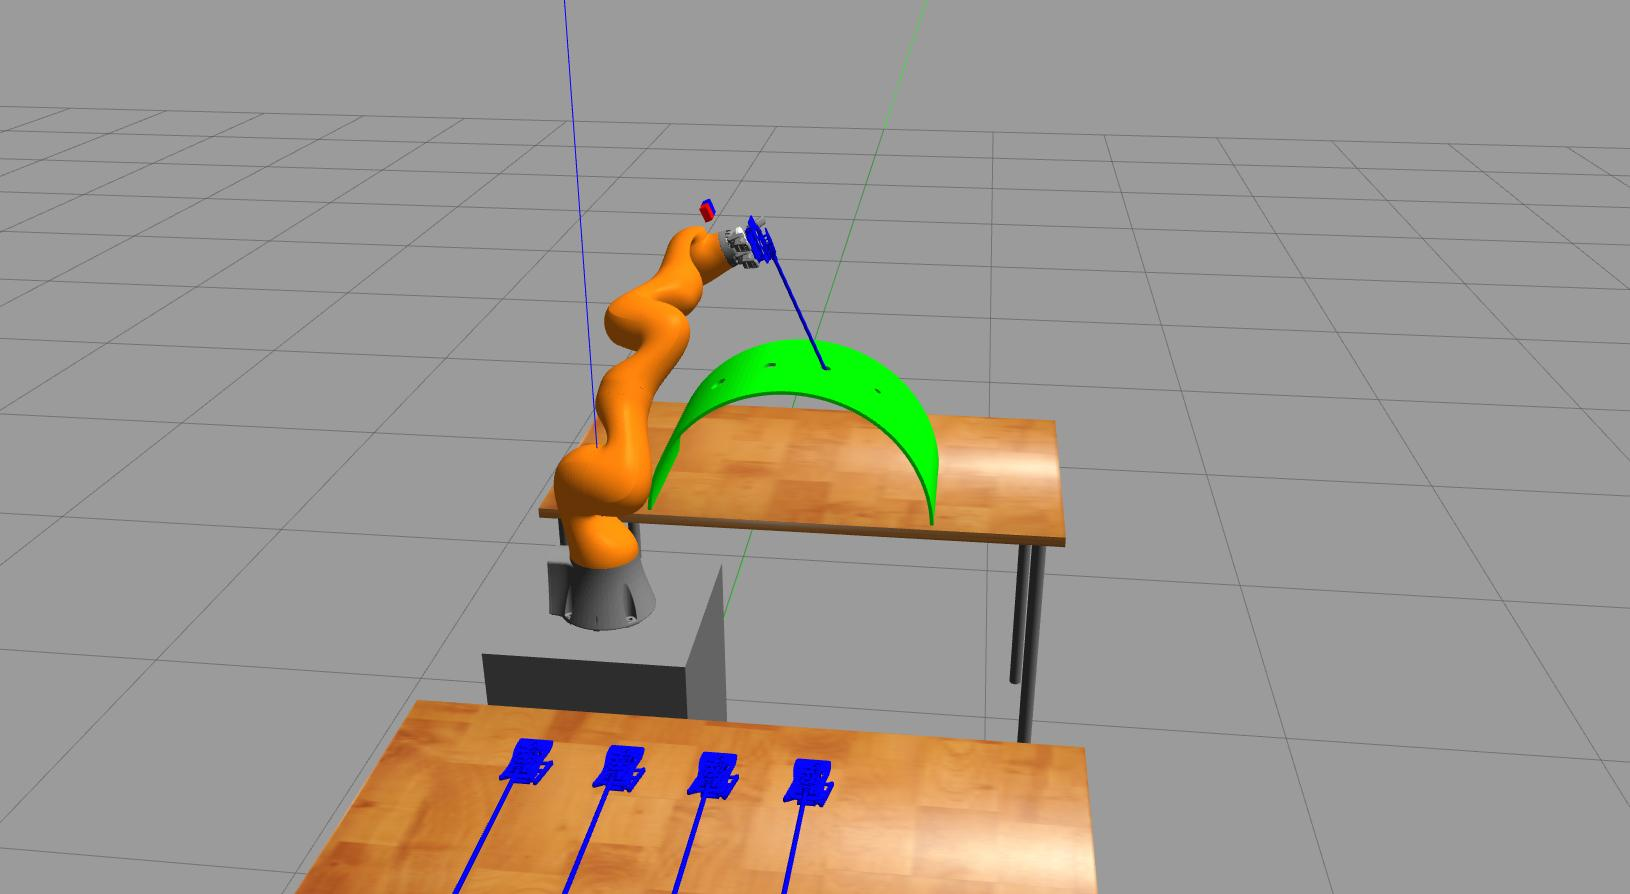
\includegraphics[width=0.3\textwidth]{images/robot_planner2/robot_planner2_7}
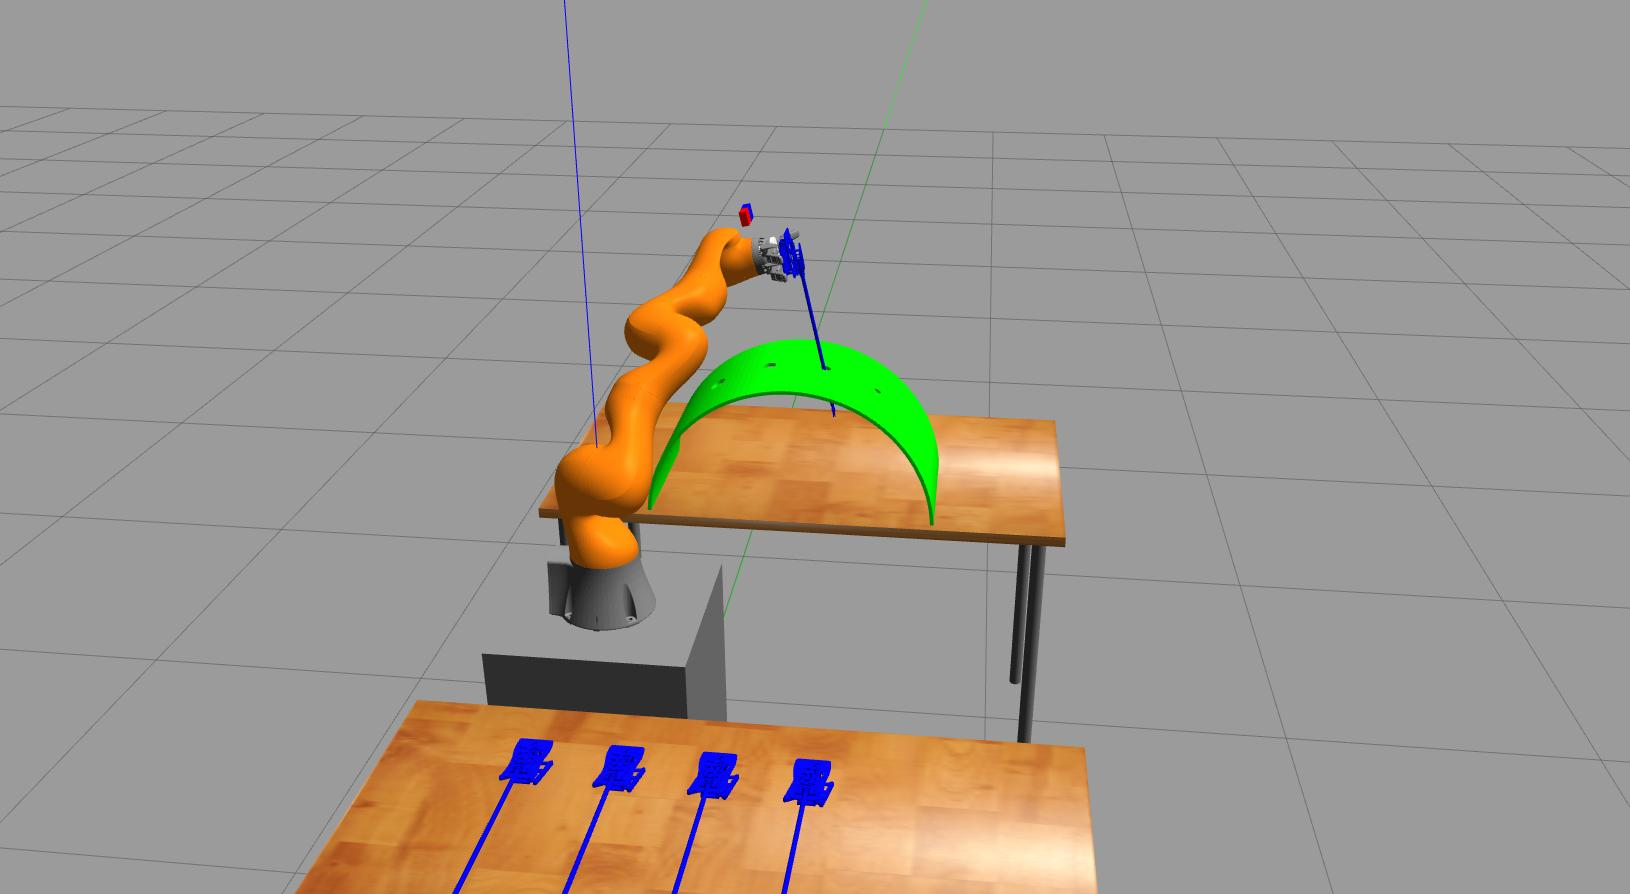
\includegraphics[width=0.3\textwidth]{images/robot_planner2/robot_planner2_8}\\
\caption{Experiment 2a:}
\label{experiment-robot-planner2a}
\end{figure}
\end{center}

To overcome the reachability issue shown in Figure \ref{experiment-robot-planner2a}, the algorithm was repeated, but this time using a different simulation layout 
in Gazebo, in which the mounting dock is closer to the robot and in front of it. This new layout enables the robot to reach all mounting holes with ease and 
with sufficient dexterity, the robot is free to pivot around.

\begin{center}
\begin{figure}[H]
\centering
\includegraphics[width=0.3\textwidth]{images/robot_planner2b/robot_planner2b_1}
\includegraphics[width=0.3\textwidth]{images/robot_planner2b/robot_planner2b_2}
\includegraphics[width=0.3\textwidth]{images/robot_planner2b/robot_planner2b_3}\\
\includegraphics[width=0.3\textwidth]{images/robot_planner2b/robot_planner2b_4}
\includegraphics[width=0.3\textwidth]{images/robot_planner2b/robot_planner2b_5}
\includegraphics[width=0.3\textwidth]{images/robot_planner2b/robot_planner2b_6}\\
\includegraphics[width=0.3\textwidth]{images/robot_planner2b/robot_planner2b_7}
\includegraphics[width=0.3\textwidth]{images/robot_planner2b/robot_planner2b_8}
\includegraphics[width=0.3\textwidth]{images/robot_planner2b/robot_planner2b_9}\\
\caption{Experiment 2b:}
\end{figure}
\end{center}

Due to the probabilistic nature of the motion planner (in these experiments the OMPL library is used with the RRTConnect path planning algorithm), the solutions 
to the path planning problem are not always the same and thus it is possible that the robot arm reaches a pose which is close to a singularity
\begin{center}
\begin{figure}[H]
\centering
\includegraphics[width=0.9\textwidth]{images/robot_planner2b/singularity_failure.png}
\caption{Experiment 2b: Singularity failure}
\end{figure}
\end{center}

\subsubsection{Robot Planner 3}

The goal of this third experiment is to design and test only some pivot trajectories. The pivot motions follow the equations described in 
\ref{subsection:pivot-motions}. The trajectories that were designed and tested in this experiments are the following:
\begin{itemize}
\item Circular
\item Arc
\item Line segment
\end{itemize}

\subsubsection{Robot Planner 4}

In this experiment we plan a simple pick-and-place path for a cube. The robotic arm first visits the left table and starts from the pre-grasp posture and then 
slowly approaches the cube until the grasp posture. When the gripper has reached the grasp posture, it closes the fingers to grasp the object and then retreats 
to the post-grasp posture. After that the robotic arm visits the right table to execute the place steps which are similar to the pick steps. The images below 
show some frames from the experiment with the first three to show the pick steps in the simulation environment and then other three images show the place steps 
in the visualization program.

\begin{center}
\begin{figure}[H]
\centering
\includegraphics[width=0.3\textwidth]{images/robot_planner4/robot_planner4_1}
\includegraphics[width=0.3\textwidth]{images/robot_planner4/robot_planner4_3}
\includegraphics[width=0.3\textwidth]{images/robot_planner4/robot_planner4_5}\\
\includegraphics[width=0.3\textwidth]{images/robot_planner4/robot_planner4_6}
\includegraphics[width=0.3\textwidth]{images/robot_planner4/robot_planner4_8}
\includegraphics[width=0.3\textwidth]{images/robot_planner4/robot_planner4_10}\\
\caption{Experiment 4: Simple pick-and-place experiment of a cube}
\end{figure}
\end{center}


\subsubsection{Robot Planner 5}

The goal of this fifth experiment is to control the KUKA robot using the camera via the visual servoing technique. In the first part of the experiment the 
robotic arm goes to an initial known position (e.g. the corner of the table) and then moves around until it detects a surgical tool. When that happens, the 
image-based visual servoing will send commands to the robot so that the detected tool is at the center of the video frame and with the same orientation 
as the video frame. At the second part of the experiment, the robot follows a similar algorithm. It starts with a known position, like the corner of the second 
table, then moves around until the mounting dock starts to appear inside the frame. When that happens, the image-based visual servoing will send commands to the 
robot so that the center of the trocar or the fulcrum reference frame is at the center and with the same orientation as the video frame. Similar results can be 
achieved by using position-based visual servoing, but that was not chosen at this implementation for simplicity and less operations. Position-based servoing 
requires more calculations because it is required to get the camera's transformation, express it with respect to the end-effector and then calculate the 
end-effector pose which is then used as an input to a Cartesian Controller.

\begin{center}
\begin{figure}[H]
\centering
\includegraphics[width=0.45\textwidth]{images/robot_planner5/visual_servo_controller3.png}
\includegraphics[width=0.45\textwidth]{images/robot_planner5/visual_servo_controller4.png}\\
\caption{Visual servo controller error diagrams. On the left image in the error graphs appear some spikes. These spikes occur from the sudden temporary detection 
of a nearby surgical tool. On the right image, these spikes are filtered out, and only the error graphs of the visual servoing of one tool are shown. The  
controller parameters are $K_p = 0.9, K_d = 0.2$}
\end{figure}
\end{center}

\begin{center}
\begin{figure}[H]
\centering
\includegraphics[width=0.6\textwidth]{images/grasp-points-triangle.png}\\
\caption{Image based visual servoing and calculation of grasp points. The yellow points are the grasp points and the thin black circumscribed circle is the growing circle that was used to calculate them.}
\end{figure}
\end{center}

\subsection{Results}

% Robot Planner 4 with RRTConnect
\begin{table}[H]
\centering
\scalebox{0.8}{
\begin{tabular}{|p{2cm}|c|p{2cm}|p{2cm}|p{2cm}|c|p{2cm}|p{2cm}|p{2cm}|}
\hline
                          & \multicolumn{8}{c}{\textbf{RRTConnect}}                                                                                                 \vline \\
\hline
Robot Planner 4           & \multicolumn{4}{c}{\textbf{Pick Pipeline}}                     \vline & \multicolumn{4}{c}{\textbf{Place Pipeline}}                     \vline \\
\hline
Experiment                & Status & Solution Time & Path Simplification Time & Planning Attempts & Status & Solution Time & Path Simplification Time & Planning Attempts  \\
\hline
1                         & 1      & 0.026189      & 0.065173                 & 1                 & 1      & 0.014644      & 0.020947                 & 1                  \\
2                         &        &               &                          &                   &        &               &                          &                    \\
3                         &        &               &                          &                   &        &               &                          &                    \\
4                         &        &               &                          &                   &        &               &                          &                    \\
5                         &        &               &                          &                   &        &               &                          &                    \\
\hline
\textbf{Average}          &        &               &                          &                   &        &               &                          &                    \\
\hline
\end{tabular}
}
\end{table}

% Robot Planner 4 with RRT*
\begin{table}[H]
\centering
\scalebox{0.8}{
\begin{tabular}{|p{2cm}|c|p{2cm}|p{2cm}|p{2cm}|c|p{2cm}|p{2cm}|p{2cm}|}
\hline
                          & \multicolumn{8}{c}{\textbf{RRT*}}                                                                                                 \vline \\
\hline
Robot Planner 4           & \multicolumn{4}{c}{\textbf{Pick Pipeline}}                     \vline & \multicolumn{4}{c}{\textbf{Place Pipeline}}                     \vline \\
\hline
Experiment                & Status & Solution Time & Path Simplification Time & Planning Attempts & Status & Solution Time & Path Simplification Time & Planning Attempts  \\
\hline
1                         &        &               &                          &                   &        &               &                          &                    \\
2                         &        &               &                          &                   &        &               &                          &                    \\
3                         &        &               &                          &                   &        &               &                          &                    \\
4                         &        &               &                          &                   &        &               &                          &                    \\
5                         &        &               &                          &                   &        &               &                          &                    \\
\hline
\textbf{Average}          &        &               &                          &                   &        &               &                          &                    \\
\hline
\end{tabular}
}
\end{table}

% Robot Planner 4 with PRM*
\begin{table}[H]
\centering
\scalebox{0.8}{
\begin{tabular}{|p{2cm}|c|p{2cm}|p{2cm}|p{2cm}|c|p{2cm}|p{2cm}|p{2cm}|}
\hline
                          & \multicolumn{8}{c}{\textbf{PRM*}}                                                                                                 \vline \\
\hline
Robot Planner 4           & \multicolumn{4}{c}{\textbf{Pick Pipeline}}                     \vline & \multicolumn{4}{c}{\textbf{Place Pipeline}}                     \vline \\
\hline
Experiment                & Status & Solution Time & Path Simplification Time & Planning Attempts & Status & Solution Time & Path Simplification Time & Planning Attempts  \\
\hline
1                         &        &               &                          &                   &        &               &                          &                    \\
2                         &        &               &                          &                   &        &               &                          &                    \\
3                         &        &               &                          &                   &        &               &                          &                    \\
4                         &        &               &                          &                   &        &               &                          &                    \\
5                         &        &               &                          &                   &        &               &                          &                    \\
\hline
\textbf{Average}          &        &               &                          &                   &        &               &                          &                    \\
\hline
\end{tabular}
}
\end{table}


%----------------------------------------------------------------------------------------
%	BIBLIOGRAPHY, REFERENCES, TABLES, APPENDIXES
%----------------------------------------------------------------------------------------
\newpage
\appendix
\appendixpage
\section{Software and Documentation}

\begin{itemize}
\item All software that developed for this thesis is available and will be maintained at \textbf{\url{https://github.com/karadalex/surgery_robotics_kuka_barrett}}
\item Instruction on how to run the software of this thesis, as well as documentation of the various software components is available and will be maintained at 
	\textbf{\url{https://karadalex.github.io/surgery_robotics_kuka_barrett/}}
\end{itemize}

\begin{center}
\begin{figure}[!htb]
\centering
\includegraphics[width=\textwidth]{images/documentation.png}
\caption{Documentation written with Sphinx and rosdoc\_lite }
\label{documentation}
\end{figure}
\end{center}

\section{Mathematics}

\subsection{Euler angles to Quaternions}

Let $\theta, \phi, \psi$ be the Euler angles (roll, pitch, yaw) respectively, then using the following equations
\[
cθ = \cos\left( \frac{θ}{2} \right) , sθ = \sin\left( \frac{θ}{2} \right)
\]
\[
cφ = \cos\left( \frac{φ}{2} \right) , sφ = \sin\left( \frac{φ}{2} \right)
\]
\[
cψ = \cos\left( \frac{ψ}{2} \right) , sψ = \sin\left( \frac{ψ}{2} \right)
\]

we can calculate the associated quaternion, in vector notation, as follows

\[
\mathbf{q} = \begin{bmatrix} q_x \\ q_y \\ q_z \\ q_w \end{bmatrix} = \begin{bmatrix}
sθcφcψ - cθsφsψ \\
cθsφcψ + sθcφsψ \\
cθcφsψ - sθsφcψ \\
cθcφcψ + sθsφsψ \\
\end{bmatrix}
\]

\subsection{Cartesian to spherical coordinates}

\[
r = \sqrt{x^2+y^2+z^2}
\]

\[
θ = atan2(\sqrt{x^2 + y^2}, z)
\]

\[
φ = atan2(y, x)
\]


\subsection{Spherical to cartesian coordinates}

\[
x = r\sin(θ)\cos(φ)
\]

\[
y = r\sin(θ)\sin(φ)
\]

\[
z = r\cos(θ)
\]



\newpage
\nomenclature{$^{i-1}T_{i}$}{Transformation matrix from coordinate frame $\lbrace i \rbrace$ to coordinate frame $\lbrace i-1 \rbrace$ }
\nomenclature{$c_{i}$}{Shorthand notation for $cosθ_{i}$}
\nomenclature{$s_{i}$}{Shorthand notation for $sinθ_{i}$}
\nomenclature{$^{i-1}R_{i}$}{Rotation matrix from coordinate frame $\lbrace i \rbrace$ to coordinate frame $\lbrace i-1 \rbrace$ }
\nomenclature{$^{i-1}\mathbf{p}_{iO}$}{Position vector from the origin of the coordinate frame $\lbrace i \rbrace$ to the origin of the coordinate frame $\lbrace i-1 \rbrace$ }
\nomenclature{$J^{\dagger}$}{Pseudoinverse of the Jacobian}
\nomenclature{$\mathcal{M}$}{Manipulability measure of the robotic arm}
\nomenclature{$\mathcal{L}_q$}{Dexterity measure of the robotic arm}
\nomenclature{$\hat{\mathbf{x}},\hat{\mathbf{y}},\hat{\mathbf{z}}$}{Unit vectors of $x,y,z$ axes respectively }
\nomenclature{$\hat{\mathbf{r}},\hat{\bm{\theta}},\hat{\bm{\phi}}$}{Unit vectors of $r,θ,φ$ axes respectively, in spherical coordinates }
\nomenclature{$\theta, \phi, \psi$}{roll, pitch, yaw angles, also known as the Euler angles}
\nomenclature{$\mathcal{C}$}{Configuration Space}
\nomenclature{$\mathcal{C}_{obs}$}{Obstacle Space}
\nomenclature{$\mathcal{C}_{free}$}{Free Configuration Space}
\nomenclature{$q_i$}{Angle position of joint $i$}
\nomenclature{$\dot{q}_i$}{Angle velocity of joint $i$}
\nomenclature{$\mathbf{q}$}{Angle positions vector of all joints}
\nomenclature{$\ddot{q}_i$}{Angle acceleration of joint $i$}
\nomenclature{$\dddot{q}_i$}{Angle jerk of joint $i$}
\nomenclature{$τ$}{Time constant, represents a specific time duration in a trajectory velocity profile or in a system controller}
\nomenclature{RCM}{Remote Center of Motion}
\nomenclature{TCP}{Tool's Center Point}
\nomenclature{$\mathbf{C}$}{Covariance matrix}
\nomenclature{$\mathbb{R}^n$}{Vector space of n-dimensional real-valued vectors}
\nomenclature{$\mathbb{R}^{n \times m}$}{Vector space of all real-valued $n \times m$ matrices}
\nomenclature{$SE(3)$}{Special Euclidean Group. Vector space of all 3D transformations}
\nomenclature{$SO(3)$}{Special Orthogonal Group. Vector space of all 3D rotations}
\nomenclature{$\mathbb{H}$}{Quaternions group. A four-dimenional space with basis $\mathbf{1},\mathbf{i},\mathbf{j},\mathbf{k}$ that includes all quaternions. In the context of this thesis quaternions are used for 3D rotations instead of matrices from $SO(3)$}
\nomenclature{$\mathbb{S}$}{Surgical 3D taskspace}
\nomenclature{$\mathbb{P}$}{Pivot paths 3D taskspace, $\mathbb{P} \subset \mathbb{T}$}
\nomenclature{$\mathbb{T}$}{Robot's Euclidean 3D taskspace}
\nomenclature{$\mathbb{J}$}{Joint taskspace}
\printnomenclature

\newpage
\cleardoublepage
\phantomsection
\listoffigures
\addcontentsline{toc}{section}{\listoflistingscaption}
\listoflistings
\listofalgorithms

\newpage
\nocite{*}
\printbibliography[heading=bibintoc,title={Bibliography}]

%\end{otherlanguage}
\end{document}
